\documentclass[11pt,a4paper]{report}


\title{The Network\\ 1. Milestone}
\author{Frank Steiler\\ DHBW Stuttgart / Staffordshire University\\ Student Number: 13005490d \\ Contact: frank@steiler.eu}
        
        
\usepackage[english]{babel}
\usepackage[english=british]{csquotes}
\usepackage[style=alphabetic,backend=biber,natbib=true]{biblatex}
\usepackage{graphicx}
\usepackage{setspace}
\usepackage{hyperref}
\usepackage{varioref}
\usepackage{chngcntr}
\usepackage{subcaption}
\usepackage[export]{adjustbox}[2011/08/13]
\usepackage{fancyhdr}
\usepackage[toc,page]{appendix}
\usepackage{pdfpages}
\usepackage{tabularx}
\usepackage{longtable}
\usepackage{float}
\usepackage{listings}
\usepackage{pifont}

\lstset{
    extendedchars=true,
    literate={->}{{\ding{213}}}1,
    moredelim=[is][\underbar]{_}{_}
}

\restylefloat{table}

\addbibresource{Milestone_1.bib}

\onehalfspacing


\pagestyle{fancy}
\lhead{}
\renewcommand{\headrulewidth}{0pt}
\setlength{\headheight}{14pt}

\newcommand{\nocontentsline}[3]{}
\newcommand{\tocless}[2]{\bgroup\let\addcontentsline=\nocontentsline#1{#2}\egroup}

\begin{document}

\counterwithout{figure}{chapter}
\counterwithout{table}{chapter}
\counterwithout{lstlisting}{chapter}

\newcounter{magicrownumbers}[table]
\newcommand\rownumber{\stepcounter{magicrownumbers}\arabic{magicrownumbers}}

\maketitle

\newpage
\thispagestyle{empty}
\mbox{}
\setcounter{page}{0}

\tableofcontents

\chapter{Introduction}
With the rise of the Internet and its increased accessibility more and more people started using this engineering marvel. With its help the whole mankind can stay connected, even if there are hundreds of miles away from each other. Over years and decades the way to handle this virtual wonderworld did change rapidly: Was it first the interaction via electronic mail staying connected got a complete new dimension when the first generation of so called "social networks" started to launch. \emph{Myspace} and \emph{Facebook} showed how popular and important it is with people to stay in contact. On top of that \emph{Twitter} created a quick way to share news and information. Social media and \emph{Twitter} especially played an important role within several important political events in the 21\textsuperscript{st} century. For example the networks were used to organize events during the Arab Spring \cite{ICT4DBibliography2170}.

2012 \emph{Facebook} went public and had the largest valuation for a new public company with \$104 billion\cite{FinTimes12}. Followed in 2013 by \emph{Twitter}, now even listed on the \emph{NYSE}. After its first day as a public company \emph{Twitter} was valued a little over \$31 billion \cite{BBCNews13}.

All these facts show the high acceptance of social media and their massive potential on the money market. Although it seems hard to built a new network from the scratch and to impose it. I believe there is many resentment against established networks that it is worth to do research and planning of a new web based social network. Following this document will try to initiate discussion and justify the the necessessity to introduce \emph{The Network}.

\chapter{Market Analysis}

The statistics about spreading of social networks are impressive. A survey by the Pew Research Center showed that 67\% of US citizens are using social network. Users are nearly equally distributed over all ages, genders and races \cite{PewResearch}. Facebook itself had 1.06 billion monthly user and 618 million daily user all over the world as of December 2012 \cite{FBReport}. From figure \vref{fig:MAU} it can be retrieved that the amount was constantly increasing over the year 2012. 
\begin{figure}[h]
    \centering
      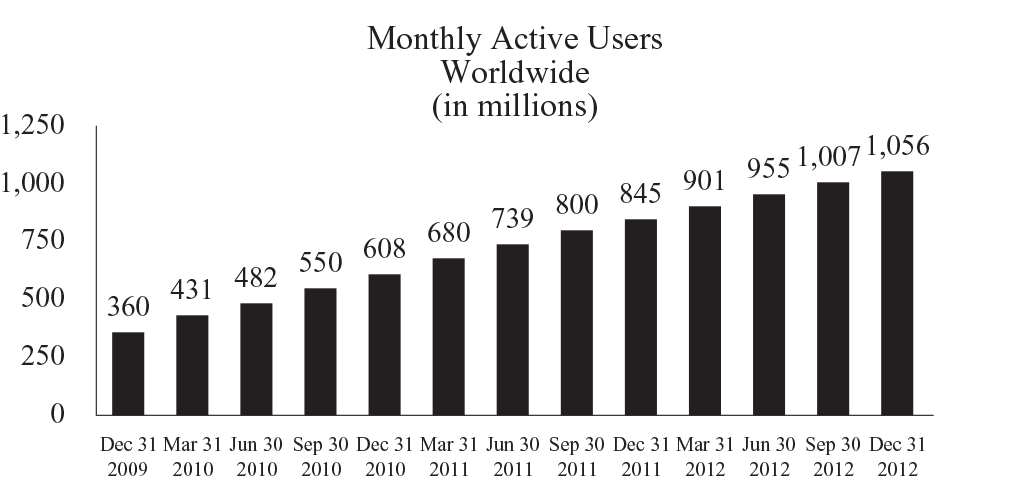
\includegraphics{./Pictures/MAU_FB.png}
      \caption[Monthly active users of \emph{Facebook} retrieved from \cite{FBReport}]{Monthly active users of \emph{Facebook}}
      \label{fig:MAU}
\end{figure}
It appears that the market does not have any potential for a really big growth in the near future, since nearly every possible user already has got a well connected social media account. So where should be any need in developing a new social network? The reasons are going to be discussed in the following sections.

\section{Lifecycle of social media}
In 2007 \emph{Myspace} was the most popular social network, and nobody thought that within a few years the former \emph{king} could loose its crown. From figure \vref{fig:myspace} it can be retrieved that the interest in this network reached its climax by 2008. But then \emph{Facebook} took over the lead and started to outclass \emph{Myspace}. As \textcite{Dube:2013aa} stated it is possible that \emph{Facebook} --currently \enquote{king of the hill}-- could possible loose it's head start within the next couple of years to another competitor, just like it happened years before.
\begin{figure}[h]
\centering
\begin{subfigure}{.5\textwidth}
  \centering
  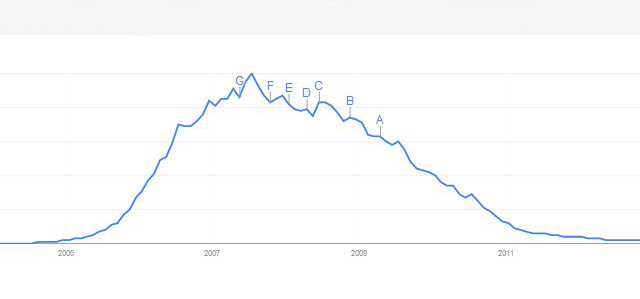
\includegraphics[width=0.98\linewidth]{./Pictures/facebook-myspace1.jpg}
  \caption{\emph{Myspace} (blue) 2004-2011}
  \label{fig:myspace}
\end{subfigure}%
\begin{subfigure}{.5\textwidth}
  \centering
  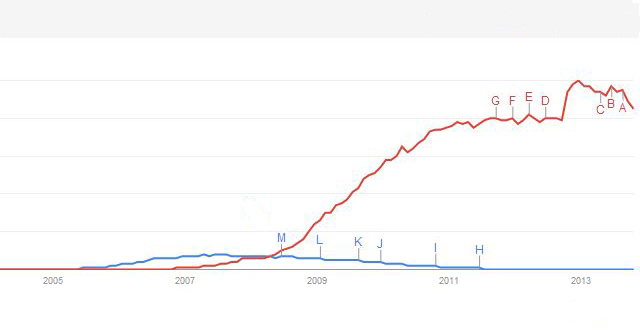
\includegraphics[width=0.98\linewidth]{./Pictures/facebook-myspace2.jpg}
  \caption{\emph{Myspace} (blue) \& \emph{Facebook} (red) 2005-2014}
  \label{fig:myspace+fb}
\end{subfigure}
\caption[Interest on Social Networks over time 
 \emph{Google Trends} retrieved from \cite{Dube:2013aa}]{Interest on Social Networks over time according to \emph{Google Trends}}
\label{fig:google_trends}
\end{figure}
This theory is supported by a recent study by researchers from Princeton. Their paper uses a statistical model which also fitted to the decline of \emph{Myspace}. It states that \emph{Facebook} will loose 80\% of their users between 2015 and 2017 \cite{Cannarella:2014aa}. 
\begin{figure}[h]
    \centering
      \includegraphics[width=1.1\textwidth,center]{./Pictures/facebook-myspace-prediction}
      \caption[Princeton model applied to \emph{Mypace} and \emph{Facebook} retrieved from \cite{Cannarella:2014aa}]{Princeton model applied to \emph{Mypace} and \emph{Facebook}}
      \label{fig:Princeton}
\end{figure}
As shown in figure \vref{fig:Princeton} the so called \emph{irSIR} and \emph{SIR} model matches very good to the history of \emph{Myspace}. If we adopt the curve to \emph{Facebook}'s current development there is an early and late border for the predicted end of the network. Of course such a significant progress doesn't happen without any reason. Such reasons are currently heavily discussed by critics among the undisputed criticism to a lax handling of user data. The next chapters will focus on these points.

\section{Aging of the user basis}
\emph{Facebook}'s amount of users is constantly increasing since its release many years ago. But not only the amount of active users is important for the continued existence of a popular social network. It is also important to be attractive for younger user. That is currently a very big problem of the long-established social networks. A recent report of \emph{iStrategyLabs} based on \emph{Facebook}'s \emph{Social Advertising} platform showed that the number of users between the age of 13 and 17 decreased by 25\% since 2011. Also the age group of 18 up to 24 years old lost nearly 8\% of their users \cite{Saul:2014aa} . The biggest growth of users on \emph{Facebook} has been in the group of people who are older than 55 years. On top of that there are 6.7 million fewer people in these demographics. These people got rid of their accounts and signed out of the social network. As \textcite{Neal:2014aa} says, \enquote{there is nothing cool about having parents and grandparents “liking” pictures of your friends.}. Furthermore he says that the younger generations are using newer messaging services like \emph{Instagram}, \emph{Snapchat} or \emph{WhatsApp} more likely than a big social network, because of an easy usage and an increased privacy of messages in opposite to the public postings at \emph{Facebook} \cite{Neal:2013aa}.

\section{Overwhelming Advertisement}
Of course it is very expensive to run a platform like \emph{Facebook}. Since the business model of \emph{Facebook} is  based on a free usage for the end-user it was important to make money by selling personalized advertisement. Besides showing traditional banner alongside or on top of the page \emph{Facebook} introduced \emph{sponsored posts}. These are posts of paying customer, mainly companies, which are shown at the front page like every status of the friends of a user. But they appear even if the user doesn't \emph{like} the advertising page. Many user are enraged and complain about to only see ads \cite{Sloane:2013aa}. This is resulting in loosing users because of dissatisfaction. The \emph{MIT Technology Review} states another problem connected with adverts. It shows that the overall revenue of advertisement per user is constantly decreasing. \emph{Facebook} is only able to compensate this by increasing user count. Since this model is currently declining \emph{Facebook} will struggle with lower revenues but constant maintenance costs \cite{Wolff:2012aa}. Concluding \emph{Facebook} is not only loosing users but also revenues, a combination that can kill every business.

\section{Conclusion}
Summing up all of the facts leads to one conclusion: The market situation is going to change and \emph{Facebook} will probably loose its lead. But that only will happen if there is going to be a better alternative. All the negative items mentioned above have to be improved to a new network giving a real alternative to current services. By considering all these aspects this project can get an enhanced and widely accepted new social platform that will grow for years and produce big revenue for its owner.

\chapter{Software Requirement Specification}
Within the next sections the functional requirements of \emph{The Network}, a web based social network, will be outlined. The project is going to be developed as part of the \emph{Web Programming with Servlets and Java Server Pages} lecture held at the Staffordshire University 2014.

\section{Product Purpose}

The development of \emph{The Network} should take account of the known problems of competitors. The outcome of this project should be a durable, easy-to-use and well designed social network. On top of that it should be competitive with existing services and based on the platform independent technologies \emph{Java Server Pages}, \emph{Java Servlets} and \emph{Java}.

\subsection{Definitions}
To better understand the following sections it is important to define several terms. These definitions are shown in table \vref{tab:definition}.

\begin{table}
    \begin{tabularx}{\textwidth}{l | X}
        Term & Description \\ \hline
        \emph{Normal user} & The representation of a person on the social network \\
        \\
        \emph{Fanpage} & The representation of an interest group, a club or a company. This page can be administrated by a single person or a whole department. \\
    \end{tabularx}
\caption{Definition of specific terms}
\label{tab:definition}
\end{table}


\subsection{Obligatory Requirements}
The fulfillment of the following criteria is mandatory:
\begin{itemize}
    \item Every user can create an own profile.
    \item Every user can create an own fanpage.
    \item Every fanpage can be connected to one user.
    \item There are admin accounts which can delete user and fanpages.
    \item Ever admin account can be connected to one user.
    \item Only the user can delete the connection to a fanpage or admin account.
    \item A user can follow a fanpage.
    \item A user can ask another user to be a friend. This \emph{friendship} is only established after the other user accepts the friend request.
    \item Every user can delete the friendship with a user or un-follow a fanpage.
    \item Every user can publish a status post. He has the choice to post it public (for everyone) or private (only for friends).
    \item Every fanpage can only publish public status posts.
    \item The user can read all posts of friends and followed pages.
    \item The user can read all public posts of all users and pages.
    \item The user can comment on every post he is allowed to read.
    \item A fanpage can only comment on posts published by itself.
    \item The user can up-/down-vote every comment and status he is allowed to read.
    \item The user can only send messages to friends.
    \item The user gets notified if there are new messages, comments on posts he is following or a new friend request.
    \item Every user can change/delete its profile.
    \item Every fanpage can change/delete its page.
    \item The software needs to be programmed using GNU General Public License 3 (GPLv3).
\end{itemize}

\subsection{Optional Requirements}
An optional functionality is the development of an application programming interface (API), which provides a secure connection between applications and  the  server  without the web interface. Within the project it is optional to prove the functionality of this interface by developing a java-based desktop application. This application should use XML-based communication and needs to have a professional standard graphical user interface (GUI).

\subsection{Non-Requirements}
The fulfillment of the following criteria is \textbf{not} part of the project:
\begin{itemize}
    \item A fanpage cannot access any profile or fanpage.
    \item A fanpage cannot send or receive messages.
    \item A fanpage cannot see any status of users and therefor it won't be able to comment, down- or up-vote it.
    \item The admin account will not be able to post, comment, read, vote or manipulate any post or comment of any user.
    \item The admin account cannot read any messages.
    \item The admin account cannot send or receive any messages.
    \item An admin account cannot be created within the web or application interface.
    \item No one can upload photos besides the profile photo.
    \item Signing up or paying for a premium account is not considered within this version.
\end{itemize}

\section{User}
The key to develop a good application is the user. If the application is not focused on the user group it won't get accepted. The designated user group is going to be defined in the following section.
\subsection{User characteristics}
An open social network is only useful for an user if his friends, people he is interested in or organizations he wants to keep track of are part of the network. That's why the project does not have a specific user group, but needs to cover all possible users. If we focus on technical acceptance there is still a big diversity within the society based on the age. That's why our focus target group for a new launched social network is going to be the younger generations (Under 30). But we have to keep in mind that while the project is growing the user group will definitely expand to all age groups. So the design of the product needs to be as simple and intuitive as possible. To keep it simple the user interface (UI) needs to be clean. On top of that the range of functions is going to be reduced to the minimum so nobody is going to be put off because of an overwhelming amount of options. 
\subsection{User types}
All analysis lead to 6 user types specified in table \vref{tab:usertypes}.

\begin{table}
    \begin{tabularx}{\textwidth}{l | X}
        Usertype & Description \\ \hline
        \emph{Guest user} & This is a user, which is not subscribed to the network. He will not have the possibility to explore the network unless he signs up for the service. \\
        \\
        \emph{Normal free user} & This user is a normal person exploring the social network. He does not pay for the use of the network, but there are going to be advertisements on every page. \\
        \\
        \emph{Normal premium user} & This user is a normal person exploring the social network. He pays for the use of the network, so there are not going to be any advertisements. \\
        \\
        \emph{Free fanpage admin} & This user administrates a fanpage, where he represents a society, company or interest group. He does not pay for the use of the network, but there are going to be advertisements on every page. \\
        \\
        \emph{Premium fanpage admin} & This user administrates a fanpage, where he represents a society, company or interest group. He pays for the use of the network, so there are not going to be any advertisements. \\
        \\
        \emph{Admin user} & This user administrates the network. He is able to view statistics and delete users or fanpages.\\
    \end{tabularx}
\caption{Specification of user types within \emph{The Network}}
\label{tab:usertypes}
\end{table}

\section{Use-cases}
Use-cases are an important step to define the project in a detailed way. The UML use case diagram which will give an overview for the project can be found in appendix \vref{app:Use-Case_Diagram_TheNetwork}. Every use case is going to be described according to \textcite{Cockburn:2001aa}.

\subsection{Manage friends \& followed pages use-case}
The Manage friends \& followed pages use-case describes how a user can manage his connections within the network. The user is able to add and remove friends and fanpages. The UML use case diagram for this use case can be found in appendix \vref{app:Use-Case_Diagram_ManageFriends}.

\subsubsection{Use case: Show all friends}

\begin{longtable}{p{.23\textwidth} | p{.72\textwidth}}
    \caption{Use case: Show all friends} \label{tab:ucShowFriends} \\
    \endfirsthead
        \multicolumn{2}{c}
        {{\bfseries \tablename\ \thetable{} -- continued from previous page}} \\
        \multicolumn{2}{c}{} \\
    \endhead
        \multicolumn{2}{c}{{Continued on next page}} \\ 
    \endfoot
    \endlastfoot
    
        \hline
        \emph{Description:} & A user wants an overview of all his friends.\\
        \emph{Actors:} & 
            \begin{itemize} 
                \item User
                \item Friend / Page Following Management Service
             \end{itemize} \\
        \emph{Pre-Conditions:} & 
            \begin{itemize} 
                \item User is logged in.
             \end{itemize} \\
        \emph{Post-Conditions:} & \textbf{Success guarantees:} 
            \begin{itemize} 
                \item The user sees a list of all his friends.
             \end{itemize} \\
        \emph{Normal flow:} & 
            \begin{enumerate} 
                \item User clicks on the "Friends" entry in the header bar.
                \item The systems collects all his friends.
                \item All friends are listed on the next page.
             \end{enumerate} \\
             \hline
\end{longtable}

\subsubsection{Use case: Show all followed pages}

\begin{longtable}{p{.23\textwidth} | p{.72\textwidth}}
    \caption{Use case: Show all followed pages} \label{tab:ucShowPages} \\
    \endfirsthead
        \multicolumn{2}{c}
        {{\bfseries \tablename\ \thetable{} -- continued from previous page}} \\
        \multicolumn{2}{c}{} \\
    \endhead
        \multicolumn{2}{c}{{Continued on next page}} \\ 
    \endfoot
    \endlastfoot
    
        \hline
        \emph{Description:} & A user wants an overview of all pages he is following.\\
        \emph{Actors:} & 
            \begin{itemize} 
                \item User
                \item Friend / Page Following Management Service
             \end{itemize} \\
        \emph{Pre-Conditions:} & 
            \begin{itemize} 
                \item User is logged in.
             \end{itemize} \\
        \emph{Post-Conditions:} & \textbf{Success guarantees:} 
            \begin{itemize} 
                \item The user sees a list of all pages he is following.
             \end{itemize} \\
        \emph{Normal flow:} & 
            \begin{enumerate} 
                \item User clicks on the "Fanpages" entry in the header bar.
                \item The systems collects all his followed pages.
                \item All followed pages are listed on the next page.
             \end{enumerate} \\
             \hline
\end{longtable}

\subsubsection{Use case: Follow a page}

\begin{longtable}{p{.23\textwidth} | p{.72\textwidth}}
    \caption{Use case: Follow a page} \label{tab:ucFollowPage} \\
    \endfirsthead
        \multicolumn{2}{c}
        {{\bfseries \tablename\ \thetable{} -- continued from previous page}} \\
        \multicolumn{2}{c}{} \\
    \endhead
        \multicolumn{2}{c}{{Continued on next page}} \\ 
    \endfoot
    \endlastfoot
    
        \hline
        \emph{Description:} & If a user is interested in a fanpage and wants to keep track of it he will follow this page.\\
        \emph{Actors:} & 
            \begin{itemize} 
                \item User
                \item Friend / Page Following Management Service
             \end{itemize} \\
        \emph{Pre-Conditions:} & 
            \begin{itemize} 
                \item User is not following the page.
                \item User has found and opened the homepage of the fanpage.
             \end{itemize} \\
        \emph{Post-Conditions:} & \textbf{Success guarantees:} 
            \begin{itemize} 
                \item System adds the fanpage to the list of followed pages of the user.
             \end{itemize} \\
        \emph{Normal flow:} & 
            \begin{enumerate} 
                \item User clicks on the "Follow page" button.
                \item The systems adds the fanpage to the social profile of the user.
                \item The system reloads the fanpage, indicating the following of the page by replacing the "Follow page" button with an "Unfollow page" button.
             \end{enumerate} \\
             \hline
\end{longtable}

\subsubsection{Use case: Add a friend}

\begin{longtable}{p{.23\textwidth} | p{.72\textwidth}}
    \caption{Use case: Add a friend} \label{tab:ucAddFriend} \\
    \endfirsthead
        \multicolumn{2}{c}
        {{\bfseries \tablename\ \thetable{} -- continued from previous page}} \\
        \multicolumn{2}{c}{} \\
    \endhead
        \multicolumn{2}{c}{{Continued on next page}} \\ 
    \endfoot
    \endlastfoot
    
        \hline
        \emph{Description:} & If a user (A) is interested in another person (B) and wants to stay in contact with the other user (B) he will ask for a virtual friendship.\\
        \emph{Actors:} & 
            \begin{itemize} 
                \item User (A)
                \item Friend / Page Following Management Service
             \end{itemize} \\
        \emph{Pre-Conditions:} & 
            \begin{itemize} 
                \item User (A) is no friend of the other user (B).
                \item User (A) has not added the other user (B) in the past as a friend.
                \item User (A) has found and opened the profile of the other user (B).
             \end{itemize} \\
        \emph{Post-Conditions:} & \textbf{Success guarantees:} 
            \begin{itemize} 
                \item System stores the friend request.
                \item The added user (B) receives a friend request.
             \end{itemize} \\
        \emph{Normal flow:} & 
            \begin{enumerate} 
                \item User (A) clicks on the "Add as friend" button on the profile page of the other user (B).
                \item The systems stores the request.
                \item The added user (B) receives a friend request.
                \item The system reloads the profile page, indicating the open friend request by replacing the "Add as friend" button with a "Request pending" button.
             \end{enumerate} \\
             \hline
\end{longtable}

\subsubsection{Use case: Accept a friend}

\begin{longtable}{p{.23\textwidth} | p{.72\textwidth}}
    \caption{Use case: Accept a friend} \label{tab:ucAcceptFriend} \\
    \endfirsthead
        \multicolumn{2}{c}
        {{\bfseries \tablename\ \thetable{} -- continued from previous page}} \\
        \multicolumn{2}{c}{} \\
    \endhead
        \multicolumn{2}{c}{{Continued on next page}} \\ 
    \endfoot
    \endlastfoot
    
        \hline
        \emph{Description:} & If a user (B) is interested in a virtual friendship with another user (A), the  other user (A) has to accept this request if he wants to be a friend.\\
        \emph{Actors:} & 
            \begin{itemize} 
                \item User (A)
                \item Friend / Page Following Management Service
             \end{itemize} \\
        \emph{Pre-Conditions:} & 
            \begin{itemize} 
                \item Other user (B) is no friend of the user.
                \item Other user (B) has sent a request to the user (A).
             \end{itemize} \\
        \emph{Post-Conditions:} & \textbf{Success guarantees:} 
            \begin{itemize} 
                \item Friendship added to social profile of both user.
                \item The other user (B) gets notified that he is now a friend of the user (A).
             \end{itemize} \\
        \emph{Normal flow:} & 
            \begin{enumerate} 
                \item User (A) clicks on the "Friends" menu item.
                \item User (A) clicks on the "Accept" button next to the profile of the other user (B).
                \item The systems stores the change of the friendship status.
                \item The systems sets a notification flag, to notify the other user (B).
                \item The system reloads the page, indicating the successful adding of the friend by removing the request and adding the user (B) to the "Friends" list.
             \end{enumerate} \\
             \hline
\end{longtable}
\pagebreak
\subsubsection{Use case: Reject a friend}

\begin{longtable}{p{.23\textwidth} | p{.72\textwidth}}
    \caption{Use case: Reject a friend} \label{tab:ucRejectFriend} \\
    \endfirsthead
        \multicolumn{2}{c}
        {{\bfseries \tablename\ \thetable{} -- continued from previous page}} \\
        \multicolumn{2}{c}{} \\
    \endhead
        \multicolumn{2}{c}{{Continued on next page}} \\ 
    \endfoot
    \endlastfoot
    
        \hline
        \emph{Description:} & If a user (B) is interested in a virtual friendship with another user (A), the other user (A) has to reject this request if he does not want to be a friend with the user (B).\\
        \emph{Actors:} & 
            \begin{itemize} 
                \item User (A)
                \item Friend / Page Following Management Service
             \end{itemize} \\
        \emph{Pre-Conditions:} & 
            \begin{itemize} 
                \item Other user (B) is no friend of the user (A).
                \item Other user (B) has sent a request to the user (A).
             \end{itemize} \\
        \emph{Post-Conditions:} & \textbf{Success guarantees:} 
            \begin{itemize} 
                \item Friend request gets rejected.
                \item The other user (B) is not able to resend a friend request to user (A).
             \end{itemize} \\
        \emph{Normal flow:} & 
            \begin{enumerate} 
                \item User (A) clicks on the "Friends" menu item.
                \item User (A) clicks on the "Reject" button next to the profile of the other user (B).
                \item The systems stores the change of the friendship status.
                \item The system reloads the page, indicating the successful rejection of the friend by removing the request.
             \end{enumerate} \\
             \hline
\end{longtable}

\subsubsection{Use case: Stop following a page}

\begin{longtable}{p{.23\textwidth} | p{.72\textwidth}}
    \caption{Use case: Stop following a page} \label{tab:ucUnFollowPage} \\
    \endfirsthead
        \multicolumn{2}{c}
        {{\bfseries \tablename\ \thetable{} -- continued from previous page}} \\
        \multicolumn{2}{c}{} \\
    \endhead
        \multicolumn{2}{c}{{Continued on next page}} \\ 
    \endfoot
    \endlastfoot
    
        \hline
        \emph{Description:} & If a user is no longer interested in a fanpage, he will stop following this page.\\
        \emph{Actors:} & 
            \begin{itemize} 
                \item User
                \item Friend / Page Following Management Service
             \end{itemize} \\
        \emph{Pre-Conditions:} & 
            \begin{itemize} 
                \item User follows the fanpage.
                \item User found the fanpage in the fanpage overview or found the fanpage itself.
             \end{itemize} \\
        \emph{Post-Conditions:} & \textbf{Success guarantees:} 
            \begin{itemize} 
                \item Fanpage gets removed from the social profile of the user.
             \end{itemize} \\
        \emph{Normal flow:} & 
            \begin{enumerate} 
                \item User clicks on the "Unfollow" button next to the page within the list or on the fanpage itself.
                \item The system deletes the fanpage from the social profile of the user.
                \item The system reloads the page indicating the success by removing the fanpage from the fan page overview list or replacing the "Unfollow" button with a "Follow page" button.
             \end{enumerate} \\
             \hline
\end{longtable}

\subsubsection{Use case: Remove a friend}

\begin{longtable}{p{.23\textwidth} | p{.72\textwidth}}
    \caption{Use case: Remove a friend} \label{tab:ucRemoveFriend} \\
    \endfirsthead
        \multicolumn{2}{c}
        {{\bfseries \tablename\ \thetable{} -- continued from previous page}} \\
        \multicolumn{2}{c}{} \\
    \endhead
        \multicolumn{2}{c}{{Continued on next page}} \\ 
    \endfoot
    \endlastfoot
    
        \hline
        \emph{Description:} & If a user (A) does not want to be a friend with another user (B) anymore, he will delete this user (B)\\
        \emph{Actors:} & 
            \begin{itemize} 
                \item User (A)
                \item Friend / Page Following Management Service
             \end{itemize} \\
        \emph{Pre-Conditions:} & 
            \begin{itemize} 
                \item User (A) is friend of the other user (B).
                \item User (A) found the user (B) in the friends overview or found the profile page of the user (B).
             \end{itemize} \\
        \emph{Post-Conditions:} & \textbf{Success guarantees:} 
            \begin{itemize} 
                \item Both users get removed from the social profile of each other.
             \end{itemize} \\
        \emph{Normal flow:} & 
            \begin{enumerate} 
                \item User clicks on the "Remove friend" button next to the profile within the list or on the profile page itself.
                \item The system deletes both users from each others profile.
                \item The system relaods the page indicating the success by removing the user (B) from the friends overview list of user (A) or replacing the "Remove friend" button with a "Add friend" button.
             \end{enumerate} \\
             \hline
\end{longtable}

\subsection{Access control use-case}
The Login use-case describes how existing and new users can access the social network. The UML use case diagram for this use case can be found in appendix \vref{app:Use-Case_Diagram_Access_Control}.

\subsubsection{Use case: Log-in}

\begin{longtable}{p{.23\textwidth} | p{.72\textwidth}}
    \caption{Use case: Sign-in} \label{tab:ucLogIn} \\
    \endfirsthead
        \multicolumn{2}{c}
        {{\bfseries \tablename\ \thetable{} -- continued from previous page}} \\
        \multicolumn{2}{c}{} \\
    \endhead
        \multicolumn{2}{c}{{Continued on next page}} \\ 
    \endfoot
    \endlastfoot
    
        \hline
        \emph{Description:} & If a user wants to use the network he needs to sign into the network.\\
        \emph{Actors:} & 
            \begin{itemize} 
                \item User
                \item Page admin
                \item Admin
                \item User Management Service
             \end{itemize} \\
        \emph{Pre-Conditions:} & 
            \begin{itemize} 
                \item User is already signed up for the social network.
                \item User is currently not signed in.
             \end{itemize} \\
        \emph{Post-Conditions:} & \textbf{Success guarantees:} 
            \begin{itemize} 
                \item System logs the user into his account.
             \end{itemize} \\
        \emph{Normal flow:} & 
            \begin{enumerate} 
                \item User enters his credential and clicks the "Log in" button.
                \item The systems validates the credentials.
                \item The system forwards the user to his homepage depending on the type of user (Normal user homepage, Fanpage admin homepage or Admin homepage).
             \end{enumerate} \\
        \emph{Alternative flow:} & If the provided credentials are not valid the system is going to redirect the user back to the log in page where he will be able to re-enter the right credentials.\\ 
             \hline
\end{longtable}
\pagebreak
\subsubsection{Use case: Sign-up as normal user}

\begin{longtable}{p{.23\textwidth} | p{.72\textwidth}}
    \caption{Use case: Sign-up as normal user} \label{tab:ucSignUpNormal} \\
    \endfirsthead
        \multicolumn{2}{c}
        {{\bfseries \tablename\ \thetable{} -- continued from previous page}} \\
        \multicolumn{2}{c}{} \\
    \endhead
        \multicolumn{2}{c}{{Continued on next page}} \\ 
    \endfoot
    \endlastfoot
    
        \hline
        \emph{Description:} & If a guest user wants to join and use the social network he needs to sign up.\\
        \emph{Actors:} & 
            \begin{itemize} 
                \item Guest
                \item User Management Service
             \end{itemize} \\
        \emph{Pre-Conditions:} & 
            \begin{itemize} 
                \item The guest is not signed up for the social network.
             \end{itemize} \\
        \emph{Post-Conditions:} & \textbf{Success guarantees:} 
            \begin{itemize} 
                \item The system creates a new user and logs him into his account.
             \end{itemize} \\
        \emph{Normal flow:} & 
            \begin{enumerate} 
                \item User enters the requested details about himself and clicks on the "Sign up as a normal user" button
                \item The systems creates a new account.
                \item The systems invokes the log in function to log the user into his account
                \item The system forwards the user to his homepage for a normal user.
             \end{enumerate} \\
        \emph{Alternative flow:} & If the user enters invalid information or not enough information the system will redirect him to the log in page to fill or correct the missing or wrong information.\\ 
             \hline
\end{longtable}
\pagebreak
\subsubsection{Use case: Sign-up as fanpage admin}

\begin{longtable}{p{.23\textwidth} | p{.72\textwidth}}
    \caption{Use case: Sign-up as fanpage admin} \label{tab:ucSignUpFanpage} \\
    \endfirsthead
        \multicolumn{2}{c}
        {{\bfseries \tablename\ \thetable{} -- continued from previous page}} \\
        \multicolumn{2}{c}{} \\
    \endhead
        \multicolumn{2}{c}{{Continued on next page}} \\ 
    \endfoot
    \endlastfoot
    
        \hline
        \emph{Description:} & If a interest group or company wants to join and use the social network they need to sign up.\\
        \emph{Actors:} & 
            \begin{itemize} 
                \item Guest
                \item User Management Service
             \end{itemize} \\
        \emph{Pre-Conditions:} & 
            \begin{itemize} 
                \item The guest is not signed up for the social network.
             \end{itemize} \\
        \emph{Post-Conditions:} & \textbf{Success guarantees:} 
            \begin{itemize} 
                \item The system creates a new fanpage and logs the user into his account.
             \end{itemize} \\
        \emph{Normal flow:} & 
            \begin{enumerate} 
                \item User enters the requested details about the group or company and clicks on the "Sign up as a fanpage admin" button
                \item The systems creates a new account.
                \item The systems invokes the log in function to log the user into his account
                \item The system forwards the user to his homepage for an fanpage admin user.
             \end{enumerate} \\
        \emph{Alternative flow:} & If the user enters invalid information or not enough information the system will redirect him to the log in page to fill or correct the missing or wrong information.\\ 
             \hline
\end{longtable}
\pagebreak
\subsubsection{Use case: Log-out}

\begin{longtable}{p{.23\textwidth} | p{.72\textwidth}}
    \caption{Use case: Log-out} \label{tab:ucLogout} \\
    \endfirsthead
        \multicolumn{2}{c}
        {{\bfseries \tablename\ \thetable{} -- continued from previous page}} \\
        \multicolumn{2}{c}{} \\
    \endhead
        \multicolumn{2}{c}{{Continued on next page}} \\ 
    \endfoot
    \endlastfoot
    
        \hline
        \emph{Description:} & If the user leaves the computer he needs to log himself out.\\
        \emph{Actors:} & 
            \begin{itemize} 
                \item User
                \item Page admin
                \item Admin
                \item User Management Service
             \end{itemize} \\
        \emph{Pre-Conditions:} & 
            \begin{itemize} 
                \item User is logged-in.
             \end{itemize} \\
        \emph{Post-Conditions:} & \textbf{Success guarantees:} 
            \begin{itemize} 
                \item The user is logged out of the system and needs to reenter his credential before using the service again.
             \end{itemize} \\
        \emph{Normal flow:} & 
            \begin{enumerate} 
                \item The user selects the "Log-out" item from the drop down menu on the top of the page.
                \item The system refreshes the page.
                \item The system presents the Log-in page, showing that the user was successfully logged out.
             \end{enumerate} \\
             \hline
\end{longtable}
\pagebreak
\subsubsection{Use case: Switch to connected user}

\begin{longtable}{p{.23\textwidth} | p{.72\textwidth}}
    \caption{Use case: Switch to connected user} \label{tab:ucSwitchCon} \\
    \endfirsthead
        \multicolumn{2}{c}
        {{\bfseries \tablename\ \thetable{} -- continued from previous page}} \\
        \multicolumn{2}{c}{} \\
    \endhead
        \multicolumn{2}{c}{{Continued on next page}} \\ 
    \endfoot
    \endlastfoot
    
        \hline
        \emph{Description:} & If there are fan page administrator profiles or system administrator profiles connected to a user it is possible to quick switch between them.\\
        \emph{Actors:} & 
            \begin{itemize} 
                \item User
                \item Page admin
                \item Admin
                \item User Management Service
             \end{itemize} \\
        \emph{Pre-Conditions:} & 
            \begin{itemize} 
                \item Normal User, Fanpage admin or System administrator is logged-in.
                \item There are other profiles connected to the current user
             \end{itemize} \\
        \emph{Post-Conditions:} & \textbf{Success guarantees:} 
            \begin{itemize} 
                \item The user is able to use the service, as if he would have logged himself in as the connected user.
             \end{itemize} \\
        \emph{Normal flow:} & 
            \begin{enumerate} 
                \item The user selects the name of the connected profile from the drop down menu on the top of the page.
                \item The system refreshes the page.
                \item The system presents the homepage of the selected profile.
             \end{enumerate} \\
             \hline
\end{longtable}

\subsection{Postings use-case}
The Posting use-case describes how a user or fanpage can share information with other users by posting and commenting. The UML use case diagram for this use case can be found in appendix \vref{app:Use-Case_Diagram_Postings}.

\subsubsection{Use case: Publish posts}

\begin{longtable}{p{.23\textwidth} | p{.72\textwidth}}
    \caption{Use case: Publish posts} \label{tab:ucPubPosts} \\
    \endfirsthead
        \multicolumn{2}{c}
        {{\bfseries \tablename\ \thetable{} -- continued from previous page}} \\
        \multicolumn{2}{c}{} \\
    \endhead
        \multicolumn{2}{c}{{Continued on next page}} \\ 
    \endfoot
    \endlastfoot
    
        \hline
        \emph{Description:} & If a user of fanpage want to share information with their friends or the whole network they can publish a post.\\
        \emph{Actors:} & 
            \begin{itemize} 
                \item User
                \item Page Admin
                \item Posting and Comment Service
             \end{itemize} \\
        \emph{Pre-Conditions:} & 
            \begin{itemize} 
                \item The user is logged into the system.
                \item The user is viewing his homepage.
             \end{itemize} \\
        \emph{Post-Conditions:} & \textbf{Success guarantees:} 
            \begin{itemize} 
                \item The system stores the status post and presents it to the people who are allowed to view the post.
             \end{itemize} \\
        \emph{Normal flow:} & 
            \begin{enumerate} 
                \item The user enters the status he wants to publish in the "Update your status here" textfield.
                \item The user presses the "Post" button to publish the post.
                \item The system checks the input and stores the post.
                \item The post appears in the profile of the user. 
             \end{enumerate} \\
        \emph{Alternative flow:} & If the user is a normal (premium) user he is able to mark a post as \emph{private}, so it can only be viewed by friends. If the status was empty the system will give an error feedback.\\ 
             \hline
\end{longtable}

\subsubsection{Use case: Comment on posts}

\begin{longtable}{p{.23\textwidth} | p{.72\textwidth}}
    \caption{Use case: Comment on posts} \label{tab:ucComPosts} \\
    \endfirsthead
        \multicolumn{2}{c}
        {{\bfseries \tablename\ \thetable{} -- continued from previous page}} \\
        \multicolumn{2}{c}{} \\
    \endhead
        \multicolumn{2}{c}{{Continued on next page}} \\ 
    \endfoot
    \endlastfoot
    
        \hline
        \emph{Description:} & If a user wants to react to a status he is able to comment on the post.\\
        \emph{Actors:} & 
            \begin{itemize} 
                \item User
                \item Page Admin
                \item Friend / Page Following Management Service
                \item Posting and Comment Service
             \end{itemize} \\
        \emph{Pre-Conditions:} & 
            \begin{itemize} 
                \item The user is logged into the system.
                \item The user is viewing the status he wants to comment on.
             \end{itemize} \\
        \emph{Post-Conditions:} & \textbf{Success guarantees:} 
            \begin{itemize} 
                \item The system stores the comment to the post and notifies every user who is following the post.
            \end{itemize} \\
        \emph{Normal flow:} & 
            \begin{enumerate} 
                \item The user presses the "Comment" button on the post.
                \item On the comment page he needs to fill the "Post your comment here" form.
                \item The user needs to press the "Comment" button to submit his comment.
                \item The Friend / Page Following Management Service is checking if the user is allowed to comment on the post.
                \item The system stores the comment and notifies all other user who are following the post.
                \item The system refreshes the page and the comment appears.
             \end{enumerate} \\
        \emph{Alternative flow:} & If the user is not allowed to comment on the status, the comment will not be accepted and the system will give an error feedback. If the comment was empty the system will give an error feedback.\\ 
             \hline
\end{longtable}

\subsubsection{Use case: Read posts}

\begin{longtable}{p{.23\textwidth} | p{.72\textwidth}}
    \caption{Use case: Read posts} \label{tab:ucReadPosts} \\
    \endfirsthead
        \multicolumn{2}{c}
        {{\bfseries \tablename\ \thetable{} -- continued from previous page}} \\
        \multicolumn{2}{c}{} \\
    \endhead
        \multicolumn{2}{c}{{Continued on next page}} \\ 
    \endfoot
    \endlastfoot
    
        \hline
        \emph{Description:} & To keep track of friends or fanpages the user can read the shared posts of friends and pages.\\
        \emph{Actors:} & 
            \begin{itemize} 
                \item User
                \item Page Admin
                \item Friend / Page Following Management Service
                \item Posting and Comment Service
             \end{itemize} \\
        \emph{Pre-Conditions:} & 
            \begin{itemize} 
                \item The user is logged into the system.
                \item The user is allowed to read the post.
             \end{itemize} \\
        \emph{Post-Conditions:} & \textbf{Success guarantees:} 
            \begin{itemize} 
                \item The comment is displayed on the users screen.
            \end{itemize} \\
        \emph{Normal flow:} & 
            \begin{enumerate} 
                \item The user selects the user/fanpage he wants to read the post.
                \item The system checks which posts the user is allowed to view.
                \item The system loads the appropriate posts.
                \item The posts are displayed on the page.
             \end{enumerate} \\
        \emph{Alternative flow:} & If the user is not allowed to view a post, the post is not going to be displayed. In the worst case the system is not showing any post.\\ 
             \hline
\end{longtable}

\subsubsection{Use case: View Notifications}

\begin{longtable}{p{.23\textwidth} | p{.72\textwidth}}
    \caption{Use case: View Notifications} \label{tab:ucViewNot} \\
    \endfirsthead
        \multicolumn{2}{c}
        {{\bfseries \tablename\ \thetable{} -- continued from previous page}} \\
        \multicolumn{2}{c}{} \\
    \endhead
        \multicolumn{2}{c}{{Continued on next page}} \\ 
    \endfoot
    \endlastfoot
    
        \hline
        \emph{Description:} & If a user published a post or comment on a post he gets a notification if there are new comments on the post.\\
        \emph{Actors:} & 
            \begin{itemize} 
                \item User
                \item Page Admin
                \item Posting and Comment Service
             \end{itemize} \\
        \emph{Pre-Conditions:} & 
            \begin{itemize} 
                \item The user is logged into the system.
                \item The user published a post or comment on a post.
                \item Another user commented on the followed post.
             \end{itemize} \\
        \emph{Post-Conditions:} & \textbf{Success guarantees:} 
            \begin{itemize} 
                \item The user is able to see the comment he was notified about.
            \end{itemize} \\
        \emph{Normal flow:} & 
            \begin{enumerate} 
                \item The user selects the "Notifications" entry on the top.
                \item The systems collects all posts with new notifications.
                \item The system lists all followed posts with new comments.
             \end{enumerate} \\
        \emph{Alternative flow:} & If there are no new notifications the "Notifications" page is empty.\\ 
             \hline
\end{longtable}

\subsubsection{Use case: Up/Down vote posts/comments}

\begin{longtable}{p{.23\textwidth} | p{.72\textwidth}}
    \caption{Use case: Up/Down vote Posts/Comments} \label{tab:ucVotePosts} \\
    \endfirsthead
        \multicolumn{2}{c}
        {{\bfseries \tablename\ \thetable{} -- continued from previous page}} \\
        \multicolumn{2}{c}{} \\
    \endhead
        \multicolumn{2}{c}{{Continued on next page}} \\ 
    \endfoot
    \endlastfoot
    
        \hline
        \emph{Description:} & To show if a user agrees or disagrees with the opinion of another user, he is able to up or down vote the comment.\\
        \emph{Actors:} & 
            \begin{itemize} 
                \item User
                \item Page Admin
                \item Friend / Page Following Management Service
                \item Posting and Comment Service
             \end{itemize} \\
        \emph{Pre-Conditions:} & 
            \begin{itemize} 
                \item The user is logged into the system.
                \item The user is allowed to read the post/comment.
             \end{itemize} \\
        \emph{Post-Conditions:} & \textbf{Success guarantees:} 
            \begin{itemize} 
                \item The "Karma" rating is changed.
            \end{itemize} \\
        \emph{Normal flow:} & 
            \begin{enumerate} 
                \item The user selects the comment/post he wants to vote.
                \item The user either up or down votes the post/comment.
                \item The system checks if the user is allowed to vote the comment.
                \item The system stores the vote.
                \item The page is refreshed and the karma rating is changed according to the vote.
             \end{enumerate} \\
        \emph{Alternative flow:} & If the user is not allowed to vote the post/comment, the karma of the post/comment is not going to be changed.\\ 
             \hline
\end{longtable}

\subsubsection{Use case: Edit posts/comments}

\begin{longtable}{p{.23\textwidth} | p{.72\textwidth}}
    \caption{Use case: Edit posts/comments} \label{tab:ucEditPosts} \\
    \endfirsthead
        \multicolumn{2}{c}
        {{\bfseries \tablename\ \thetable{} -- continued from previous page}} \\
        \multicolumn{2}{c}{} \\
    \endhead
        \multicolumn{2}{c}{{Continued on next page}} \\ 
    \endfoot
    \endlastfoot
    
        \hline
        \emph{Description:} & If a user wants to change a previous post or comment he is able to edit his post/comment.\\
        \emph{Actors:} & 
            \begin{itemize} 
                \item User
                \item Page Admin
                \item Friend / Page Following Management Service
                \item Posting and Comment Service
             \end{itemize} \\
        \emph{Pre-Conditions:} & 
            \begin{itemize} 
                \item The user is logged into the system.
                \item The user has written a comment/post.
             \end{itemize} \\
        \emph{Post-Conditions:} & \textbf{Success guarantees:} 
            \begin{itemize} 
                \item The comment/post is changed. 
            \end{itemize} \\
        \emph{Normal flow:} & 
            \begin{enumerate} 
                \item The user selects the comment / post he wants to edit and clicks on the "Edit" button.
                \item The system provides a text box where the user can edit his comment / post.
                \item The user changes his comment / post and submits the change.
                \item The system checks if the user is allowed to change this comment / post.
                \item The system updates all relevant information.
                \item The page is getting refreshed and the comment / post is changed.
             \end{enumerate} \\
        \emph{Alternative flow:} & If the user is not allowed to change the comment/post or deletes the complete text within the comment/post, the comment/post is not going to be changed.\\ 
             \hline
\end{longtable}

\subsubsection{Use case: Delete posts/comments}

\begin{longtable}{p{.23\textwidth} | p{.72\textwidth}}
    \caption{Use case: Edit posts/comments} \label{tab:ucDeletePosts} \\
    \endfirsthead
        \multicolumn{2}{c}
        {{\bfseries \tablename\ \thetable{} -- continued from previous page}} \\
        \multicolumn{2}{c}{} \\
    \endhead
        \multicolumn{2}{c}{{Continued on next page}} \\ 
    \endfoot
    \endlastfoot
    
        \hline
        \emph{Description:} & A user can delete a previous post or comment.\\
        \emph{Actors:} & 
            \begin{itemize} 
                \item User
                \item Page Admin
                \item Friend / Page Following Management Service
                \item Posting and Comment Service
             \end{itemize} \\
        \emph{Pre-Conditions:} & 
            \begin{itemize} 
                \item The user is logged into the system.
                \item The user has written a comment/post.
             \end{itemize} \\
        \emph{Post-Conditions:} & \textbf{Success guarantees:} 
            \begin{itemize} 
                \item The comment/post is deleted. 
            \end{itemize} \\
        \emph{Normal flow:} & 
            \begin{enumerate} 
                \item The user selects the comment/post he wants to delete and clicks on the "Delete" button.
                \item The system checks if the user is allowed to delete this comment/post.
                \item The system updates deletes the comment/post.
                \item The page is getting refreshed and the comment/post is deleted.
             \end{enumerate} \\
        \emph{Alternative flow:} & If the user is not allowed to delete the comment/post, the comment/post is not going to be deleted.\\ 
             \hline
\end{longtable}
\pagebreak
\subsubsection{Use case: View latest posts}

\begin{longtable}{p{.23\textwidth} | p{.72\textwidth}}
    \caption{Use case: View latest posts} \label{tab:ucViewLatest} \\
    \endfirsthead
        \multicolumn{2}{c}
        {{\bfseries \tablename\ \thetable{} -- continued from previous page}} \\
        \multicolumn{2}{c}{} \\
    \endhead
        \multicolumn{2}{c}{{Continued on next page}} \\ 
    \endfoot
    \endlastfoot
    
        \hline
        \emph{Description:} & On the homepage of the user the latest posts of his friends and followed pages are presented. As a fanpage all posts of the fanpage itself are presented.\\
        \emph{Actors:} & 
            \begin{itemize} 
                \item User
                \item Page Admin
                \item Friend / Page Following Management Service
                \item Posting and Comment Service
             \end{itemize} \\
        \emph{Pre-Conditions:} & 
            \begin{itemize} 
                \item The user is logged into the system.
             \end{itemize} \\
        \emph{Post-Conditions:} & \textbf{Success guarantees:} 
            \begin{itemize} 
                \item The latest posts of friends and followed pages are presented.
            \end{itemize} \\
        \emph{Normal flow:} & 
            \begin{enumerate} 
                \item The user returns to his homepage by clicking on the "The Network" button on the top of the page or logs himself into the network.
                \item The system gathers the latest posts of the friends and followed pages.
                \item The latest posts of friends and followed pages are presented.
             \end{enumerate} \\
        \emph{Alternative flow:} & If there are not post which could be presented, the page is going to be empty.\\ 
             \hline
\end{longtable}

\subsection{Manage profile/page use-case}
For a social network user it is important to keep his profile page or fanpage up-to-date. This use case describes the way to update and manage the profile/page. The UML use case diagram for this use case can be found in appendix \vref{app:Use-Case_Diagram_ManageProfil}.

\subsubsection{Use case: Add/Update personal information}

\begin{longtable}{p{.23\textwidth} | p{.72\textwidth}}
    \caption{Use case: Add/Update personal information} \label{tab:ucUpdateProfile} \\
    \endfirsthead
        \multicolumn{2}{c}
        {{\bfseries \tablename\ \thetable{} -- continued from previous page}} \\
        \multicolumn{2}{c}{} \\
    \endhead
        \multicolumn{2}{c}{{Continued on next page}} \\ 
    \endfoot
    \endlastfoot
    
        \hline
        \emph{Description:} & A normal user needs to change their personal information.\\
        \emph{Actors:} & 
            \begin{itemize} 
                \item User
                \item User Management Service
             \end{itemize} \\
        \emph{Pre-Conditions:} & 
            \begin{itemize} 
                \item The user is logged into the system.
                \item The user opened the profile editing page.
             \end{itemize} \\
        \emph{Post-Conditions:} & \textbf{Success guarantees:} 
            \begin{itemize} 
                \item The personal information of the user are updated. 
            \end{itemize} \\
        \emph{Normal flow:} & 
            \begin{enumerate} 
                \item The user changes/adds the information he wants.
                \item The user submits the change by clicking on the "Submit" button.
                \item The system updates the profile information of the user.
                \item The page is getting refreshed and the updated information are presented.
             \end{enumerate} \\
        \emph{Alternative flow:} & If the user is leaving a mandatory field blank the informations are not going to get updated. If the user presses the "Discard" button no information are updated.\\ 
             \hline
\end{longtable}

\subsubsection{Use case: Add/Update page information}

\begin{longtable}{p{.23\textwidth} | p{.72\textwidth}}
    \caption{Use case: Add/Update page information} \label{tab:ucUpdatePage} \\
    \endfirsthead
        \multicolumn{2}{c}
        {{\bfseries \tablename\ \thetable{} -- continued from previous page}} \\
        \multicolumn{2}{c}{} \\
    \endhead
        \multicolumn{2}{c}{{Continued on next page}} \\ 
    \endfoot
    \endlastfoot
    
        \hline
        \emph{Description:} & A page admin needs to change their page information.\\
        \emph{Actors:} & 
            \begin{itemize} 
                \item Page Admin
                \item User Management Service
             \end{itemize} \\
        \emph{Pre-Conditions:} & 
            \begin{itemize} 
                \item The page admin is logged into the system.
                \item The page admin has opened the fanpage editing page.
             \end{itemize} \\
        \emph{Post-Conditions:} & \textbf{Success guarantees:} 
            \begin{itemize} 
                \item The fanpage information of the fanpage are updated. 
            \end{itemize} \\
        \emph{Normal flow:} & 
            \begin{enumerate} 
                \item The fanpage admin changes/adds the information he wants.
                \item The fanpage admin submits the change by clicking on the "Submit" button.
                \item The system updates the fanpage information.
                \item The page is getting refreshed and the updated information are presented.
             \end{enumerate} \\
        \emph{Alternative flow:} & If the fanpage admin is leaving a mandatory field blank the informations are not going to get updated. If the fanpage admin presses the "Discard" button no information are updated.\\ 
             \hline
\end{longtable}

\subsubsection{Use case: Add/Update profile/page picture}

\begin{longtable}{p{.23\textwidth} | p{.72\textwidth}}
    \caption{Use case: Add/Update profile/page picture} \label{tab:ucUpdatePic} \\
    \endfirsthead
        \multicolumn{2}{c}
        {{\bfseries \tablename\ \thetable{} -- continued from previous page}} \\
        \multicolumn{2}{c}{} \\
    \endhead
        \multicolumn{2}{c}{{Continued on next page}} \\ 
    \endfoot
    \endlastfoot
    
        \hline
        \emph{Description:} & A page admin or user needs to update their profile / page picture.\\
        \emph{Actors:} & 
            \begin{itemize} 
                \item User
                \item Page Admin
                \item User Management Service
             \end{itemize} \\
        \emph{Pre-Conditions:} & 
            \begin{itemize} 
                \item The user/page admin is logged into the system.
                \item The user/page admin has opened the fanpage/profile editing page.
             \end{itemize} \\
        \emph{Post-Conditions:} & \textbf{Success guarantees:} 
            \begin{itemize} 
                \item The picture is updated. 
            \end{itemize} \\
        \emph{Normal flow:} & 
            \begin{enumerate} 
                \item The user/fanpage admin clicks the "Change picture" button.
                \item The user/fanpage is asked to select a picture from his computer.
                \item The systems replaces the old picture with the new one.
                \item The page gets refreshed presenting the new picture.
             \end{enumerate} \\
        \emph{Alternative flow:} & If the user is not selecting any new picture, a picture which extends the allowed size or uses an unknown format, the picture is not updated.\\ 
             \hline
\end{longtable}

\subsubsection{Use case: Change E-Mail address}

\begin{longtable}{p{.23\textwidth} | p{.72\textwidth}}
    \caption{Use case: Change E-Mail address} \label{tab:ucUpdateEmail} \\
    \endfirsthead
        \multicolumn{2}{c}
        {{\bfseries \tablename\ \thetable{} -- continued from previous page}} \\
        \multicolumn{2}{c}{} \\
    \endhead
        \multicolumn{2}{c}{{Continued on next page}} \\ 
    \endfoot
    \endlastfoot
    
        \hline
        \emph{Description:} & If f page admin or user is changing his e-mail address or looses access to his e-mail account he needs to change it in the social network as well.\\
        \emph{Actors:} & 
            \begin{itemize} 
                \item User
                \item Page Admin
                \item User Management Service
             \end{itemize} \\
        \emph{Pre-Conditions:} & 
            \begin{itemize} 
                \item The user/page admin is logged into the system.
                \item The user/page admin has opened the fanpage/profile editing page.
             \end{itemize} \\
        \emph{Post-Conditions:} & \textbf{Success guarantees:} 
            \begin{itemize} 
                \item The e-mail address is updated. 
            \end{itemize} \\
        \emph{Normal flow:} & 
            \begin{enumerate} 
                \item The user/fanpage admin enters his new e-mail address.
                \item The user/fanpage admin clicks the "Save" button.
                \item The system checks if the input is valid.
                \item The system saves the new e-mail address.
                \item The page gets refreshed presenting the new e-mail address.
             \end{enumerate} \\
        \emph{Alternative flow:} & If the user is not entering a valid e-mail address, it is not updated.\\ 
             \hline
\end{longtable}
\pagebreak
\subsubsection{Use case: Change password}

\begin{longtable}{p{.23\textwidth} | p{.72\textwidth}}
    \caption{Use case: Change password} \label{tab:ucUpdatePassword} \\
    \endfirsthead
        \multicolumn{2}{c}
        {{\bfseries \tablename\ \thetable{} -- continued from previous page}} \\
        \multicolumn{2}{c}{} \\
    \endhead
        \multicolumn{2}{c}{{Continued on next page}} \\ 
    \endfoot
    \endlastfoot
    
        \hline
        \emph{Description:} & Because of security reasons it is recommend to change the password regularly.\\
        \emph{Actors:} & 
            \begin{itemize} 
                \item User
                \item Page Admin
                \item User Management Service
             \end{itemize} \\
        \emph{Pre-Conditions:} & 
            \begin{itemize} 
                \item The user/page admin is logged into the system.
                \item The user/page admin opened the fanpage/profile editing page.
             \end{itemize} \\
        \emph{Post-Conditions:} & \textbf{Success guarantees:} 
            \begin{itemize} 
                \item The password is updated. 
            \end{itemize} \\
        \emph{Normal flow:} & 
            \begin{enumerate} 
                \item The user/fanpage admin enters his current password in the "Old Password" textfield.
                \item The user/fanpage admin enters his new password in the "New Password" and "Retype Password" textfield.
                \item The user/fanpage admin clicks the "Save" button.
                \item The system validates the old password and replaces it with the new password.
                \item The user/fanpage admin gets notified that the password was updated.
             \end{enumerate} \\
        \emph{Alternative flow:} & If the user/fanpage admin entered a wrong old password or the "New Password" and "Retype Password" fields are not identical the system will not update the password and notify the user.\\ 
             \hline
\end{longtable}

\subsubsection{Use case: Remove connected page/admin}

\begin{longtable}{p{.23\textwidth} | p{.72\textwidth}}
    \caption{Use case: Remove connected page/admin} \label{tab:ucRemoveCon} \\
    \endfirsthead
        \multicolumn{2}{c}
        {{\bfseries \tablename\ \thetable{} -- continued from previous page}} \\
        \multicolumn{2}{c}{} \\
    \endhead
        \multicolumn{2}{c}{{Continued on next page}} \\ 
    \endfoot
    \endlastfoot
    
        \hline
        \emph{Description:} & Every user can be a page admin/system admin. He --and only he-- can delete this connection at any time.\\
        \emph{Actors:} & 
            \begin{itemize} 
                \item User
                \item User Management Service
             \end{itemize} \\
        \emph{Pre-Conditions:} & 
            \begin{itemize} 
                \item The user is logged into the system.
                \item The user has a connection with a fanpage and/or system admin account.
                \item The user opened the profile editing page.
             \end{itemize} \\
        \emph{Post-Conditions:} & \textbf{Success guarantees:} 
            \begin{itemize} 
                \item The connection between the user types is deleted.
            \end{itemize} \\
        \emph{Normal flow:} & 
            \begin{enumerate} 
                \item The user selects the connection he wants to delete.
                \item The user clicks on the "Remove" button next to the connection.
                \item The system removes the connection.
                \item The page gets refreshed showing that there is no longer a connection.
             \end{enumerate} \\
             \hline
\end{longtable}

\subsubsection{Use case: Delete account}

\begin{longtable}{p{.23\textwidth} | p{.72\textwidth}}
    \caption{Use case: Delete account} \label{tab:ucDeleteAccount} \\
    \endfirsthead
        \multicolumn{2}{c}
        {{\bfseries \tablename\ \thetable{} -- continued from previous page}} \\
        \multicolumn{2}{c}{} \\
    \endhead
        \multicolumn{2}{c}{{Continued on next page}} \\ 
    \endfoot
    \endlastfoot
    
        \hline
        \emph{Description:} & It could be possible that user/fanpage admin don't want to use the service anymore and delete their profile.\\
        \emph{Actors:} & 
            \begin{itemize} 
                \item User
                \item Page Admin
                \item System Administrator
                \item User Management Service
             \end{itemize} \\
        \emph{Pre-Conditions:} & 
            \begin{itemize} 
                \item The user/page admin/system administrator is logged into the system.
                \item The user/page admin opened the fanpage/profile editing page. (System administrator found the user within the "Manage User" section).
             \end{itemize} \\
        \emph{Post-Conditions:} & \textbf{Success guarantees:} 
            \begin{itemize} 
                \item The user and his personal profile is deleted.
            \end{itemize} \\
        \emph{Normal flow:} & 
            \begin{enumerate} 
                \item The user/fanpage admin/system administrator presses the "Delete user"/"Delete fanpage" button.
                \item The system asks for confirmation.
                \item The system is deleting the profile of the user and performs a logout of the user.
             \end{enumerate} \\
        \hline
\end{longtable}
\pagebreak
\subsubsection{Use case: Reset password}

\begin{longtable}{p{.23\textwidth} | p{.72\textwidth}}
    \caption{Use case: Reset password} \label{tab:ucResetPassw} \\
    \endfirsthead
        \multicolumn{2}{c}
        {{\bfseries \tablename\ \thetable{} -- continued from previous page}} \\
        \multicolumn{2}{c}{} \\
    \endhead
        \multicolumn{2}{c}{{Continued on next page}} \\ 
    \endfoot
    \endlastfoot
    
        \hline
        \emph{Description:} & If the user looses the credentials for his account the administrator is able to reset the password.\\
        \emph{Actors:} & 
            \begin{itemize}
                \item System Administrator
                \item User Management Service
             \end{itemize} \\
        \emph{Pre-Conditions:} & 
            \begin{itemize} 
                \item The system administrator is logged into the system.
                \item System administrator found the user within the "Manage User" section.
             \end{itemize} \\
        \emph{Post-Conditions:} & \textbf{Success guarantees:} 
            \begin{itemize} 
                \item The password is reseted and the user gets an e-mail with his temporary password.
            \end{itemize} \\
        \emph{Normal flow:} & 
            \begin{enumerate} 
                \item The system administrator presses the "Reset password" button.
                \item The system resets the password to a temporary password.
                \item The user receives the temporary password via e-mail.
             \end{enumerate} \\
        \hline
\end{longtable}
\pagebreak
\subsubsection{Use case: Add connected user}

\begin{longtable}{p{.23\textwidth} | p{.72\textwidth}}
    \caption{Use case: Add connected user} \label{tab:ucAddUsr} \\
    \endfirsthead
        \multicolumn{2}{c}
        {{\bfseries \tablename\ \thetable{} -- continued from previous page}} \\
        \multicolumn{2}{c}{} \\
    \endhead
        \multicolumn{2}{c}{{Continued on next page}} \\ 
    \endfoot
    \endlastfoot
    
        \hline
        \emph{Description:} & Every system administrator and fanpage administrator can connect with one normal user of the network to have quick access to all functionalities from his normal profile.\\
        \emph{Actors:} & 
            \begin{itemize}
                \item Fanpage Administrator
                \item System Administrator
                \item User Management Service
             \end{itemize} \\
        \emph{Pre-Conditions:} & 
            \begin{itemize} 
                \item The fanpage/system administrator is logged into the system.
             \end{itemize} \\
        \emph{Post-Conditions:} & \textbf{Success guarantees:} 
            \begin{itemize} 
                \item The normal user is connected to the profile.
            \end{itemize} \\
        \emph{Normal flow:} & 
            \textbf{Fanpage administrator:}
            \begin{enumerate} 
                \item The fanpage administrator enters the e-mail address or the user id of the user he wants to connect with in the "Enter email or User ID" textfield on the fanpage editing page.
                \item The fanpage administrator presses the "Connect" button.
                \item This connects the user with the fanpage. 
             \end{enumerate}
             \textbf{System administrator:}
            \begin{enumerate} 
                \item The system administrator finds the user within the "Manage user" section.
                \item The fanpage administrator presses the "Connect with user" button next to the profile.
                \item The system connects the user with the fanpage. 
             \end{enumerate} \\
        \emph{Alternative flow:} & If the entered user id or email could not be associated to any user the user is not connected and the system will return an error notification.\\ 
             \hline
\end{longtable}

\subsection{Messages}
One of the main features of a social network is the possibility writing messages to your friends. This use case describes the way to write and receive messages. The UML use case diagram for this use case can be found in appendix \vref{app:Use-Case_Diagram_Messages}.

\subsubsection{Use case: Start a new conversation}

\begin{longtable}{p{.23\textwidth} | p{.72\textwidth}}
    \caption{Use case: Start a new conversation} \label{tab:ucStartConv} \\
    \endfirsthead
        \multicolumn{2}{c}
        {{\bfseries \tablename\ \thetable{} -- continued from previous page}} \\
        \multicolumn{2}{c}{} \\
    \endhead
        \multicolumn{2}{c}{{Continued on next page}} \\ 
    \endfoot
    \endlastfoot
    
        \hline
        \emph{Description:} & A user (A) wants to text a person (B).\\
        \emph{Actors:} & 
            \begin{itemize} 
                \item User
                \item Friend / Page Following Management Service
                \item Message Service
             \end{itemize} \\
        \emph{Pre-Conditions:} & 
            \begin{itemize} 
                \item The user (A) is logged into the system.
                \item The user (A) is a friend of the user (B) he wants to text.
             \end{itemize} \\
        \emph{Post-Conditions:} & \textbf{Success guarantees:} 
            \begin{itemize} 
                \item The user (B) receives the message of the user (A).
            \end{itemize} \\
        \emph{Normal flow:} & 
            \begin{enumerate} 
                \item The user (A) accesses the "Message" section via the "Messages" button on the top of the page.
                \item The user (A) searches for the user (B) using the search box or selects him from the recent messages listed.
                \item The user (A) enters a message. And presses the "Send message" button.
                \item The system receives the message and notifies the user (B).
             \end{enumerate} \\
        \emph{Alternative flow:} & To start the conversation the user (A) can also access the profile of the user (B) and press the "Send message" button. If the entered message is too long or empty the system will reject the message and return an error to the user.\\ 
             \hline
\end{longtable}

\subsubsection{Use case: Check all conversations}

\begin{longtable}{p{.23\textwidth} | p{.72\textwidth}}
    \caption{Use case: Check all conversations} \label{tab:ucCheckConv} \\
    \endfirsthead
        \multicolumn{2}{c}
        {{\bfseries \tablename\ \thetable{} -- continued from previous page}} \\
        \multicolumn{2}{c}{} \\
    \endhead
        \multicolumn{2}{c}{{Continued on next page}} \\ 
    \endfoot
    \endlastfoot
    
        \hline
        \emph{Description:} & A user checks all of his conversations, to see if there are any new messages.\\
        \emph{Actors:} & 
            \begin{itemize} 
                \item User
                \item Message Service
             \end{itemize} \\
        \emph{Pre-Conditions:} & 
            \begin{itemize} 
                \item The user (A) is logged into the system.
             \end{itemize} \\
        \emph{Post-Conditions:} & \textbf{Success guarantees:} 
            \begin{itemize} 
                \item The user sees a list of all conversations.
            \end{itemize} \\
        \emph{Normal flow:} & 
            \begin{enumerate} 
                \item The user accesses the "Message" section via the "Messages" button on the top of the page.
                \item The system collects all conversations of the user. 
                \item All conversations are presented to the user on the "Messages" page.
             \end{enumerate} \\
             \hline
\end{longtable}
\pagebreak
\subsubsection{Use case: View conversation}

\begin{longtable}{p{.23\textwidth} | p{.72\textwidth}}
    \caption{Use case: View conversation} \label{tab:ucViewConv} \\
    \endfirsthead
        \multicolumn{2}{c}
        {{\bfseries \tablename\ \thetable{} -- continued from previous page}} \\
        \multicolumn{2}{c}{} \\
    \endhead
        \multicolumn{2}{c}{{Continued on next page}} \\ 
    \endfoot
    \endlastfoot
    
        \hline
        \emph{Description:} & A user (A) wants to read a conversation between him and another person (B).\\
        \emph{Actors:} & 
            \begin{itemize} 
                \item User
                \item Message Service
                \item Friend / Page Following Management Service
             \end{itemize} \\
        \emph{Pre-Conditions:} & 
            \begin{itemize} 
                \item The user (A) is logged into the system.
                \item The user (A) had a conversation with user (B) earlier.
             \end{itemize} \\
        \emph{Post-Conditions:} & \textbf{Success guarantees:} 
            \begin{itemize} 
                \item The user sees the conversation between him and the other user (B)
            \end{itemize} \\
        \emph{Normal flow:} & 
            \begin{enumerate} 
                \item The user (A) accesses the "Message" section via the "Messages" button on the top of the page.
                \item The user (A) searches for the user (B) using the search box or selects him from the recent messages listed. 
                \item The system loads the conversation between the users.
                \item The conversation is presented to the user (A).
             \end{enumerate} \\
        \emph{Alternative flow:} & To see the conversation the user (A) can also access the profile of the user (B) and press the "Send message" button. If there is no conversation between the users the system will show an empty conversation.\\ 
\end{longtable}

\subsubsection{Use case: Reply to a message}

\begin{longtable}{p{.23\textwidth} | p{.72\textwidth}}
    \caption{Use case: Reply to a message} \label{tab:ucReplyMess} \\
    \endfirsthead
        \multicolumn{2}{c}
        {{\bfseries \tablename\ \thetable{} -- continued from previous page}} \\
        \multicolumn{2}{c}{} \\
    \endhead
        \multicolumn{2}{c}{{Continued on next page}} \\ 
    \endfoot
    \endlastfoot
    
        \hline
        \emph{Description:} & A user (A) receives a message from person (B) and wants to reply to this message.\\
        \emph{Actors:} & 
            \begin{itemize} 
                \item User
                \item Message Service
             \end{itemize} \\
        \emph{Pre-Conditions:} & 
            \begin{itemize} 
                \item The user (A) is logged into the system.
                \item The user (B) sent a text to user (A).
             \end{itemize} \\
        \emph{Post-Conditions:} & \textbf{Success guarantees:} 
            \begin{itemize} 
                \item The user (B) receives the reply of the user (A).
            \end{itemize} \\
        \emph{Normal flow:} & 
            \begin{enumerate} 
                \item The user (A) accesses the "Message" section via the "Messages" button on the top of the page.
                \item The user (A) searches for the unread message of user (B) presented on the "Message" page and enters the conversation.
                \item The user (A) enters a message. And presses the "Send message" button.
                \item The system receives the message and notifies the user (B).
             \end{enumerate} \\
        \emph{Alternative flow:} & If the entered message is too long or empty the system will reject the message and return an error to the user.\\ 
             \hline
\end{longtable}

\section{Web application design}
To create an intuitive service for the end user, the most important thing is to create an easy to use and clear design.

\subsection{Page navigation diagram}
The page navigation diagram can be found in appendix \vref{app:Pagemap}. In the following passage the structure of the page map is going to be described.

The page map consists of 4 main areas: The public part, on top of the diagram, can be accessed by every user of the internet. If the user is subscribed to \emph{The Network} he has the possibility to log in using his credentials. Otherwise every user can create a free account to the network. After logging in the user is able to access the area fitting to his user type. The left part is for fanpage administrators only, the middle part is for every normal user and the right part is getting accessed by system administrators. If the user profile is connected to any administrator account it is possible to switch between the areas quickly without the need of providing the credentials every time.
\subsection{User Interface}
To get the feeling how the social network is going to look like there are static wireframes available in appendix \vref{app:Wireframes}. These wireframes show nearly every page of the service. To see the connection between each frame it is useful to check the page map in appendix \vref{app:Pagemap}. Supplementing, the background of every frame is coloured depending on the usertype accessing the frame.

To provide a clean and simple UI the \emph{Twitter Bootstrap} framework is going to be used. That is a very simple and popular tool to design webpages. It offers predefined HTML and CSS files which can be included in the web project to provide a clean and consistent design. There exist numerous themes for the framework, so it is going to be easy to find one, which is going to fit well to the project. Additional it is licensed under the \emph{Apache License 2.0} which allows the free use and modification of the source code. 

\section{Design Patterns}
Within the development of software products programmer are facing several recurring problems. Hence they started developing templates to solve them.  These templates are called design patterns. Within the project there are going to be challenges solvable by these patterns. In the following sections the templates which are going to be used are getting specified.

\subsection{Model-View-Controller}
The model view controller is a template to structure a software product. The controller consists of three parts: the controller, the model and the view. A general component diagram of the model view controller used in this project can be found in appendix \vref{app:ComponentDiagram}. By using this pattern it is possible to separate the business logic from the view. On top of that it is possible to manage access control fairly easy within the controller. 

\subsection{Behavioral Design Patterns: \emph{Command Pattern}}
To realize the model-view controller it is important for the controller to easily execute commands within the business logic. To solve this problem there is a behavioral design pattern --the command pattern-- to manage this execution. This command pattern is part of the \emph{Gang of four}-templates \cite{Gamma:1994aa}. The command pattern is going to be used within the project to simplify the manipulation and gathering of data.

\subsection{Creational Design Patterns: \emph{Factory Method}}
To create the commands there is the need of a creation method. This problem can be resolved using a creational design pattern. The factory method is such a pattern simplifying the generation of an object. Within this pattern a class has a static function returning a new object. This pattern is part of the \emph{Gang of four}-templates \cite{Gamma:1994aa}. The factory pattern is going to be used within the project to simplify the construction of objects.

\subsection{Architectural Pattern: \emph{Active Record Pattern}}
Since all data is going to be stored in a database the effective gathering of the information is a huge problem. But there are several design patterns solving this problem. For example the active record pattern simplifies the database communication. This pattern was specified by \textcite{Fowler:2003aa}. The pattern represents every data row as an active record class. This class offers static functions to query the database and functions to update, delete and insert data. The active record pattern is going to be used within the project as a design pattern for the database communication.

\section{Database}
One of the most important parts of a social network is a powerful database, managing all accruing data. All the data needs to be stored persistent, while still being easily accessible. The social network is going to use a relational database. Within this project the build-in \emph{JavaDB} (Apache Derby Database) is used to proof functionality. It needs to be considered that this database needs to replaced by an enterprise solution eg. \emph{Oracle DB}, if the amount of users is increasing. This step is needed to provide a sustainable service even is the amount of data is rapidly incrementing.

\subsection{Conceptual Schema: ER-Diagram}
To create a durable database it is important to have a precise plan of the design. The first step --the conceptual schema of a relational database-- can be expressed as an entity-relationship model (ER-model). The specific ER-model for \emph{The Network} can be found in appendix \vref{app:ER-Model}. In the following section the ER-model for \emph{The Network} is going to be described.

Every user type is described by a table (\enquote{\emph{User}}, \enquote{\emph{Admin}}, \enquote{\emph{Fanpage}}). Every entity of these tables is a part of the social profile of each user. To provide the connection between the user types there exists a foreign key connection between the tables (\enquote{\emph{Admin} may be \emph{User}}, \enquote{\emph{User} administrates \emph{Fanpage}}). The connection between users and other users and users and fanpages is of cardinality [n:m], that's why there are going to be tables describing these connections (\enquote{\emph{User} is friend with \emph{User}}, \enquote{\emph{User} follows \emph{Fanpage}}). The same thing applies for messages (\enquote{\emph{Messages}}) and status posts (\enquote{\emph{Post}}) (\enquote{\emph{User} receives \emph{Message}}, \enquote{\emph{User} sends \emph{message}}, \enquote{\emph{User} publishes \emph{Post}}, \enquote{\emph{Fanpage} publishes \emph{Post}}). On top of that it is obvious that every post can have multiple comments (\enquote{\emph{Comments}}), concluding there is going to be a [1:n] connection (\enquote{\emph{Post} has \emph{Comments}}). Every comment is published by a user (\enquote{\emph{User} publishes \emph{Comments}}, \enquote{\emph{Fanpage} publishes \emph{Comments}}). To keep track of notifications for new comments on posts it is important to know if there has been any change since the last check of the user. This functionality is achieved by introducing a [n:m] connection between users and the post they published or commented on. By checking this connection (\enquote{\emph{User} follows \emph{Post}}, \enquote{\emph{Fanpage} follows \emph{Post}}) for a read flag it is possible to know if there are new notifications for the user. 

\subsection{Relational Schema according to Kemper/Eickler}
\label{sec:relSchema}
For an easy implementation of the database the ER-model is not the most handy thing. That is why a relational schema is going to be derived out of the ER-model. This scheme is going to be described according to \textcite{Kemper:2006aa}.
\pagebreak
\subsubsection{Main tables}
\begin{lstlisting}[frame=single, caption=\emph{User}-table, keepspaces=true, breaklines=true]
User: {[
    _UserID: String_,  
    DisplayName: String, 
    FirstName: String, 
    LastName: String, 
    DateOfBirth: Date, 
    RelationshipStatus: String, 
    Gender: String,
    Email: String, 
    Street: String, 
    HouseNr: Integer, 
    Town: String, 
    Zip: String, 
    Picture: String, 
    Premium: Boolean, 
    Password: String
]}
\end{lstlisting}

\begin{lstlisting}[frame=single, caption=\emph{Admin}-table, keepspaces=true, breaklines=true]
Admin: {[
    _AdminID: String_, 
    Email: String, 
    Password: String,
    ConnectedUser -> User
]}
\end{lstlisting}

\begin{lstlisting}[frame=single, caption=\emph{Fanpage}-table, keepspaces=true, breaklines=true]
Fanpage: {[
    _PageID: String_, 
    PageName: String,
    DisplayName: String,
    Subject: String,
    Email: String, 
    Password: String,
    Picture: String,
    Premium: Boolean,
    AdministratingUser -> User
]}
\end{lstlisting}

\subsubsection{Secondary tables}
\begin{lstlisting}[frame=single, caption=\emph{Messages}-table, keepspaces=true, breaklines=true]
Message: {[
    _MessageID: String_, 
    Timestamp: Date,
    Content: String,
    Read: Boolean,
    WritingUser -> User,
    ReceivingUser -> User
]}
\end{lstlisting}

\begin{lstlisting}[frame=single, caption=\emph{Post}-table, keepspaces=true, breaklines=true]
Post: {[
    _PostID: String_, 
    Timestamp: Date,
    Public: Boolean,
    Karma: Integer,
    Content: String,
    PublishingUser -> User,
    PublishingPage -> Fanpage
]}
\end{lstlisting}

\begin{lstlisting}[frame=single, caption=\emph{Comments}-table, keepspaces=true, breaklines=true]
Comment: {[
    _CommentID: String_, 
    Timestamp: Date,
    Karma: Integer,
    Content: String,
    RelatedPost -> Post
    PublishingUser -> User,
    PublishingPage -> Fanpage
]}
\end{lstlisting}

\subsubsection{Connection tables}
\begin{lstlisting}[frame=single, caption=\emph{User is friend with user}-table, keepspaces=true, breaklines=true]
UisFriendWithU: {[
    _User1 -> User_, 
    _User2 -> User_,
    Accepted: Boolean,
    Notified: Boolean
]}
\end{lstlisting}

\begin{lstlisting}[frame=single, caption=\emph{User follows fanpage}-table, keepspaces=true, breaklines=true]
UfollowsF: {[
    _FollowingUser -> User_, 
    _FollowedFanpage -> Fanpage_,
]}
\end{lstlisting}

\begin{lstlisting}[frame=single, caption=\emph{User follows post}-table, keepspaces=true, breaklines=true]
UfollowsP: {[
    _FollowingUser -> User_, 
    _FollowedPost -> Post_,
    Read: Boolean
]}
\end{lstlisting}

\begin{lstlisting}[frame=single, caption=\emph{Fanpage follows post}-table, keepspaces=true, breaklines=true]
FfollowsP: {[
    _FollowingFanpage -> User_, 
    _FollowedPost -> Post_,
    Read: Boolean
]}
\end{lstlisting}
In total there are ten tables, all connected with each other. The cardinality of several connections is [1:n].

\subsection{Normalisation}
It is important to normalize all tables within a database to prevent redundancy and ensure atomic data structures. The design of the database shown in the conceptual schema (Appendix \vref{app:ER-Model}) as well as in the relational schema (Chapter \vref{sec:relSchema}) are both normalized according to the 3\textsuperscript{rd} normal form. That is done, because the 3\textsuperscript{rd} normal form is the best tradeoff between non-redundancy architecture and performance.

\section{Component diagrams}
The following section will show how user transactions are going to be handled by the system in detail, using component diagrams. Because the user transactions are all more or less similar only eight of them are going to be described in detail so this section is not going to be overloaded with unnecessary information.

\subsection{Query the database: \emph{Get all friends}}
This user transaction is characterized by the use case described in table \vref{tab:ucShowFriends}. The component diagram for this user transaction is shown in appendix \vref{app:ComponentFriendOverview}. At the current planing status the following SQL statement would give all rows of friends. Note: these queries are not optimized and may change during development. Moreover these statements were not tested, since there is no running system. This means there could be errors within the command or the command could be incomplete, nevertheless they can be seen as pseudo code. The \emph{UserIDOfCurrentUser} is depending on the current user.

\begin{lstlisting}[frame=single, language=SQL, caption=\emph{Get all friends} SQL statement, keepspaces=true, breaklines=true]
Select User.UserID, User.DisplayName
From UisFriendWithU
Inner Join User
On UisFriendWithU.User2.UserID = User.UserID
Where UisFriendWithU.User1.UserID = UserIDOfCurrentUser ;
\end{lstlisting}

\subsection{Query the database: \emph{Get all new notifications}}
This user transaction is characterized by the use case described in table \vref{tab:ucViewNot}. The component diagram for this user transaction is shown in appendix \vref{app:ComponentNotificationOverview}. At the current planing status the following SQL statement would give all rows of post with new comments. Note: these queries are not optimized and may change during development. Moreover these statements were not tested, since there is no running system. This means there could be errors within the command or the command could be incomplete, nevertheless they can be seen as pseudo code. The \emph{UserIDOfCurrentUser} is depending on the current user.

\begin{lstlisting}[frame=single, language=SQL, caption=\emph{Get all new notifications} SQL statement, keepspaces=true, breaklines=true]
Select Post.PostID, Post.Content
From UFollowsP
Inner Join Post
On Post.PostID = UFOllowsP.FollowedPost.PostID
Where UFollowsP.FollowingUser.UserID = UserIDOfCurrentUser And UFollowsP.Read = 0;
\end{lstlisting}

\subsection{Query the database: \emph{Get all conversation}}
This user transaction is characterized by the use case described in table \vref{tab:ucCheckConv}. The component diagram for this user transaction is shown in appendix \vref{app:ComponentConversationOverview}. At the current planing status the following SQL statement would give all rows of post with new comments. Note: these queries are not optimized and may change during development. Moreover these statements were not tested, since there is no running system. This means there could be errors within the command or the command could be incomplete, nevertheless they can be seen as pseudo code. The \emph{UserIDOfCurrentUser} is depending on the current user.

\begin{lstlisting}[frame=single, language=SQL, caption=\emph{Get all conversation} SQL statement, keepspaces=true, breaklines=true]
Select ReceivingUser.UserID
From Messages
Where WritingUser.UserID = UserIDOfCurrentUser;

Select WritingUser.UserID
From Messages
Where ReceivingUser.UserID = UserIDOfCurrentUser;
\end{lstlisting}

\subsection{Query the database: \emph{Get all posts of friends and followed fanpages}}
This user transaction is characterized by the use case described in table \vref{tab:ucViewLatest}. The component diagram for this user transaction is shown in appendix \vref{app:ComponentGetPosts}. At the current planing status the following SQL statement would give all rows of post published by friends or followed pages. Note: these queries are not optimized and may change during development. Moreover these statements were not tested, since there is no running system. This means there could be errors within the command or the command could be incomplete, nevertheless they can be seen as pseudo code. The \emph{UserIDOfCurrentUser} is depending on the current user.

\begin{lstlisting}[frame=single, language=SQL, caption=\emph{Get all posts of friends and followed fanpages} SQL statement, keepspaces=true, breaklines=true]
Select Post.PostID, Post.Content
From UisFriendWithU
Inner Join Post
On UisFriendWithU.User2.UserID = Post.PublishingUser.UserID
Where UisFriendWithU.User1.UserID = UserIDOfCurrentUser;

Select Post.PostID, Post.Content
From UfollowsF
Inner Join Post
On UfollowsF.FollowedFanpage.PageID = Post.PublishingPage.PageID
Where UfollowsF.FollowingUser.UserID = UserIDOfCurrentUser;
\end{lstlisting}

\subsection{Insert data in the database: \emph{Create user}}
This user transaction is characterized by the use case described in table \vref{tab:ucSignUpNormal}. The component diagram for this user transaction is shown in appendix \vref{app:ComponentCreateUser}. At the current planing status the following SQL statement would insert all data provided by the new user as a row within the user table. Note: these queries are not optimized and may change during development. Moreover these statements were not tested, since there is no running system. This means there could be errors within the command or the command could be incomplete, nevertheless they can be seen as pseudo code. \emph{UserInput\_}[...] is depending on the user's input.

\begin{lstlisting}[frame=single, language=SQL, caption=\emph{Create user} SQL statement, keepspaces=true, breaklines=true]
Insert Into User(UserID, DisplayName, FirstName, LastName, DateOfBirth, RelationshipStatus, Gender, EMail, Street, HouseNr, Town, Zip, Picture, Premium, Password)
Values (NextUserID, UserInput_DisplayName, UserInput_FirstName, UserInput_LastName, UserInput_DateOfBirth, UserInput_RelationshipStatus, UserInput_Gender, UserInput_EMail, UserInput_Street, UserInput_HouseNr, UserInput_Town, UserInput_Zip, null, false, UserInput_Password);
\end{lstlisting}

\subsection{Insert data in the database: \emph{Publish post}}
This user transaction is characterized by the use case described in table \vref{tab:ucPubPosts}. The component diagram for this user transaction is shown in appendix \vref{app:ComponentPublishPost}. At the current planing status the following SQL statement would insert all data provided by the user as a row within the post table. Note: these queries are not optimized and may change during development. Moreover these statements were not tested, since there is no running system. This means there could be errors within the command or the command could be incomplete, nevertheless they can be seen as pseudo code. \emph{UserInput\_}[...] is depending on the user's input, \emph{CurrentUser} is depending on the user publishing the post.

\begin{lstlisting}[frame=single, language=SQL, caption=\emph{Publish Post} SQL statement, keepspaces=true, breaklines=true]
Insert Into Post(PostID, Timestamp, Public, Karma, Content, PublishingUse, PublishingPage)
Values (NextPostID, CurrentTime, UserInput_Public, 0, UserInput_Content, CurrentUser, null);
\end{lstlisting}

\subsection{Delete data from the database: \emph{Delete post}}
This user transaction is characterized by the use case described in table \vref{tab:ucDeletePosts}. The component diagram for this user transaction is shown in appendix \vref{app:ComponentDeletePost}. At the current planing status the following SQL statement would delete the row containing the post and all comments connected to the post. Note: these queries are not optimized and may change during development. Moreover these statements were not tested, since there is no running system. This means there could be errors within the command or the command could be incomplete, nevertheless they can be seen as pseudo code. \emph{CurrentPost} is depending on the post which needs to be deleted.

\begin{lstlisting}[frame=single, language=SQL, caption=\emph{Delete Post} SQL statement, keepspaces=true, breaklines=true]
Delete From Post
Where PostID = CurrentPost;

Delete From Comment
Where RelatedPost.PostID = CurrentPost;
\end{lstlisting}

\subsection{Update data in the database: \emph{Update profile information}}
This user transaction is characterized by the use case described in table \vref{tab:ucUpdateProfile}. The component diagram for this user transaction is shown in appendix \vref{app:ComponentUpdateProfile}. At the current planing status the following SQL statement would update the row containing the profile information of the user. Note: these queries are not optimized and may change during development. Moreover these statements were not tested, since there is no running system. This means there could be errors within the command or the command could be incomplete, nevertheless they can be seen as pseudo code. \emph{UserInput\_}[...] is depending on the user's input and \emph{UserIDOfCurrentUser} is depending on the current user.

\begin{lstlisting}[frame=single, language=SQL, caption=\emph{Update Profile Information} SQL statement, keepspaces=true, breaklines=true]
Update user
Set DisplayName = UserInput_DisplayName, FirstName = UserInput_FirstName, LastName = UserInput_LastName, DateOfBirth = UserInput_DateOfBirth, RelationshipStatus = UserInput_RelationshipStatus, Gender = UserInput_Gender, EMail = UserInput_EMail, Street = UserInput_Street, HouseNr = UserInput_HouseNr, Town = UserInput_Town, Zip = UserInput_Zip, Picture = UserInput_Picture, Password =  UserInput_Password
Where UserID = UserIDOfCurrentUser
\end{lstlisting}

\section{Technical Product Environment}
While development and deployment it is very important to know which is going to be the technical environment of the service.
\subsection{Development Environment}
The development is going to be done on a single laptop. To secure the data regular backups to a hard disc drive are scheduled. On top of that there is an instant synchronization to a cloud environment, where the data is stored to be accessible everywhere. The development environment is going to have the specification defined in table \vref{tab:devEnv}.
\begin{table}[h!]
    \begin{tabularx}{\textwidth}{l | X}
        \textbf{Hardware:} & \\
        \emph{Model} & MacBook Pro Mid 2010 \\
        \\
        \textbf{Software:} & \\
        \emph{Operating system} & Mac OS X 10.9.2 (x86\_64)\\
        \\
        \emph{Runtime environment} & Java version 1.7.0 Update 25;
        
        Java(TM) SE Runtime Environment(build 1.7.0\_25-b15);
        
        Java HotSpot(TM) 64-Bit Server VM (build 23.25-b01, mixed mode)\\
        \\
        \emph{Integrated development environment} & Netbeans 7.4 \\  
        \\
        \emph{Application server} & GlassFish Server Open Source Edition  4.0  (build 89) \\
        \\
        \emph{Database} & Apache Derby Database 10.9.1.0 \\
    \end{tabularx}
\caption{Specification of the development environment}
\label{tab:devEnv}
\end{table}

\subsection{Server Environment}
After the development the service needs to be deployed to a server for testing first and for 24/7 operations later. For the testing timeframe a server with the specifications in table \vref{tab:depEnv} are sufficient. For a reliable full time operation better hardware specifications are recommended.
\begin{table}[h!]
    \begin{tabularx}{\textwidth}{l | X}
        \textbf{Hardware:} & \\
        \emph{Model} & Virtual Server \\
        \\
        \textbf{Software:} & \\
        \emph{Operating system} & Ubuntu 112\_04 LTS (amd64)\\
        \\
        \emph{Runtime environment} & Java version 1.7.0\_51
        
        OpenJDK Runtime Environment (IcedTea 2.4.4) (7u51-2.4.4-0ubuntu0.12.04.2)
        
        OpenJDK 64-Bit Server VM (build 24.45-b08, mixed mode)\\
        \\
        \emph{Web server} & Apache/2.2.22 (Ubuntu)\\
        \\
        \emph{Application server} & GlassFish Server Open Source Edition  4.0  (build 89) \\
        \\
        \emph{Database} & Apache Derby Database 10.9.1.0 \\
    \end{tabularx}
\caption{Specification of the development environment}
\label{tab:depEnv}
\end{table}

\subsection{Client Environment}
To use the social network there are several minimum specification the client's device should fulfill to enjoy the service without any problems. These specification can be found in table \vref{tab:clientEnv}. The runtime environment is only needed for the Java client, which is an optional requirement. 

\begin{table}[h!]
    \begin{tabularx}{\textwidth}{l | X}
        \textbf{Software:} & \\
        \emph{Operating system} & Windows 7 (or newer)\\
        & Ubuntu 12.10 (or compatible) \\
        & Mac OS X 10.8 \\
        & iOS 7 (or newer) \\
        & Android 4.3 (or newer)\\
        \\
        \emph{Web Browser} & Internet Explorer 8 (or newer)\\
        & Firefox 24 (or newer)\\
        & Web browser with latest WebKit (Safari 6, Chrome 30, or newer)\\
        \\
        \emph{Runtime environment} & Java Runtime Environment Version 7 Update 51 (or newer)\\
    \end{tabularx}
\caption{Specification of the client's environment}
\label{tab:clientEnv}
\end{table}

\pagebreak
\section{Risk assessment}
For the successful realization of a project it is important to minimize the risks, which may lead to a failure of the project, proactive. To prevent a risk it is important to know the most important ones. These risk analysis is done within the risk assessment table, which can be found in appendix \vref{app:RiskAssessmentTable}. If a risk has an high impact and an high probability it needs to be monitored, so it can be avoided. The only risk within this project which has both --high impact and high probability-- is the risk of insufficient time. To prevent this risk it is highly important to stick to the plan and invest enough time into the project.

\section{Test Plan}
Within the waterfall model the test plan is created while development or after the development. There are several problems with this approach, for example the test cases could not meet the requirements, or unnecessary work was done while development. Because of that \emph{Test driven development} (TDD) was introduced. Within TDD the test cases get developed before the programming is started. This makes sure that only the necessary code is written and all requirements are met. Within this section all test cases get developed and described. Most of the test cases refer to use-cases which were developed earlier. All tests are going to be black-box tests. For the actual testing the additional column "Actual result" needs to be added and later filled by the tester.
\pagebreak
\subsection{Access control}
This section of test cases is about accessing the network as one of the user types. 

\subsubsection{Login as normal user}
\begin{longtable}{| p{.12\textwidth} | p{.385\textwidth} | p{.385\textwidth}|}
    \caption{Test case: Login as normal user} \label{tab:tcLoginNormal} \\
        \hline
        \multicolumn{3}{|l|}{\textbf{Test case name:} Login as normal user}\\
        \hline
        \multicolumn{3}{|l|}{This test case refers to the use case described in table \vref{tab:ucLogIn}.}\\
        \multicolumn{3}{|l|}{All pre- and post-conditions apply.}\\
        \hline
        Step Nr. & Step Description & Expected result\\ \hline
    \endfirsthead
        \multicolumn{3}{c}
        {{\bfseries \tablename\ \thetable{} -- continued from previous page}} \\
        \hline 
        Step Nr. & Step Description & Expected result \\ \hline
    \endhead
        \multicolumn{3}{c}{{Continued on next page}} \\ 
    \endfoot
    \endlastfoot
        \rownumber & Open the URL of "The Network". & The login page is displayed. \\ \hline
        \rownumber & Enter the credentials of a normal user. & \\ \hline
        \rownumber & Press the "Login" button. & The system starts loading a new page.\\ \hline
        \rownumber & The page is completely loaded. & The system presents the home page of the normal user.\\ \hline
\end{longtable}

\subsubsection{Login as fanpage admin}
\begin{longtable}{| p{.12\textwidth} | p{.385\textwidth} | p{.385\textwidth}|}
    \caption{Test case: Login as fanpage admin} \label{tab:tcLoginFanpage} \\
        \hline
        \multicolumn{3}{|l|}{\textbf{Test case name:} Login as fanpage admin}\\
        \hline
        \multicolumn{3}{|l|}{This test case refers to the use case described in table \vref{tab:ucLogIn}.}\\
        \multicolumn{3}{|l|}{All pre- and post-conditions apply.}\\
        \hline
        Step Nr. & Step Description & Expected result\\ \hline
    \endfirsthead
        \multicolumn{3}{c}
        {{\bfseries \tablename\ \thetable{} -- continued from previous page}} \\
        \hline 
        Step Nr. & Step Description & Expected result \\ \hline
    \endhead
        \multicolumn{3}{c}{{Continued on next page}} \\ 
    \endfoot
    \endlastfoot
        \rownumber & Open the URL of "The Network". & The login page is displayed. \\ \hline
        \rownumber & Enter the credentials of a fanpage admin. & \\ \hline
        \rownumber & Press the "Login" button. & The system starts loading a new page.\\ \hline
        \rownumber & The page is completely loaded. & The system presents the home page of the fanpage admin.\\ \hline
\end{longtable}

\subsubsection{Login as system administrator}
\begin{longtable}{| p{.12\textwidth} | p{.385\textwidth} | p{.385\textwidth}|}
    \caption{Test case: Login as system administrator} \label{tab:tcLoginAdmin} \\
    \hline
        \multicolumn{3}{|l|}{\textbf{Test case name:} Login as system administrator}\\
        \hline
        \multicolumn{3}{|l|}{This test case refers to the use case described in table \vref{tab:ucLogIn}.}\\
        \multicolumn{3}{|l|}{All pre- and post-conditions apply.}\\
        \hline
        Step Nr. & Step Description & Expected result\\ \hline
    \endfirsthead
        \multicolumn{3}{c}
        {{\bfseries \tablename\ \thetable{} -- continued from previous page}} \\
        \hline 
        Step Nr. & Step Description & Expected result \\ \hline
    \endhead
        \multicolumn{3}{c}{{Continued on next page}} \\ 
    \endfoot
    \endlastfoot
        \rownumber & Open the URL of "The Network". & The login page is displayed. \\ \hline
        \rownumber & Enter the credentials of a normal user. & \\ \hline
        \rownumber & Press the "Login" button. & The system starts loading a new page.\\ \hline
        \rownumber & The page is completely loaded. & The system presents the home page of the normal user.\\ \hline
\end{longtable}

\subsubsection{Login with invalid credentials}
\begin{longtable}{| p{.12\textwidth} | p{.385\textwidth} | p{.385\textwidth}|}
    \caption{Test case: Login with invalid credentials} \label{tab:tcLoginInvalid} \\
    \hline
        \multicolumn{3}{|l|}{\textbf{Test case name:} Login with invalid credentials}\\
        \hline
        \multicolumn{3}{|l|}{This test case refers to the use case described in table \vref{tab:ucLogIn}.}\\
        \multicolumn{3}{|l|}{All pre- and post-conditions apply.}\\
        \hline
        Step Nr. & Step Description & Expected result\\ \hline
    \endfirsthead
        \multicolumn{3}{c}
        {{\bfseries \tablename\ \thetable{} -- continued from previous page}} \\
        \hline 
        Step Nr. & Step Description & Expected result \\ \hline
    \endhead
        \multicolumn{3}{c}{{Continued on next page}} \\ 
    \endfoot
    \endlastfoot
        \rownumber & Open the URL of "The Network". & The login page is displayed. \\ \hline
        \rownumber & Enter any invalid credentials. & \\ \hline
        \rownumber & Press the "Login" button. & The system starts loading a new page.\\ \hline
        \rownumber & The page is completely loaded. & The system presents an error message saying that the used credentials have been wrong.\\ \hline
\end{longtable}

\subsubsection{Sign up as normal user}
\begin{longtable}{| p{.12\textwidth} | p{.385\textwidth} | p{.385\textwidth}|}
    \caption{Test case: Sign up as normal user} \label{tab:tcSignUpNormal} \\
    \hline
        \multicolumn{3}{|l|}{\textbf{Test case name:} Sign up as normal user}\\
        \hline
        \multicolumn{3}{|l|}{This test case refers to the use case described in table \vref{tab:ucSignUpNormal}.}\\
        \multicolumn{3}{|l|}{All pre- and post-conditions apply.}\\
        \hline
        Step Nr. & Step Description & Expected result\\ \hline
    \endfirsthead
        \multicolumn{3}{c}
        {{\bfseries \tablename\ \thetable{} -- continued from previous page}} \\
        \hline 
        Step Nr. & Step Description & Expected result \\ \hline
    \endhead
        \multicolumn{3}{c}{{Continued on next page}} \\ 
    \endfoot
    \endlastfoot
        \rownumber & Open the URL of "The Network". & The login page is displayed. \\ \hline
        \rownumber & Enter all demanded information underneath the "Sign up as normal user" label using only valid data. & \\ \hline
        \rownumber & Accept the General business terms. & \\ \hline
        \rownumber & Press the "Sign up as normal user" button. & The system start loading a new page.\\ \hline
        \rownumber & The page is completely loaded. & The system presents the homepage of the new created user. \\ \hline
\end{longtable}
\pagebreak
\subsubsection{Signup as normal user using invalid input}
\begin{longtable}{| p{.12\textwidth} | p{.385\textwidth} | p{.385\textwidth}|}
    \caption{Test case: Sign up as normal user using invalid input} \label{tab:tcSignUpNormalInvalid} \\
    \hline
        \multicolumn{3}{|l|}{\textbf{Test case name:} Sign up as normal user using invalid input}\\
        \hline
        \multicolumn{3}{|l|}{This test case refers to the use case described in table \vref{tab:ucSignUpNormal}.}\\
        \multicolumn{3}{|l|}{All pre- and post-conditions apply.}\\
        \hline
        Step Nr. & Step Description & Expected result\\ \hline
    \endfirsthead
        \multicolumn{3}{c}
        {{\bfseries \tablename\ \thetable{} -- continued from previous page}} \\
        \hline 
        Step Nr. & Step Description & Expected result \\ \hline
    \endhead
        \multicolumn{3}{c}{{Continued on next page}} \\ 
    \endfoot
    \endlastfoot
        \rownumber & Open the URL of "The Network". & The login page is displayed. \\ \hline
        \rownumber & Enter all demanded information underneath the "Sign up as normal user" label using invalid data some- or everywhere. & \\ \hline
        \rownumber & Accept (or decline) the General business terms. & \\ \hline
        \rownumber & Press the "Sign up as normal user" button. & The system start loading a new page.\\ \hline
        \rownumber & The page is completely loaded. & The system presents the login page, showing an error that the entered information have been invalid. \\ \hline
\end{longtable}

\subsubsection{Signup as fanpage admin}
\begin{longtable}{| p{.12\textwidth} | p{.385\textwidth} | p{.385\textwidth}|}
    \caption{Test case: Sign up as fanpage admin} \label{tab:tcSignUpPage} \\
    \hline
        \multicolumn{3}{|l|}{\textbf{Test case name:} Sign up as fanpage admin}\\
        \hline
        \multicolumn{3}{|l|}{This test case refers to the use case described in table \vref{tab:ucSignUpFanpage}.}\\
        \multicolumn{3}{|l|}{All pre- and post-conditions apply.}\\
        \hline
        Step Nr. & Step Description & Expected result\\ \hline
    \endfirsthead
        \multicolumn{3}{c}
        {{\bfseries \tablename\ \thetable{} -- continued from previous page}} \\
        \hline 
        Step Nr. & Step Description & Expected result \\ \hline
    \endhead
        \multicolumn{3}{c}{{Continued on next page}} \\ 
    \endfoot
    \endlastfoot
        \rownumber & Open the URL of "The Network". & The login page is displayed. \\ \hline
        \rownumber & Enter all demanded information underneath the "Sign up as fanpage admin" label using only valid data. & \\ \hline
        \rownumber & Accept the General business terms. & \\ \hline
        \rownumber & Press the "Sign up as fanpage admin" button. & The system start loading a new page.\\ \hline
        \rownumber & The page is completely loaded. & The system presents the homepage of the new created fanpage. \\ \hline
\end{longtable}

\subsubsection{Signup as fanpage admin using invalid input}
\begin{longtable}{| p{.12\textwidth} | p{.385\textwidth} | p{.385\textwidth}|}
    \caption{Test case: Sign up as fanpage admin using invalid input} \label{tab:tcSignUpPageInvalid} \\
    \hline
        \multicolumn{3}{|l|}{\textbf{Test case name:} Sign up as fanpage admin using invalid input}\\
        \hline
        \multicolumn{3}{|l|}{This test case refers to the use case described in table \vref{tab:ucSignUpFanpage}.}\\
        \multicolumn{3}{|l|}{All pre- and post-conditions apply.}\\
        \hline
        Step Nr. & Step Description & Expected result\\ \hline
    \endfirsthead
        \multicolumn{3}{c}
        {{\bfseries \tablename\ \thetable{} -- continued from previous page}} \\
        \hline 
        Step Nr. & Step Description & Expected result \\ \hline
    \endhead
        \multicolumn{3}{c}{{Continued on next page}} \\ 
    \endfoot
    \endlastfoot
        \rownumber & Open the URL of "The Network". & The login page is displayed. \\ \hline
        \rownumber & Enter all demanded information underneath the "Sign up as fanpage admin" label using invalid data some- or everywhere. & \\ \hline
        \rownumber & Accept (or decline) the General business terms. & \\ \hline
        \rownumber & Press the "Sign up as fanpage admin" button. & The system start loading a new page.\\ \hline
        \rownumber & The page is finished loading. & The system presents the log in page, showing an error that the entered information have been invalid. \\ \hline
\end{longtable}

\subsubsection{Change user type according to connected user}
\begin{longtable}{| p{.12\textwidth} | p{.385\textwidth} | p{.385\textwidth}|}
    \caption{Test case: Change user type according to connected user} \label{tab:tcChgUsr} \\
    \hline
        \multicolumn{3}{|l|}{\textbf{Test case name:} Change user type according to connected user}\\
        \hline
        \multicolumn{3}{|l|}{This test case refers to the use case described in table \vref{tab:ucSwitchCon}.}\\
        \multicolumn{3}{|l|}{All pre- and post-conditions apply.}\\
        \hline
        Step Nr. & Step Description & Expected result\\ \hline
    \endfirsthead
        \multicolumn{3}{c}
        {{\bfseries \tablename\ \thetable{} -- continued from previous page}} \\
        \hline 
        Step Nr. & Step Description & Expected result \\ \hline
    \endhead
        \multicolumn{3}{c}{{Continued on next page}} \\ 
    \endfoot
    \endlastfoot
        \rownumber & Select one of the connected profiles from the drop-down box on the top of the page. & The page gets refreshed. \\ \hline
        \rownumber & The page is completely loaded. & The system presents the homepage of the connected profile. \\ \hline
\end{longtable}

\subsubsection{Logout}
\begin{longtable}{| p{.12\textwidth} | p{.385\textwidth} | p{.385\textwidth}|}
    \caption{Test case: Logout} \label{tab:tcLogout} \\
    \hline
        \multicolumn{3}{|l|}{\textbf{Test case name:} Logout}\\
        \hline
        \multicolumn{3}{|l|}{This test case refers to the use case described in table \vref{tab:ucLogout}.}\\
        \multicolumn{3}{|l|}{All pre- and post-conditions apply.}\\
        \hline
        Step Nr. & Step Description & Expected result\\ \hline
    \endfirsthead
        \multicolumn{3}{c}
        {{\bfseries \tablename\ \thetable{} -- continued from previous page}} \\
        \hline 
        Step Nr. & Step Description & Expected result \\ \hline
    \endhead
        \multicolumn{3}{c}{{Continued on next page}} \\ 
    \endfoot
    \endlastfoot
        \rownumber & Select the "Log out" entry from the drop-down box on the top of the page. & The page gets refreshed. \\ \hline
        \rownumber & The page is completely loaded. & The system presents the login page. \\ \hline
\end{longtable}

\subsection{Normal user}
The following sections refers to all test cases using a normal user profile. All test cases require that a normal user is logged into the system.

\subsubsection{View homepage}
\begin{longtable}{| p{.12\textwidth} | p{.385\textwidth} | p{.385\textwidth}|}
    \caption{Test case: View homepage} \label{tab:tcNormalViewHome} \\
    \hline
        \multicolumn{3}{|l|}{\textbf{Test case name:} View homepage}\\
        \hline
        \multicolumn{3}{|l|}{This test case refers to the use case described in table \vref{tab:ucViewLatest}.}\\
        \multicolumn{3}{|l|}{All pre- and post-conditions apply.}\\
        \hline
        Step Nr. & Step Description & Expected result\\ \hline
    \endfirsthead
        \multicolumn{3}{c}
        {{\bfseries \tablename\ \thetable{} -- continued from previous page}} \\
        \hline 
        Step Nr. & Step Description & Expected result \\ \hline
    \endhead
        \multicolumn{3}{c}{{Continued on next page}} \\ 
    \endfoot
    \endlastfoot
        \rownumber & Press on the "The Network" button on the top of the page  & The page gets refreshed. \\ \hline
        \rownumber & The page is completely loaded. & The system presents all recent posts of friends or followed fanpages on the middle of the page. The header items have badges if there are new notifications, friend requests or messages. \\ \hline
\end{longtable}
\pagebreak
\subsubsection{Friend management}
The following subsection refers to test cases using the friend management system of a normal user.
\subsubsection{Show all friends}
\begin{longtable}{| p{.12\textwidth} | p{.385\textwidth} | p{.385\textwidth}|}
    \caption{Test case: Show all friends} \label{tab:tcShowFriends} \\
    \hline
        \multicolumn{3}{|l|}{\textbf{Test case name:} Show all friends}\\
        \hline
        \multicolumn{3}{|l|}{This test case refers to the use case described in table \vref{tab:ucShowFriends}.}\\
        \multicolumn{3}{|l|}{All pre- and post-conditions apply.}\\
        \hline
        Step Nr. & Step Description & Expected result\\ \hline
    \endfirsthead
        \multicolumn{3}{c}
        {{\bfseries \tablename\ \thetable{} -- continued from previous page}} \\
        \hline 
        Step Nr. & Step Description & Expected result \\ \hline
    \endhead
        \multicolumn{3}{c}{{Continued on next page}} \\ 
    \endfoot
    \endlastfoot
        \rownumber & Press on the "Friends" button on the top of the page  & The page gets refreshed. \\ \hline
        \rownumber & The page is completely loaded. & The system presents a list of all not answered friend requests followed by a list of all friends. \\ \hline
\end{longtable}

\subsubsection{Find user from the friend overview page}
\begin{longtable}{| p{.12\textwidth} | p{.385\textwidth} | p{.385\textwidth}|}
    \caption{Test case: Find user from the friend overview page} \label{tab:tcFiendFriendOverview} \\
    \hline
        \multicolumn{3}{|l|}{\textbf{Test case name:} Find user from the friend overview page}\\ \hline
        \multicolumn{3}{|l|}{Post-condition: User is on the friend overview page}\\
        \hline
        Step Nr. & Step Description & Expected result\\ \hline
    \endfirsthead
        \multicolumn{3}{c}
        {{\bfseries \tablename\ \thetable{} -- continued from previous page}} \\
        \hline 
        Step Nr. & Step Description & Expected result \\ \hline
    \endhead
        \multicolumn{3}{c}{{Continued on next page}} \\ 
    \endfoot
    \endlastfoot
        \rownumber & Enter the name of the user you want to search in the search box on the top. & \\ \hline
        \rownumber & Press enter. & A new page gets loaded. \\ \hline
        \rownumber & The page is completely loaded. & The system presents a list of all users fitting to the search query. \\ \hline
\end{longtable}
\pagebreak
\subsubsection{Add a friend}
\begin{longtable}{| p{.12\textwidth} | p{.385\textwidth} | p{.385\textwidth}|}
    \caption{Test case: Add a friend} \label{tab:tcAddFriend} \\
    \hline
        \multicolumn{3}{|l|}{\textbf{Test case name:} Add a friend}\\
        \hline
        \multicolumn{3}{|l|}{This test case refers to the use case described in table \vref{tab:ucAddFriend}.}\\
        \multicolumn{3}{|l|}{All pre- and post-conditions apply.}\\
        \hline
        Step Nr. & Step Description & Expected result\\ \hline
    \endfirsthead
        \multicolumn{3}{c}
        {{\bfseries \tablename\ \thetable{} -- continued from previous page}} \\
        \hline 
        Step Nr. & Step Description & Expected result \\ \hline
    \endhead
        \multicolumn{3}{c}{{Continued on next page}} \\ 
    \endfoot
    \endlastfoot
        \rownumber & Press the "Add Friend" button on the profile of the user. & A new page gets loaded. \\ \hline
        \rownumber & The page is completely loaded. & The "Add Friend" button is replaced by a "Request pending" button. \\ \hline
\end{longtable}

\subsubsection{Accept a friend}
\begin{longtable}{| p{.12\textwidth} | p{.385\textwidth} | p{.385\textwidth}|}
    \caption{Test case: Accept a friend} \label{tab:tcAcceptFriend} \\
    \hline
        \multicolumn{3}{|l|}{\textbf{Test case name:} Accept a friend}\\
        \hline
        \multicolumn{3}{|l|}{This test case refers to the use case described in table \vref{tab:ucAcceptFriend}.}\\
        \multicolumn{3}{|l|}{All pre- and post-conditions apply.}\\
        \hline
        Step Nr. & Step Description & Expected result\\ \hline
    \endfirsthead
        \multicolumn{3}{c}
        {{\bfseries \tablename\ \thetable{} -- continued from previous page}} \\
        \hline 
        Step Nr. & Step Description & Expected result \\ \hline
    \endhead
        \multicolumn{3}{c}{{Continued on next page}} \\ 
    \endfoot
    \endlastfoot
        \rownumber & Press on the "Friends" button on the top of the page  & The page gets refreshed. \\ \hline
        \rownumber & The page is completely loaded. & The system presents a list of all not answered friend requests followed by a list of all friends. \\ \hline
        \rownumber & Press on the "Accept" button next to an open friend request. & The page gets refreshed. \\ \hline
        \rownumber & The page is completely loaded. & The new added user is now part of the friends list. \\ \hline
\end{longtable}
\pagebreak
\subsubsection{Reject a friend}
\begin{longtable}{| p{.12\textwidth} | p{.385\textwidth} | p{.385\textwidth}|}
    \caption{Test case: Reject a friend} \label{tab:tcRejectFriend} \\
    \hline
        \multicolumn{3}{|l|}{\textbf{Test case name:} Reject a friend}\\
        \hline
        \multicolumn{3}{|l|}{This test case refers to the use case described in table \vref{tab:ucRejectFriend}.}\\
        \multicolumn{3}{|l|}{All pre- and post-conditions apply.}\\
        \hline
        Step Nr. & Step Description & Expected result\\ \hline
    \endfirsthead
        \multicolumn{3}{c}
        {{\bfseries \tablename\ \thetable{} -- continued from previous page}} \\
        \hline 
        Step Nr. & Step Description & Expected result \\ \hline
    \endhead
        \multicolumn{3}{c}{{Continued on next page}} \\ 
    \endfoot
    \endlastfoot
        \rownumber & Press on the "Friends" button on the top of the page  & The page gets refreshed. \\ \hline
        \rownumber & The page is completely loaded. & The system presents a list of all not answered friend requests followed by a list of all friends. \\ \hline
        \rownumber & Press on the "Reject" button next to an open friend request from the top. & The page gets refreshed. \\ \hline
        \rownumber & The page is completely loaded. & The rejected user is disappeared from the list. \\ \hline
\end{longtable}

\subsubsection{Remove a friend}
\begin{longtable}{| p{.12\textwidth} | p{.385\textwidth} | p{.385\textwidth}|}
    \caption{Test case: Remove a friend} \label{tab:tcRemoveFriend} \\
    \hline
        \multicolumn{3}{|l|}{\textbf{Test case name:} Remove a friend}\\
        \hline
        \multicolumn{3}{|l|}{This test case refers to the use case described in table \vref{tab:ucRemoveFriend}.}\\
        \multicolumn{3}{|l|}{All pre- and post-conditions apply.}\\
        \hline
        Step Nr. & Step Description & Expected result\\ \hline
    \endfirsthead
        \multicolumn{3}{c}
        {{\bfseries \tablename\ \thetable{} -- continued from previous page}} \\
        \hline 
        Step Nr. & Step Description & Expected result \\ \hline
    \endhead
        \multicolumn{3}{c}{{Continued on next page}} \\ 
    \endfoot
    \endlastfoot
        \rownumber & Press on the "Friends" button on the top of the page  & The page gets refreshed. \\ \hline
        \rownumber & The page is completely loaded. & The system presents a list of all not answered friend requests followed by a list of all friends. \\ \hline
        \rownumber & Find the user which needs to get removed in the list. &  \\ \hline
        \rownumber & Press on the "Remove friend" button next to the name of the user. & The page gets refreshed. \\ \hline
        \rownumber & The page is completely loaded. & The removed user is disappeared from the list. \\ \hline
\end{longtable}

\subsubsection{Explore friend's profile}
\begin{longtable}{| p{.12\textwidth} | p{.385\textwidth} | p{.385\textwidth}|}
    \caption{Test case: Explore friend's profile} \label{tab:tcExploreProfile} \\
    \hline
        \multicolumn{3}{|l|}{\textbf{Test case name:} Explore friend's profile}\\
        \hline
        \multicolumn{3}{|l|}{This test case refers to the use case described in table \vref{tab:ucReadPosts}.}\\
        \multicolumn{3}{|l|}{All pre- and post-conditions apply.}\\
        \hline
        Step Nr. & Step Description & Expected result\\ \hline
    \endfirsthead
        \multicolumn{3}{c}
        {{\bfseries \tablename\ \thetable{} -- continued from previous page}} \\
        \hline 
        Step Nr. & Step Description & Expected result \\ \hline
    \endhead
        \multicolumn{3}{c}{{Continued on next page}} \\ 
    \endfoot
    \endlastfoot
        \rownumber & Press on the "Friends" button on the top of the page  & The page gets refreshed. \\ \hline
        \rownumber & The page is completely loaded. & The system presents a list of all not answered friend requests followed by a list of all friends. \\ \hline
        \rownumber & Find the user profile which needs to get explored. &  \\ \hline
        \rownumber & Press on the name of the user. & The page gets refreshed. \\ \hline
        \rownumber & The page is completely loaded. & The profile of the user and all his posts are shown. \\ \hline
\end{longtable}
\pagebreak
\subsubsection{Fanpage management}
The following subsection refers to test cases using the fanpage management system of a normal user.

\subsubsection{Show all followed fanpages}
\begin{longtable}{| p{.12\textwidth} | p{.385\textwidth} | p{.385\textwidth}|}
    \caption{Test case: Show all followed fanpages} \label{tab:tcShowPages} \\
    \hline
        \multicolumn{3}{|l|}{\textbf{Test case name:} Show all followed fanpages}\\
        \hline
        \multicolumn{3}{|l|}{This test case refers to the use case described in table \vref{tab:ucShowPages}.}\\
        \multicolumn{3}{|l|}{All pre- and post-conditions apply.}\\
        \hline
        Step Nr. & Step Description & Expected result\\ \hline
    \endfirsthead
        \multicolumn{3}{c}
        {{\bfseries \tablename\ \thetable{} -- continued from previous page}} \\
        \hline 
        Step Nr. & Step Description & Expected result \\ \hline
    \endhead
        \multicolumn{3}{c}{{Continued on next page}} \\ 
    \endfoot
    \endlastfoot
        \rownumber & Press on the "Fanpages" button on the top of the page  & The page gets refreshed. \\ \hline
        \rownumber & The page is completely loaded. & The system presents a list of all followed fanpages. \\ \hline
\end{longtable}

\subsubsection{Find a fanpage from the fanpage overview page}
\begin{longtable}{| p{.12\textwidth} | p{.385\textwidth} | p{.385\textwidth}|}
    \caption{Test case: Find a fanpage from the fanpage overview page} \label{tab:tcFindPages} \\
    \hline
        \multicolumn{3}{|l|}{\textbf{Test case name:} Find a fanpage from the fanpage overview page}\\ \hline
        \multicolumn{3}{|l|}{Post-condition: User is on the fanpage overview page}\\
        \hline
        Step Nr. & Step Description & Expected result\\ \hline
    \endfirsthead
        \multicolumn{3}{c}
        {{\bfseries \tablename\ \thetable{} -- continued from previous page}} \\
        \hline 
        Step Nr. & Step Description & Expected result \\ \hline
    \endhead
        \multicolumn{3}{c}{{Continued on next page}} \\ 
    \endfoot
    \endlastfoot
        \rownumber & Enter the name of the fanpage you want to search in the search box on the top. & \\ \hline
        \rownumber & Press enter. & A new page gets loaded. \\ \hline
        \rownumber & The page is completely loaded. & The system presents a list of all fanpages fitting to the search query. \\ \hline
\end{longtable}
\pagebreak
\subsubsection{Follow a fanpage}
\begin{longtable}{| p{.12\textwidth} | p{.385\textwidth} | p{.385\textwidth}|}
    \caption{Test case: Follow a fanpage} \label{tab:tcFollowFanpage} \\
    \hline
        \multicolumn{3}{|l|}{\textbf{Test case name:} Follow a fanpage}\\
        \hline
        \multicolumn{3}{|l|}{This test case refers to the use case described in table \vref{tab:ucFollowPage}.}\\
        \multicolumn{3}{|l|}{All pre- and post-conditions apply.}\\
        \hline
        Step Nr. & Step Description & Expected result\\ \hline
    \endfirsthead
        \multicolumn{3}{c}
        {{\bfseries \tablename\ \thetable{} -- continued from previous page}} \\
        \hline 
        Step Nr. & Step Description & Expected result \\ \hline
    \endhead
        \multicolumn{3}{c}{{Continued on next page}} \\ 
    \endfoot
    \endlastfoot
        \rownumber & Press the "Follow this page" button on the homepage of the fanpage. & A new page gets loaded. \\ \hline
        \rownumber & The page is completely loaded. & The "Follow this page" button is replaced by a "Unfollow this page" button. \\ \hline
\end{longtable}

\subsubsection{Unfollow a fanpage}
\begin{longtable}{| p{.12\textwidth} | p{.385\textwidth} | p{.385\textwidth}|}
    \caption{Test case: Unfollow a fanpage} \label{tab:tcUnfollowPage} \\
    \hline
        \multicolumn{3}{|l|}{\textbf{Test case name:} Unfollow a fannpage}\\
        \hline
        \multicolumn{3}{|l|}{This test case refers to the use case described in table \vref{tab:ucUnFollowPage}.}\\
        \multicolumn{3}{|l|}{All pre- and post-conditions apply.}\\
        \hline
        Step Nr. & Step Description & Expected result\\ \hline
    \endfirsthead
        \multicolumn{3}{c}
        {{\bfseries \tablename\ \thetable{} -- continued from previous page}} \\
        \hline 
        Step Nr. & Step Description & Expected result \\ \hline
    \endhead
        \multicolumn{3}{c}{{Continued on next page}} \\ 
    \endfoot
    \endlastfoot
        \rownumber & Press on the "Fanpage" button on the top of the page  & The page gets refreshed. \\ \hline
        \rownumber & The page is completely loaded. & The system presents a list of followed fanpages. \\ \hline
        \rownumber & Find the fanpage you want stop to follow. &  \\ \hline
        \rownumber & Press on the "Unfollow" button next to the name of the fanpage. & The page gets refreshed. \\ \hline
        \rownumber & The page is completely loaded. & The un-followed page is disappeared from the list. \\ \hline
\end{longtable}
\pagebreak
\subsubsection{Explore fanpage}
\begin{longtable}{| p{.12\textwidth} | p{.385\textwidth} | p{.385\textwidth}|}
    \caption{Test case: Explore fanpage} \label{tab:tcExplorePage} \\
    \hline
        \multicolumn{3}{|l|}{\textbf{Test case name:} Explore fanpage}\\
        \hline
        \multicolumn{3}{|l|}{This test case refers to the use case described in table \vref{tab:ucReadPosts}.}\\
        \multicolumn{3}{|l|}{All pre- and post-conditions apply.}\\
        \hline
        Step Nr. & Step Description & Expected result\\ \hline
    \endfirsthead
        \multicolumn{3}{c}
        {{\bfseries \tablename\ \thetable{} -- continued from previous page}} \\
        \hline 
        Step Nr. & Step Description & Expected result \\ \hline
    \endhead
        \multicolumn{3}{c}{{Continued on next page}} \\ 
    \endfoot
    \endlastfoot
        \rownumber & Press on the "Pages" button on the top of the page  & The page gets refreshed. \\ \hline
        \rownumber & The page is completely loaded. & The system presents a list of all followed fanpages. \\ \hline
        \rownumber & Find the fanpage which needs to get explored. &  \\ \hline
        \rownumber & Press on the name of the fanpage. & The page gets refreshed. \\ \hline
        \rownumber & The page is completely loaded. & The fanpage and all posts of it are shown. \\ \hline
\end{longtable}

\subsubsection{Messages}
The following subsection refers to test cases using the message system of a normal user.

\subsubsection{View all conversations}
\begin{longtable}{| p{.12\textwidth} | p{.385\textwidth} | p{.385\textwidth}|}
    \caption{Test case: View all conversations} \label{tab:tcConv} \\
    \hline
        \multicolumn{3}{|l|}{\textbf{Test case name:} View all conversations}\\
        \hline
        \multicolumn{3}{|l|}{This test case refers to the use case described in table \vref{tab:ucCheckConv}.}\\
        \multicolumn{3}{|l|}{All pre- and post-conditions apply.}\\
        \hline
        Step Nr. & Step Description & Expected result\\ \hline
    \endfirsthead
        \multicolumn{3}{c}
        {{\bfseries \tablename\ \thetable{} -- continued from previous page}} \\
        \hline 
        Step Nr. & Step Description & Expected result \\ \hline
    \endhead
        \multicolumn{3}{c}{{Continued on next page}} \\ 
    \endfoot
    \endlastfoot
        \rownumber & Press the "Messages" button on top of the page. & The page gets reloaded. \\ \hline
        \rownumber & The page is completely loaded. & The system presents a list of recent conversation. \\ \hline
\end{longtable}

\subsubsection{Send message from profile}
\begin{longtable}{| p{.12\textwidth} | p{.385\textwidth} | p{.385\textwidth}|}
    \caption{Test case: Send message from profile} \label{tab:tcMessageProfile} \\
    \hline
        \multicolumn{3}{|l|}{\textbf{Test case name:} Send message from profile}\\
        \hline
        \multicolumn{3}{|l|}{This test case refers to the use case described in table \vref{tab:ucStartConv}.}\\
        \multicolumn{3}{|l|}{All pre- and post-conditions apply.}\\
        \hline
        Step Nr. & Step Description & Expected result\\ \hline
    \endfirsthead
        \multicolumn{3}{c}
        {{\bfseries \tablename\ \thetable{} -- continued from previous page}} \\
        \hline 
        Step Nr. & Step Description & Expected result \\ \hline
    \endhead
        \multicolumn{3}{c}{{Continued on next page}} \\ 
    \endfoot
    \endlastfoot
        \rownumber & Press the "Friends" button on top of the page. & The page gets reloaded. \\ \hline
        \rownumber & The page is completely loaded & The system presents a list of all friends. \\ \hline
        \rownumber & Enter the name of the user you want to send a messge to in the search box on the top. & \\ \hline
        \rownumber & Press enter. & A new page gets loaded. \\ \hline
        \rownumber & The page is completely loaded. & The system presents a list of all users fitting to the search query. \\ \hline
        \rownumber & Press on the user name of the user you want to send a message to. & The page gets reloaded. \\ \hline
        \rownumber & The page is completely loaded. & The system presents the profile page of the user.\\ \hline
        \rownumber & Press on the "Send message" button. & The page gets reloaded.\\\hline
        \rownumber & The page is completely loaded. & The system presents the conversation page with the user (empty if there haven't been any messages to/from the user yet). \\\hline
        \rownumber & Enter the message in the provided text box and press "Send" button. & The page gets reloaded. \\\hline
        \rownumber & The page is completely loaded. & The message appears in the conversation section of the page. \\\hline
\end{longtable}

\subsubsection{Send message from recent conversations}
\begin{longtable}{| p{.12\textwidth} | p{.385\textwidth} | p{.385\textwidth}|}
    \caption{Test case: Send message from recent conversations} \label{tab:tcMessageRecent} \\
    \hline
        \multicolumn{3}{|l|}{\textbf{Test case name:} Send message from recent conversations}\\
        \hline
        \multicolumn{3}{|l|}{This test case refers to the use case described in table \vref{tab:ucStartConv}.}\\
        \multicolumn{3}{|l|}{All pre- and post-conditions apply.}\\
        \hline
        Step Nr. & Step Description & Expected result\\ \hline
    \endfirsthead
        \multicolumn{3}{c}
        {{\bfseries \tablename\ \thetable{} -- continued from previous page}} \\
        \hline 
        Step Nr. & Step Description & Expected result \\ \hline
    \endhead
        \multicolumn{3}{c}{{Continued on next page}} \\ 
    \endfoot
    \endlastfoot
        \rownumber & Press the "Messages" button on top of the page. & The page gets reloaded. \\ \hline
        \rownumber & The page is completely loaded. & The system presents a list of recent conversation. \\ \hline
        \rownumber & Select a conversation from the list. & The page gets reloaded.\\\hline
        \rownumber & The page is completely loaded. & The system presents the conversation page with the user. \\\hline
        \rownumber & Enter the message in the provided text box and press "Send" button. & The page gets reloaded. \\\hline
        \rownumber & The page is completely loaded. & The message appears in the conversation section of the page. \\\hline
\end{longtable}
\pagebreak
\subsubsection{Send message from "Messages" page}
\begin{longtable}{| p{.12\textwidth} | p{.385\textwidth} | p{.385\textwidth}|}
    \caption{Test case: Send message from "Messages" page} \label{tab:tcMessageMessage} \\
    \hline
        \multicolumn{3}{|l|}{\textbf{Test case name:} Send message from "Messages" page}\\
        \hline
        \multicolumn{3}{|l|}{This test case refers to the use case described in table \vref{tab:ucStartConv}.}\\
        \multicolumn{3}{|l|}{All pre- and post-conditions apply.}\\
        \hline
        Step Nr. & Step Description & Expected result\\ \hline
    \endfirsthead
        \multicolumn{3}{c}
        {{\bfseries \tablename\ \thetable{} -- continued from previous page}} \\
        \hline 
        Step Nr. & Step Description & Expected result \\ \hline
    \endhead
        \multicolumn{3}{c}{{Continued on next page}} \\ 
    \endfoot
    \endlastfoot
        \rownumber & Press the "Messages" button on top of the page. & The page gets reloaded. \\ \hline
        \rownumber & The page is completely loaded. & The system presents a list of recent conversation. \\ \hline
        \rownumber & Enter the name of the user you want to send a message to in the search box on the top of the page. & The page gets reloaded.\\\hline
        \rownumber & The page is completely loaded. & The system presents a list of user fitting to the search query. \\\hline
        \rownumber & Select one entry of the list by clicking on the name. & The page gets reloaded. \\\hline
        \rownumber & The page is completely loaded. & The system presents the conversation page with the user. \\\hline
        \rownumber & Enter the message in the provided text box and press "Send" button. & The page gets reloaded. \\\hline
        \rownumber & The page is completely loaded. & The message appears in the conversation section of the page. \\\hline
\end{longtable}
\pagebreak
\subsubsection{Send empty message}
\begin{longtable}{| p{.12\textwidth} | p{.385\textwidth} | p{.385\textwidth}|}
    \caption{Test case: Send empty message} \label{tab:tcEmptyMessage} \\
    \hline
        \multicolumn{3}{|l|}{\textbf{Test case name:} Send empty message}\\
        \hline
        \multicolumn{3}{|l|}{This test case refers to the use case described in table \vref{tab:ucStartConv}.}\\
        \multicolumn{3}{|l|}{All pre- and post-conditions apply.}\\
        \hline
        Step Nr. & Step Description & Expected result\\ \hline
    \endfirsthead
        \multicolumn{3}{c}
        {{\bfseries \tablename\ \thetable{} -- continued from previous page}} \\
        \hline 
        Step Nr. & Step Description & Expected result \\ \hline
    \endhead
        \multicolumn{3}{c}{{Continued on next page}} \\ 
    \endfoot
    \endlastfoot
        \rownumber & Enter a conversation, as described in table \vref{tab:tcMessageMessage}, \vref{tab:tcMessageRecent} or \vref{tab:tcMessageProfile} & The system presents the conversation page with the user. \\\hline
        \rownumber & Do not enter a message in the provided text box and press "Send" button. & The page gets reloaded. \\\hline
        \rownumber & The page is completely loaded. & The system provides an error and does not send the empty message. \\\hline
\end{longtable}

\subsubsection{Reply to message}
\begin{longtable}{| p{.12\textwidth} | p{.385\textwidth} | p{.385\textwidth}|}
    \caption{Test case: Reply to message} \label{tab:tcReplyMessage} \\
    \hline
        \multicolumn{3}{|l|}{\textbf{Test case name:} Reply to message}\\
        \hline
        \multicolumn{3}{|l|}{This test case refers to the use case described in table \vref{tab:ucReplyMess}.}\\
        \multicolumn{3}{|l|}{All pre- and post-conditions apply.}\\
        \hline
        Step Nr. & Step Description & Expected result\\ \hline
    \endfirsthead
        \multicolumn{3}{c}
        {{\bfseries \tablename\ \thetable{} -- continued from previous page}} \\
        \hline 
        Step Nr. & Step Description & Expected result \\ \hline
    \endhead
        \multicolumn{3}{c}{{Continued on next page}} \\ 
    \endfoot
    \endlastfoot
        \rownumber & Press the "Messages" button on top of the page. & The page gets reloaded. \\ \hline
        \rownumber & The page is completely loaded. & The system presents a list of recent conversation. If there are any new messages they are marked and placed on the top. \\ \hline
        \rownumber & Select a marked entry in the list. & The page gets reloaded.\\\hline
        \rownumber & The page is completely loaded. & The system presents the conversation page for the unread message. \\\hline
        \rownumber & Enter the message in the provided text box and press "Send" button. & The page gets reloaded. \\\hline
        \rownumber & The page is completely loaded. & The message appears in the conversation section of the page. \\\hline
\end{longtable}

\subsubsection{Posting}
The following subsection refers to test cases using the posting system of a normal user.

\subsubsection{Publish a public post}
\begin{longtable}{| p{.12\textwidth} | p{.385\textwidth} | p{.385\textwidth}|}
    \caption{Test case: Publish a public post} \label{tab:tcPublishPublic} \\
    \hline
        \multicolumn{3}{|l|}{\textbf{Test case name:} Publish a public post}\\
        \hline
        \multicolumn{3}{|l|}{This test case refers to the use case described in table \vref{tab:ucPubPosts}.}\\
        \multicolumn{3}{|l|}{All pre- and post-conditions apply.}\\
        \hline
        Step Nr. & Step Description & Expected result\\ \hline
    \endfirsthead
        \multicolumn{3}{c}
        {{\bfseries \tablename\ \thetable{} -- continued from previous page}} \\
        \hline 
        Step Nr. & Step Description & Expected result \\ \hline
    \endhead
        \multicolumn{3}{c}{{Continued on next page}} \\ 
    \endfoot
    \endlastfoot
        \rownumber & Enter your status in the "Update your status here" textfield. & \\\hline
        \rownumber & Select "Public Post" from the drop down menu. & \\\hline
        \rownumber & Press the "Post" button. & The page gets reloaded.\\\hline
        \rownumber & The page is completely loaded. & The post appears on the top of the list of posts as a public post.\\\hline
\end{longtable}
\pagebreak
\subsubsection{Publish a private post}
\begin{longtable}{| p{.12\textwidth} | p{.385\textwidth} | p{.385\textwidth}|}
    \caption{Test case: Publish a private post} \label{tab:tcPublishPrivateNormal} \\
    \hline
        \multicolumn{3}{|l|}{\textbf{Test case name:} Publish a private post}\\
        \hline
        \multicolumn{3}{|l|}{This test case refers to the use case described in table \vref{tab:ucPubPosts}.}\\
        \multicolumn{3}{|l|}{All pre- and post-conditions apply.}\\
        \hline
        Step Nr. & Step Description & Expected result\\ \hline
    \endfirsthead
        \multicolumn{3}{c}
        {{\bfseries \tablename\ \thetable{} -- continued from previous page}} \\
        \hline 
        Step Nr. & Step Description & Expected result \\ \hline
    \endhead
        \multicolumn{3}{c}{{Continued on next page}} \\ 
    \endfoot
    \endlastfoot
        \rownumber & Enter your status in the "Update your status here" textfield. & \\\hline
        \rownumber & Select "Private Post" from the drop down menu. & \\\hline
        \rownumber & Press the "Post" button. & The page gets reloaded.\\\hline
        \rownumber & The page is completely loaded. & The post appears on the top of the list of posts as a private post.\\\hline
\end{longtable}

\subsubsection{Publish an empty post}
\begin{longtable}{| p{.12\textwidth} | p{.385\textwidth} | p{.385\textwidth}|}
    \caption{Test case: Publish an empty post} \label{tab:tcPublishEmpty} \\
    \hline
        \multicolumn{3}{|l|}{\textbf{Test case name:} Publish an empty post}\\
        \hline
        \multicolumn{3}{|l|}{This test case refers to the use case described in table \vref{tab:ucPubPosts}.}\\
        \multicolumn{3}{|l|}{All pre- and post-conditions apply.}\\
        \hline
        Step Nr. & Step Description & Expected result\\ \hline
    \endfirsthead
        \multicolumn{3}{c}
        {{\bfseries \tablename\ \thetable{} -- continued from previous page}} \\
        \hline 
        Step Nr. & Step Description & Expected result \\ \hline
    \endhead
        \multicolumn{3}{c}{{Continued on next page}} \\ 
    \endfoot
    \endlastfoot
        \rownumber & Enter nothing in the "Update your status here" textfield. & \\\hline
        \rownumber & Select "Private Post" or "Public Post" from the drop down menu. & \\\hline
        \rownumber & Press the "Post" button. & The page gets reloaded.\\\hline
        \rownumber & The page is completely loaded. & The system notifies the user that the status was not posted because it was empty.\\\hline
\end{longtable}

\subsubsection{Edit a post}
\begin{longtable}{| p{.12\textwidth} | p{.385\textwidth} | p{.385\textwidth}|}
    \caption{Test case: Edit a post} \label{tab:tcEditPost} \\
    \hline
        \multicolumn{3}{|l|}{\textbf{Test case name:} Edit a post}\\
        \hline
        \multicolumn{3}{|l|}{This test case refers to the use case described in table \vref{tab:ucEditPosts}.}\\
        \multicolumn{3}{|l|}{All pre- and post-conditions apply.}\\
        \hline
        Step Nr. & Step Description & Expected result\\ \hline
    \endfirsthead
        \multicolumn{3}{c}
        {{\bfseries \tablename\ \thetable{} -- continued from previous page}} \\
        \hline 
        Step Nr. & Step Description & Expected result \\ \hline
    \endhead
        \multicolumn{3}{c}{{Continued on next page}} \\ 
    \endfoot
    \endlastfoot
        \rownumber & Select the post you want to edit (from profile or home page). & \\\hline
        \rownumber & Press the "Edit" button. & The page gets reloaded. \\\hline
        \rownumber & The page is completely loaded. & The page provides a textfield where the post can be edited. \\\hline
        \rownumber & Edit the post. & \\\hline
        \rownumber & Press the "Save" button. & The page gets reloaded. \\\hline
        \rownumber & The page is completely loaded. & The page shows the edited post. \\\hline
\end{longtable}

\subsubsection{Delete a post}
\begin{longtable}{| p{.12\textwidth} | p{.385\textwidth} | p{.385\textwidth}|}
    \caption{Test case: Delete a post} \label{tab:tcDeletePost} \\
    \hline
        \multicolumn{3}{|l|}{\textbf{Test case name:} Delete a post}\\
        \hline
        \multicolumn{3}{|l|}{This test case refers to the use case described in table \vref{tab:ucDeletePosts}.}\\
        \multicolumn{3}{|l|}{All pre- and post-conditions apply.}\\
        \hline
        Step Nr. & Step Description & Expected result\\ \hline
    \endfirsthead
        \multicolumn{3}{c}
        {{\bfseries \tablename\ \thetable{} -- continued from previous page}} \\
        \hline 
        Step Nr. & Step Description & Expected result \\ \hline
    \endhead
        \multicolumn{3}{c}{{Continued on next page}} \\ 
    \endfoot
    \endlastfoot
        \rownumber & Select the post you want to delete (from profile or home page). & \\\hline
        \rownumber & Press the "Delete" button. & The page gets reloaded. \\\hline
        \rownumber & The page is completely loaded. & The page does not show the deleted post anymore. \\\hline
\end{longtable}
\pagebreak
\subsubsection{Up vote a post}
\begin{longtable}{| p{.12\textwidth} | p{.385\textwidth} | p{.385\textwidth}|}
    \caption{Test case: Up vote a post} \label{tab:tcUpVotePost} \\
    \hline
        \multicolumn{3}{|l|}{\textbf{Test case name:} Up vote a post}\\
        \hline
        \multicolumn{3}{|l|}{This test case refers to the use case described in table \vref{tab:ucVotePosts}.}\\
        \multicolumn{3}{|l|}{All pre- and post-conditions apply.}\\
        \hline
        Step Nr. & Step Description & Expected result\\ \hline
    \endfirsthead
        \multicolumn{3}{c}
        {{\bfseries \tablename\ \thetable{} -- continued from previous page}} \\
        \hline 
        Step Nr. & Step Description & Expected result \\ \hline
    \endhead
        \multicolumn{3}{c}{{Continued on next page}} \\ 
    \endfoot
    \endlastfoot
        \rownumber & Select the post you want to up vote (from profile or home page). & \\\hline
        \rownumber & Press the "Up-vote" button. & The page gets reloaded. \\\hline
        \rownumber & The page is completely loaded. & The page shows the post, his "Karma" counter is increased by one. \\\hline
\end{longtable}

\subsubsection{Down vote a post}
\begin{longtable}{| p{.12\textwidth} | p{.385\textwidth} | p{.385\textwidth}|}
    \caption{Test case: Down vote a post} \label{tab:tcDownVotePost} \\
    \hline
        \multicolumn{3}{|l|}{\textbf{Test case name:} Down vote a post}\\
        \hline
        \multicolumn{3}{|l|}{This test case refers to the use case described in table \vref{tab:ucVotePosts}.}\\
        \multicolumn{3}{|l|}{All pre- and post-conditions apply.}\\
        \hline
        Step Nr. & Step Description & Expected result\\ \hline
    \endfirsthead
        \multicolumn{3}{c}
        {{\bfseries \tablename\ \thetable{} -- continued from previous page}} \\
        \hline 
        Step Nr. & Step Description & Expected result \\ \hline
    \endhead
        \multicolumn{3}{c}{{Continued on next page}} \\ 
    \endfoot
    \endlastfoot
        \rownumber & Select the post you want to up vote (from profile or home page). & \\\hline
        \rownumber & Press the "Down-vote" button. & The page gets reloaded. \\\hline
        \rownumber & The page is completely loaded. & The page shows the post, his "Karma" counter is decreased by one. \\\hline
\end{longtable}
\pagebreak
\subsubsection{Commenting}
The following subsection refers to test cases using the commenting system of a normal user.

\subsubsection{Comment on post}
\begin{longtable}{| p{.12\textwidth} | p{.385\textwidth} | p{.385\textwidth}|}
    \caption{Test case: Comment on post} \label{tab:tcCommentPost} \\
    \hline
        \multicolumn{3}{|l|}{\textbf{Test case name:} Comment on post}\\
        \hline
        \multicolumn{3}{|l|}{This test case refers to the use case described in table \vref{tab:ucComPosts}.}\\
        \multicolumn{3}{|l|}{All pre- and post-conditions apply.}\\
        \hline
        Step Nr. & Step Description & Expected result\\ \hline
    \endfirsthead
        \multicolumn{3}{c}
        {{\bfseries \tablename\ \thetable{} -- continued from previous page}} \\
        \hline 
        Step Nr. & Step Description & Expected result \\ \hline
    \endhead
        \multicolumn{3}{c}{{Continued on next page}} \\ 
    \endfoot
    \endlastfoot
        \rownumber & Select the post you want to comment on (from profile or home page). & \\\hline
        \rownumber & Enter your comment in the provided text box. & \\\hline
        \rownumber & Press the "Comment" button. & The page gets reloaded. \\\hline
        \rownumber & The page is completely loaded. & The page shows the post with your new comment beneath it. \\\hline
\end{longtable}

\subsubsection{Publish an empty comment}
\begin{longtable}{| p{.12\textwidth} | p{.385\textwidth} | p{.385\textwidth}|}
    \caption{Test case: Publish an empty comment} \label{tab:tcEmptyComment} \\
    \hline
        \multicolumn{3}{|l|}{\textbf{Test case name:} Publish an empty comment}\\
        \hline
        \multicolumn{3}{|l|}{This test case refers to the use case described in table \vref{tab:ucComPosts}.}\\
        \multicolumn{3}{|l|}{All pre- and post-conditions apply.}\\
        \hline
        Step Nr. & Step Description & Expected result\\ \hline
    \endfirsthead
        \multicolumn{3}{c}
        {{\bfseries \tablename\ \thetable{} -- continued from previous page}} \\
        \hline 
        Step Nr. & Step Description & Expected result \\ \hline
    \endhead
        \multicolumn{3}{c}{{Continued on next page}} \\ 
    \endfoot
    \endlastfoot
        \rownumber & Select the post you want to comment on (from profile or home page). & \\\hline
        \rownumber & Enter nothing in the provided text box. & \\\hline
        \rownumber & Press the "Comment" button. & The page gets reloaded. \\\hline
        \rownumber & The page is completely loaded. & The system notifies you that the comment was empty and not published. \\\hline
\end{longtable}

\subsubsection{Edit a comment}
\begin{longtable}{| p{.12\textwidth} | p{.385\textwidth} | p{.385\textwidth}|}
    \caption{Test case: Edit a comment} \label{tab:tcEditComment} \\
    \hline
        \multicolumn{3}{|l|}{\textbf{Test case name:} Edit a post}\\
        \hline
        \multicolumn{3}{|l|}{This test case refers to the use case described in table \vref{tab:ucEditPosts}.}\\
        \multicolumn{3}{|l|}{All pre- and post-conditions apply.}\\
        \hline
        Step Nr. & Step Description & Expected result\\ \hline
    \endfirsthead
        \multicolumn{3}{c}
        {{\bfseries \tablename\ \thetable{} -- continued from previous page}} \\
        \hline 
        Step Nr. & Step Description & Expected result \\ \hline
    \endhead
        \multicolumn{3}{c}{{Continued on next page}} \\ 
    \endfoot
    \endlastfoot
        \rownumber & Select the comment you want to edit. & \\\hline
        \rownumber & Press the "Edit" button. & The page gets reloaded. \\\hline
        \rownumber & The page is completely loaded. & The page provides a textfield where the comment can be edited. \\\hline
        \rownumber & Edit the comment. & \\\hline
        \rownumber & Press the "Save" button. & The page gets reloaded. \\\hline
        \rownumber & The page is completely loaded. & The page shows the post with the edited comment. \\\hline
\end{longtable}
\pagebreak
\subsubsection{Delete a comment}
\begin{longtable}{| p{.12\textwidth} | p{.385\textwidth} | p{.385\textwidth}|}
    \caption{Test case: Delete a comment} \label{tab:tcDeleteComment} \\
    \hline
        \multicolumn{3}{|l|}{\textbf{Test case name:} Delete a comment}\\
        \hline
        \multicolumn{3}{|l|}{This test case refers to the use case described in table \vref{tab:ucDeletePosts}.}\\
        \multicolumn{3}{|l|}{All pre- and post-conditions apply.}\\
        \hline
        Step Nr. & Step Description & Expected result\\ \hline
    \endfirsthead
        \multicolumn{3}{c}
        {{\bfseries \tablename\ \thetable{} -- continued from previous page}} \\
        \hline 
        Step Nr. & Step Description & Expected result \\ \hline
    \endhead
        \multicolumn{3}{c}{{Continued on next page}} \\ 
    \endfoot
    \endlastfoot
        \rownumber & Select the comment you want to delete. & \\\hline
        \rownumber & Press the "Delete" button. & The page gets reloaded. \\\hline
        \rownumber & The page is completely loaded. & The page shows the post without the deleted comment. \\\hline
\end{longtable}

\subsubsection{Up vote a comment}
\begin{longtable}{| p{.12\textwidth} | p{.385\textwidth} | p{.385\textwidth}|}
    \caption{Test case: Up vote a comment} \label{tab:tcUpVoteComment} \\
    \hline
        \multicolumn{3}{|l|}{\textbf{Test case name:} Up vote a comment}\\
        \hline
        \multicolumn{3}{|l|}{This test case refers to the use case described in table \vref{tab:ucVotePosts}.}\\
        \multicolumn{3}{|l|}{All pre- and post-conditions apply.}\\
        \hline
        Step Nr. & Step Description & Expected result\\ \hline
    \endfirsthead
        \multicolumn{3}{c}
        {{\bfseries \tablename\ \thetable{} -- continued from previous page}} \\
        \hline 
        Step Nr. & Step Description & Expected result \\ \hline
    \endhead
        \multicolumn{3}{c}{{Continued on next page}} \\ 
    \endfoot
    \endlastfoot
        \rownumber & Select the comment you want to up vote. & \\\hline
        \rownumber & Press the "Up-vote" button. & The page gets reloaded. \\\hline
        \rownumber & The page is completely loaded. & The page shows the comment, his "Karma" counter is increased by one. \\\hline
\end{longtable}
\pagebreak
\subsubsection{Down vote a comment}
\begin{longtable}{| p{.12\textwidth} | p{.385\textwidth} | p{.385\textwidth}|}
    \caption{Test case: Down vote a comment} \label{tab:tcDownVoteComment} \\
    \hline
        \multicolumn{3}{|l|}{\textbf{Test case name:} Down vote a comment}\\
        \hline
        \multicolumn{3}{|l|}{This test case refers to the use case described in table \vref{tab:ucVotePosts}.}\\
        \multicolumn{3}{|l|}{All pre- and post-conditions apply.}\\
        \hline
        Step Nr. & Step Description & Expected result\\ \hline
    \endfirsthead
        \multicolumn{3}{c}
        {{\bfseries \tablename\ \thetable{} -- continued from previous page}} \\
        \hline 
        Step Nr. & Step Description & Expected result \\ \hline
    \endhead
        \multicolumn{3}{c}{{Continued on next page}} \\ 
    \endfoot
    \endlastfoot
        \rownumber & Select the comment you want to down vote. & \\\hline
        \rownumber & Press the "Down-vote" button. & The page gets reloaded. \\\hline
        \rownumber & The page is completely loaded. & The page shows the comment, his "Karma" counter is decreased by one. \\\hline
\end{longtable}

\subsubsection{Notifications}
The following test case uses the notification system of a normal user.
\begin{longtable}{| p{.12\textwidth} | p{.385\textwidth} | p{.385\textwidth}|}
    \caption{Test case: View notifications} \label{tab:tcViewNotifications} \\
    \hline
        \multicolumn{3}{|l|}{\textbf{Test case name:} View notifications}\\
        \hline
        \multicolumn{3}{|l|}{This test case refers to the use case described in table \vref{tab:ucViewNot}.}\\
        \multicolumn{3}{|l|}{All pre- and post-conditions apply.}\\
        \hline
        Step Nr. & Step Description & Expected result\\ \hline
    \endfirsthead
        \multicolumn{3}{c}
        {{\bfseries \tablename\ \thetable{} -- continued from previous page}} \\
        \hline 
        Step Nr. & Step Description & Expected result \\ \hline
    \endhead
        \multicolumn{3}{c}{{Continued on next page}} \\ 
    \endfoot
    \endlastfoot
        \rownumber & Select the "Notifications" button on the top of the page. & The page gets reloaded. \\\hline
        \rownumber & The page is completely loaded. & The page shows a list of all recent and new notifications. \\\hline
        \rownumber & Select a notification. & The page gets reloaded. \\\hline
        \rownumber & The page is completely loaded. & The page shows the post belonging to the notification. \\\hline
\end{longtable}

\subsubsection{Profile management}
The following subsection refers to test cases using the profile management system of a normal user.

\subsubsection{Update personal information}
\begin{longtable}{| p{.12\textwidth} | p{.385\textwidth} | p{.385\textwidth}|}
    \caption{Test case: Update personal information} \label{tab:tcUpdateInformation} \\
    \hline
        \multicolumn{3}{|l|}{\textbf{Test case name:} Update personal information}\\
        \hline
        \multicolumn{3}{|l|}{This test case refers to the use case described in table \vref{tab:ucUpdateProfile}.}\\
        \multicolumn{3}{|l|}{All pre- and post-conditions apply.}\\
        \hline
        Step Nr. & Step Description & Expected result\\ \hline
    \endfirsthead
        \multicolumn{3}{c}
        {{\bfseries \tablename\ \thetable{} -- continued from previous page}} \\
        \hline 
        Step Nr. & Step Description & Expected result \\ \hline
    \endhead
        \multicolumn{3}{c}{{Continued on next page}} \\ 
    \endfoot
    \endlastfoot
        \rownumber & Select the "Edit" button on the top of the page. & The page gets reloaded. \\\hline
        \rownumber & The page is completely loaded. & The page shows the profile editing page. \\\hline
        \rownumber & Change several information using only valid input. & \\\hline
        \rownumber & Press on the "Save" button. & The page gets reloaded. \\\hline
        \rownumber & The page is completely loaded. & The page shows the updated information. \\\hline
\end{longtable}

\subsubsection{Discard updated personal information}
\begin{longtable}{| p{.12\textwidth} | p{.385\textwidth} | p{.385\textwidth}|}
    \caption{Test case: Discard updated personal information} \label{tab:tcDiscardUpdateInformation} \\
    \hline
        \multicolumn{3}{|l|}{\textbf{Test case name:} Discard updated personal information}\\
        \hline
        \multicolumn{3}{|l|}{This test case refers to the use case described in table \vref{tab:ucUpdateProfile}.}\\
        \multicolumn{3}{|l|}{All pre- and post-conditions apply.}\\
        \hline
        Step Nr. & Step Description & Expected result\\ \hline
    \endfirsthead
        \multicolumn{3}{c}
        {{\bfseries \tablename\ \thetable{} -- continued from previous page}} \\
        \hline 
        Step Nr. & Step Description & Expected result \\ \hline
    \endhead
        \multicolumn{3}{c}{{Continued on next page}} \\ 
    \endfoot
    \endlastfoot
        \rownumber & Select the "Edit" button on the top of the page. & The page gets reloaded. \\\hline
        \rownumber & The page is completely loaded. & The page shows the profile editing page. \\\hline
        \rownumber & Change several information using only valid input. & \\\hline
        \rownumber & Press on the "Discard" button. & The page gets reloaded. \\\hline
        \rownumber & The page is completely loaded. & The page shows the original --unchanged-- information. \\\hline
\end{longtable}

\subsubsection{Update personal information using invalid input}
\begin{longtable}{| p{.12\textwidth} | p{.385\textwidth} | p{.385\textwidth}|}
    \caption{Test case: Update personal information using invalid input} \label{tab:tcUpdateInformationInvalid} \\
    \hline
        \multicolumn{3}{|l|}{\textbf{Test case name:} Update personal information using invalid input}\\
        \hline
        \multicolumn{3}{|l|}{This test case refers to the use case described in table \vref{tab:ucUpdateProfile}.}\\
        \multicolumn{3}{|l|}{All pre- and post-conditions apply.}\\
        \hline
        Step Nr. & Step Description & Expected result\\ \hline
    \endfirsthead
        \multicolumn{3}{c}
        {{\bfseries \tablename\ \thetable{} -- continued from previous page}} \\
        \hline 
        Step Nr. & Step Description & Expected result \\ \hline
    \endhead
        \multicolumn{3}{c}{{Continued on next page}} \\ 
    \endfoot
    \endlastfoot
        \rownumber & Select the "Edit" button on the top of the page. & The page gets reloaded. \\\hline
        \rownumber & The page is completely loaded. & The page shows the profile editing page. \\\hline
        \rownumber & Change several information using invalid input some- or everywhere. & \\\hline
        \rownumber & Press on the "Save" button. & The page gets reloaded. \\\hline
        \rownumber & The page is completely loaded. & The page shows the updated information only where the input was valid. The system also notifies the user that several changes have been invalid.. \\\hline
\end{longtable}
\pagebreak
\subsubsection{Change E-mail address}
\begin{longtable}{| p{.12\textwidth} | p{.385\textwidth} | p{.385\textwidth}|}
    \caption{Test case: Change E-mail address} \label{tab:tcChangeEmail} \\
    \hline
        \multicolumn{3}{|l|}{\textbf{Test case name:} Change E-mail address}\\
        \hline
        \multicolumn{3}{|l|}{This test case refers to the use case described in table \vref{tab:ucUpdateEmail}.}\\
        \multicolumn{3}{|l|}{All pre- and post-conditions apply.}\\
        \hline
        Step Nr. & Step Description & Expected result\\ \hline
    \endfirsthead
        \multicolumn{3}{c}
        {{\bfseries \tablename\ \thetable{} -- continued from previous page}} \\
        \hline 
        Step Nr. & Step Description & Expected result \\ \hline
    \endhead
        \multicolumn{3}{c}{{Continued on next page}} \\ 
    \endfoot
    \endlastfoot
        \rownumber & Select the "Edit" button on the top of the page. & The page gets reloaded. \\\hline
        \rownumber & The page is completely loaded. & The page shows the profile editing page. \\\hline
        \rownumber & Change the E-mail address using a valid address. & \\\hline
        \rownumber & Press on the "Save" button. & The page gets reloaded. \\\hline
        \rownumber & The page is completely loaded. & The page shows the updated E-mail. \\\hline
        \rownumber & Log out of the system (See table \vref{tab:tcLogout}). & The user sees the Log in page. \\\hline
        \rownumber & Log in using the new E-mail address. & The system successfully logs the user in. \\\hline
\end{longtable}

\subsubsection{Change E-mail address using invalid input}
\begin{longtable}{| p{.12\textwidth} | p{.385\textwidth} | p{.385\textwidth}|}
    \caption{Test case: Change E-mail address using invalid input} \label{tab:tcChangeEmailInvalid} \\
    \hline
        \multicolumn{3}{|l|}{\textbf{Test case name:} Change E-mail address using invalid input}\\
        \hline
        \multicolumn{3}{|l|}{This test case refers to the use case described in table \vref{tab:ucUpdateEmail}.}\\
        \multicolumn{3}{|l|}{All pre- and post-conditions apply.}\\
        \hline
        Step Nr. & Step Description & Expected result\\ \hline
    \endfirsthead
        \multicolumn{3}{c}
        {{\bfseries \tablename\ \thetable{} -- continued from previous page}} \\
        \hline 
        Step Nr. & Step Description & Expected result \\ \hline
    \endhead
        \multicolumn{3}{c}{{Continued on next page}} \\ 
    \endfoot
    \endlastfoot
        \rownumber & Select the "Edit" button on the top of the page. & The page gets reloaded. \\\hline
        \rownumber & The page is completely loaded. & The page shows the profile editing page. \\\hline
        \rownumber & Change the E-mail address using an invalid address. & \\\hline
        \rownumber & Press on the "Save" button. & The page gets reloaded. \\\hline
        \rownumber & The page is completely loaded. & The E-mail address is not updated and the system notifies the user that the address has been invalid. \\\hline
\end{longtable}

\subsubsection{Change password}
\begin{longtable}{| p{.12\textwidth} | p{.385\textwidth} | p{.385\textwidth}|}
    \caption{Test case: Change password} \label{tab:tcChangePassword} \\
    \hline
        \multicolumn{3}{|l|}{\textbf{Test case name:} Change password}\\
        \hline
        \multicolumn{3}{|l|}{This test case refers to the use case described in table \vref{tab:ucUpdatePassword}.}\\
        \multicolumn{3}{|l|}{All pre- and post-conditions apply.}\\
        \hline
        Step Nr. & Step Description & Expected result\\ \hline
    \endfirsthead
        \multicolumn{3}{c}
        {{\bfseries \tablename\ \thetable{} -- continued from previous page}} \\
        \hline 
        Step Nr. & Step Description & Expected result \\ \hline
    \endhead
        \multicolumn{3}{c}{{Continued on next page}} \\ 
    \endfoot
    \endlastfoot
        \rownumber & Select the "Edit" button on the top of the page. & The page gets reloaded. \\\hline
        \rownumber & The page is completely loaded. & The page shows the profile editing page. \\\hline
        \rownumber & Enter the correct password in the "Old Password" text field. & \\\hline
        \rownumber & Enter the new password in the "New Password" and "Retype Password" field. & \\\hline
        \rownumber & Press on the "Save" button. & The page gets reloaded. \\\hline
        \rownumber & The page is completely loaded. & The page notifies that the password was successfully changed. \\\hline
        \rownumber & Log out of the system (See table \vref{tab:tcLogout}). & The user sees the Log in page. \\\hline
        \rownumber & Log in using the new password. & The system successfully logs the user in. \\\hline
\end{longtable}
\pagebreak
\subsubsection{Change password using invalid credentials}
\begin{longtable}{| p{.12\textwidth} | p{.385\textwidth} | p{.385\textwidth}|}
    \caption{Test case: Change password using invalid credentials} \label{tab:tcChangePasswordInvalidCred} \\
    \hline
        \multicolumn{3}{|l|}{\textbf{Test case name:} Change password using invalid credentials}\\
        \hline
        \multicolumn{3}{|l|}{This test case refers to the use case described in table \vref{tab:ucUpdatePassword}.}\\
        \multicolumn{3}{|l|}{All pre- and post-conditions apply.}\\
        \hline
        Step Nr. & Step Description & Expected result\\ \hline
    \endfirsthead
        \multicolumn{3}{c}
        {{\bfseries \tablename\ \thetable{} -- continued from previous page}} \\
        \hline 
        Step Nr. & Step Description & Expected result \\ \hline
    \endhead
        \multicolumn{3}{c}{{Continued on next page}} \\ 
    \endfoot
    \endlastfoot
        \rownumber & Select the "Edit" button on the top of the page. & The page gets reloaded. \\\hline
        \rownumber & The page is completely loaded. & The page shows the profile editing page. \\\hline
        \rownumber & Enter the incorrect password in the "Old Password" text field. & \\\hline
        \rownumber & Enter the new password in the "New Password" and "Retype Password" field. & \\\hline
        \rownumber & Press on the "Save" button. & The page gets reloaded. \\\hline
        \rownumber & The page is completely loaded. & The page notifies that the password was not changed, because the old password has been wrong. \\\hline
\end{longtable}

\subsubsection{Change password using invalid input}
\begin{longtable}{| p{.12\textwidth} | p{.385\textwidth} | p{.385\textwidth}|}
    \caption{Test case: Change password using invalid input} \label{tab:tcChangePasswordInvalidInput} \\
    \hline
        \multicolumn{3}{|l|}{\textbf{Test case name:} Change password using invalid input}\\
        \hline
        \multicolumn{3}{|l|}{This test case refers to the use case described in table \vref{tab:ucUpdatePassword}.}\\
        \multicolumn{3}{|l|}{All pre- and post-conditions apply.}\\
        \hline
        Step Nr. & Step Description & Expected result\\ \hline
    \endfirsthead
        \multicolumn{3}{c}
        {{\bfseries \tablename\ \thetable{} -- continued from previous page}} \\
        \hline 
        Step Nr. & Step Description & Expected result \\ \hline
    \endhead
        \multicolumn{3}{c}{{Continued on next page}} \\ 
    \endfoot
    \endlastfoot
        \rownumber & Select the "Edit" button on the top of the page. & The page gets reloaded. \\\hline
        \rownumber & The page is completely loaded. & The page shows the profile editing page. \\\hline
        \rownumber & Enter the correct password in the "Old Password" text field. & \\\hline
        \rownumber & Enter the new password in the "New Password" field and a different phrase in the "Retype Password" field or leave one of them empty. & \\\hline
        \rownumber & Press on the "Save" button. & The page gets reloaded. \\\hline
        \rownumber & The page is completely loaded. & The page notifies that the password not changed, because the new passwords are not matching or are invalid. \\\hline
\end{longtable}

\subsubsection{Change profile picture}
\begin{longtable}{| p{.12\textwidth} | p{.385\textwidth} | p{.385\textwidth}|}
    \caption{Test case: Change profile picture} \label{tab:tcChangePic} \\
    \hline
        \multicolumn{3}{|l|}{\textbf{Test case name:} Change profile picture}\\
        \hline
        \multicolumn{3}{|l|}{This test case refers to the use case described in table \vref{tab:ucUpdatePic}.}\\
        \multicolumn{3}{|l|}{All pre- and post-conditions apply.}\\
        \hline
        Step Nr. & Step Description & Expected result\\ \hline
    \endfirsthead
        \multicolumn{3}{c}
        {{\bfseries \tablename\ \thetable{} -- continued from previous page}} \\
        \hline 
        Step Nr. & Step Description & Expected result \\ \hline
    \endhead
        \multicolumn{3}{c}{{Continued on next page}} \\ 
    \endfoot
    \endlastfoot
        \rownumber & Select the "Edit" button on the top of the page. & The page gets reloaded. \\\hline
        \rownumber & The page is completely loaded. & The page shows the profile editing page. \\\hline
        \rownumber & Press the "Change picture" button. & The system asks for the path of the new picture. \\\hline
        \rownumber & Select a picture from your computer. & The system starts the upload and refreshes the page.\\\hline
        \rownumber & The page is completely loaded. & The new picture is shown. \\\hline
\end{longtable}
\pagebreak
\subsubsection{Change profile picture using an unsupported format}
\begin{longtable}{| p{.12\textwidth} | p{.385\textwidth} | p{.385\textwidth}|}
    \caption{Test case: Change profile picture using an unsupported format} \label{tab:tcChangePicFormat} \\
    \hline
        \multicolumn{3}{|l|}{\textbf{Test case name:} Change profile picture using an unsupported format}\\
        \hline
        \multicolumn{3}{|l|}{This test case refers to the use case described in table \vref{tab:ucUpdatePic}.}\\
        \multicolumn{3}{|l|}{All pre- and post-conditions apply.}\\
        \hline
        Step Nr. & Step Description & Expected result\\ \hline
    \endfirsthead
        \multicolumn{3}{c}
        {{\bfseries \tablename\ \thetable{} -- continued from previous page}} \\
        \hline 
        Step Nr. & Step Description & Expected result \\ \hline
    \endhead
        \multicolumn{3}{c}{{Continued on next page}} \\ 
    \endfoot
    \endlastfoot
        \rownumber & Select the "Edit" button on the top of the page. & The page gets reloaded. \\\hline
        \rownumber & The page is completely loaded. & The page shows the profile editing page. \\\hline
        \rownumber & Press the "Change picture" button. & The system asks for the path of the new picture. \\\hline
        \rownumber & Select a picture with an unsupported format from your computer. & The system refreshes the page.\\\hline
        \rownumber & The page is completely loaded. & The system notifies the user that the picture format is not supported. \\\hline
\end{longtable}

\subsubsection{Change profile picture using a picture exceeding the maximum size}
\begin{longtable}{| p{.12\textwidth} | p{.385\textwidth} | p{.385\textwidth}|}
    \caption{Test case: Change profile picture using a picture exceeding the maximum size} \label{tab:tcChangePicSize} \\
    \hline
        \multicolumn{3}{|l|}{\textbf{Test case name:} Change profile picture using a picture exceeding the}\\
        \multicolumn{3}{|l|}{maximum size}\\
        \hline
        \multicolumn{3}{|l|}{This test case refers to the use case described in table \vref{tab:ucUpdatePic}.}\\
        \multicolumn{3}{|l|}{All pre- and post-conditions apply.}\\
        \hline
        Step Nr. & Step Description & Expected result\\ \hline
    \endfirsthead
        \multicolumn{3}{c}
        {{\bfseries \tablename\ \thetable{} -- continued from previous page}} \\
        \hline 
        Step Nr. & Step Description & Expected result \\ \hline
    \endhead
        \multicolumn{3}{c}{{Continued on next page}} \\ 
    \endfoot
    \endlastfoot
        \rownumber & Select the "Edit" button on the top of the page. & The page gets reloaded. \\\hline
        \rownumber & The page is completely loaded. & The page shows the profile editing page. \\\hline
        \rownumber & Press the "Change picture" button. & The system asks for the path of the new picture. \\\hline
        \rownumber & Select a picture which exceeds the maximum size from your computer. & The system refreshes the page.\\\hline
        \rownumber & The page is completely loaded. & The system notifies the user that the picture's size is too big. \\\hline
\end{longtable}

\subsubsection{Remove connected administrator/fanpage profile}
\begin{longtable}{| p{.12\textwidth} | p{.385\textwidth} | p{.385\textwidth}|}
    \caption{Test case: Remove connected administrator/fanpage profile} \label{tab:tcRemoveCon} \\
    \hline
        \multicolumn{3}{|l|}{\textbf{Test case name:} Remove connected administrator/fanpage profile}\\
        \hline
        \multicolumn{3}{|l|}{This test case refers to the use case described in table \vref{tab:ucRemoveCon}.}\\
        \multicolumn{3}{|l|}{All pre- and post-conditions apply.}\\
        \hline
        Step Nr. & Step Description & Expected result\\ \hline
    \endfirsthead
        \multicolumn{3}{c}
        {{\bfseries \tablename\ \thetable{} -- continued from previous page}} \\
        \hline 
        Step Nr. & Step Description & Expected result \\ \hline
    \endhead
        \multicolumn{3}{c}{{Continued on next page}} \\ 
    \endfoot
    \endlastfoot
        \rownumber & Select the "Edit" button on the top of the page. & The page gets reloaded. \\\hline
        \rownumber & The page is completely loaded. & The page shows the profile editing page. \\\hline
        \rownumber & Press the "Remove" button next to the connected profile you want to remove. & The page gets reloaded. \\\hline
        \rownumber & The page is completely loaded. & The system shows the profile editing page without the recent deleted account. \\\hline
\end{longtable}
\pagebreak
\subsubsection{Delete account}
\begin{longtable}{| p{.12\textwidth} | p{.385\textwidth} | p{.385\textwidth}|}
    \caption{Test case: Delete account} \label{tab:tcDeleteAccount} \\
    \hline
        \multicolumn{3}{|l|}{\textbf{Test case name:} Delete account}\\
        \hline
        \multicolumn{3}{|l|}{This test case refers to the use case described in table \vref{tab:ucDeleteAccount}.}\\
        \multicolumn{3}{|l|}{All pre- and post-conditions apply.}\\
        \hline
        Step Nr. & Step Description & Expected result\\ \hline
    \endfirsthead
        \multicolumn{3}{c}
        {{\bfseries \tablename\ \thetable{} -- continued from previous page}} \\
        \hline 
        Step Nr. & Step Description & Expected result \\ \hline
    \endhead
        \multicolumn{3}{c}{{Continued on next page}} \\ 
    \endfoot
    \endlastfoot
        \rownumber & Select the "Edit" button on the top of the page. & The page gets reloaded. \\\hline
        \rownumber & The page is completely loaded. & The page shows the profile editing page. \\\hline
        \rownumber & Press the "Delete account" button. & The system asks for confirmation to delete the account. \\\hline
        \rownumber & You confirm the deletion. & The page gets reloaded. \\\hline
        \rownumber & The page is completely loaded. & The system shows the log in page. \\\hline
        \rownumber & Enter your credentials to log in. & The page gets reloaded. \\\hline
        \rownumber & The page is completely loaded. & The system notifies you that the provided credentials are wrong. \\\hline
\end{longtable}
\pagebreak
\subsection{Fanpage admin}
The following sections refers to all test cases using a fanpage administrator profile. All test cases require that a fanpage administrator is logged into the system.

\subsubsection{View homepage}
\begin{longtable}{| p{.12\textwidth} | p{.385\textwidth} | p{.385\textwidth}|}
    \caption{Test case: View homepage} \label{tab:tcPageViewHome} \\
    \hline
        \multicolumn{3}{|l|}{\textbf{Test case name:} View homepage}\\
        \hline
        \multicolumn{3}{|l|}{This test case refers to the use case described in table \vref{tab:ucViewLatest}.}\\
        \multicolumn{3}{|l|}{All pre- and post-conditions apply.}\\
        \hline
        Step Nr. & Step Description & Expected result\\ \hline
    \endfirsthead
        \multicolumn{3}{c}
        {{\bfseries \tablename\ \thetable{} -- continued from previous page}} \\
        \hline 
        Step Nr. & Step Description & Expected result \\ \hline
    \endhead
        \multicolumn{3}{c}{{Continued on next page}} \\ 
    \endfoot
    \endlastfoot
        \rownumber & Press on the "The Network" button on the top of the page  & The page gets refreshed. \\ \hline
        \rownumber & The page is completely loaded. & The system presents all recent posts of your fanpage in the middle of the page. The header item has a badge if there are new notifications. The header shows the amount of people following your page.\\ \hline
\end{longtable}
\pagebreak
\subsubsection{Posting}
The following subsection refers to test cases using the posting system of a fanpage administrator.

\subsubsection{Publish a public post}
\begin{longtable}{| p{.12\textwidth} | p{.385\textwidth} | p{.385\textwidth}|}
    \caption{Test case: Publish a public post} \label{tab:tcPublishPublicPage} \\
    \hline
        \multicolumn{3}{|l|}{\textbf{Test case name:} Publish a public post}\\
        \hline
        \multicolumn{3}{|l|}{This test case refers to the use case described in table \vref{tab:ucPubPosts}.}\\
        \multicolumn{3}{|l|}{All pre- and post-conditions apply.}\\
        \hline
        Step Nr. & Step Description & Expected result\\ \hline
    \endfirsthead
        \multicolumn{3}{c}
        {{\bfseries \tablename\ \thetable{} -- continued from previous page}} \\
        \hline 
        Step Nr. & Step Description & Expected result \\ \hline
    \endhead
        \multicolumn{3}{c}{{Continued on next page}} \\ 
    \endfoot
    \endlastfoot
        \rownumber & Enter your status in the "Update your status here" textfield. & \\\hline
        \rownumber & Press the "Post" button. & The page gets reloaded.\\\hline
        \rownumber & The page is completely loaded. & The post appears on the top of the list of posts as a public post.\\\hline
\end{longtable}

\subsubsection{Publish an empty post}
\begin{longtable}{| p{.12\textwidth} | p{.385\textwidth} | p{.385\textwidth}|}
    \caption{Test case: Publish an empty post} \label{tab:tcPublishEmptyPage} \\
    \hline
        \multicolumn{3}{|l|}{\textbf{Test case name:} Publish an empty post}\\
        \hline
        \multicolumn{3}{|l|}{This test case refers to the use case described in table \vref{tab:ucPubPosts}.}\\
        \multicolumn{3}{|l|}{All pre- and post-conditions apply.}\\
        \hline
        Step Nr. & Step Description & Expected result\\ \hline
    \endfirsthead
        \multicolumn{3}{c}
        {{\bfseries \tablename\ \thetable{} -- continued from previous page}} \\
        \hline 
        Step Nr. & Step Description & Expected result \\ \hline
    \endhead
        \multicolumn{3}{c}{{Continued on next page}} \\ 
    \endfoot
    \endlastfoot
        \rownumber & Enter nothing in the "Update your status here" textfield. & \\\hline
        \rownumber & Press the "Post" button. & The page gets reloaded.\\\hline
        \rownumber & The page is completely loaded. & The system notifies the user that the status was not posted because it was empty.\\\hline
\end{longtable}
\pagebreak
\subsubsection{Edit a post}
\begin{longtable}{| p{.12\textwidth} | p{.385\textwidth} | p{.385\textwidth}|}
    \caption{Test case: Edit a post} \label{tab:tcEditPostPage} \\
    \hline
        \multicolumn{3}{|l|}{\textbf{Test case name:} Edit a post}\\
        \hline
        \multicolumn{3}{|l|}{This test case refers to the use case described in table \vref{tab:ucEditPosts}.}\\
        \multicolumn{3}{|l|}{All pre- and post-conditions apply.}\\
        \hline
        Step Nr. & Step Description & Expected result\\ \hline
    \endfirsthead
        \multicolumn{3}{c}
        {{\bfseries \tablename\ \thetable{} -- continued from previous page}} \\
        \hline 
        Step Nr. & Step Description & Expected result \\ \hline
    \endhead
        \multicolumn{3}{c}{{Continued on next page}} \\ 
    \endfoot
    \endlastfoot
        \rownumber & Select the post you want to edit. & \\\hline
        \rownumber & Press the "Edit" button. & The page gets reloaded. \\\hline
        \rownumber & The page is completely loaded. & The page provides a textfield where the post can be edited. \\\hline
        \rownumber & Edit the post. & \\\hline
        \rownumber & Press the "Save" button. & The page gets reloaded. \\\hline
        \rownumber & The page is completely loaded. & The page shows the edited post. \\\hline
\end{longtable}

\subsubsection{Delete a post}
\begin{longtable}{| p{.12\textwidth} | p{.385\textwidth} | p{.385\textwidth}|}
    \caption{Test case: Delete a post} \label{tab:tcDeletePostPage} \\
    \hline
        \multicolumn{3}{|l|}{\textbf{Test case name:} Delete a post}\\
        \hline
        \multicolumn{3}{|l|}{This test case refers to the use case described in table \vref{tab:ucDeletePosts}.}\\
        \multicolumn{3}{|l|}{All pre- and post-conditions apply.}\\
        \hline
        Step Nr. & Step Description & Expected result\\ \hline
    \endfirsthead
        \multicolumn{3}{c}
        {{\bfseries \tablename\ \thetable{} -- continued from previous page}} \\
        \hline 
        Step Nr. & Step Description & Expected result \\ \hline
    \endhead
        \multicolumn{3}{c}{{Continued on next page}} \\ 
    \endfoot
    \endlastfoot
        \rownumber & Select the post you want to delete. & \\\hline
        \rownumber & Press the "Delete" button. & The page gets reloaded. \\\hline
        \rownumber & The page is completely loaded. & The page does not show the deleted post anymore. \\\hline
\end{longtable}
\pagebreak
\subsubsection{Up vote a post}
\begin{longtable}{| p{.12\textwidth} | p{.385\textwidth} | p{.385\textwidth}|}
    \caption{Test case: Up vote a post} \label{tab:tcUpVotePostPage} \\
    \hline
        \multicolumn{3}{|l|}{\textbf{Test case name:} Up vote a post}\\
        \hline
        \multicolumn{3}{|l|}{This test case refers to the use case described in table \vref{tab:ucVotePosts}.}\\
        \multicolumn{3}{|l|}{All pre- and post-conditions apply.}\\
        \hline
        Step Nr. & Step Description & Expected result\\ \hline
    \endfirsthead
        \multicolumn{3}{c}
        {{\bfseries \tablename\ \thetable{} -- continued from previous page}} \\
        \hline 
        Step Nr. & Step Description & Expected result \\ \hline
    \endhead
        \multicolumn{3}{c}{{Continued on next page}} \\ 
    \endfoot
    \endlastfoot
        \rownumber & Select the post you want to up vote. & \\\hline
        \rownumber & Press the "Up-vote" button. & The page gets reloaded. \\\hline
        \rownumber & The page is completely loaded. & The page shows the post, his "Karma" counter is increased by one. \\\hline
\end{longtable}

\subsubsection{Down vote a post}
\begin{longtable}{| p{.12\textwidth} | p{.385\textwidth} | p{.385\textwidth}|}
    \caption{Test case: Down vote a post} \label{tab:tcDownVotePostPage} \\
    \hline
        \multicolumn{3}{|l|}{\textbf{Test case name:} Down vote a post}\\
        \hline
        \multicolumn{3}{|l|}{This test case refers to the use case described in table \vref{tab:ucVotePosts}.}\\
        \multicolumn{3}{|l|}{All pre- and post-conditions apply.}\\
        \hline
        Step Nr. & Step Description & Expected result\\ \hline
    \endfirsthead
        \multicolumn{3}{c}
        {{\bfseries \tablename\ \thetable{} -- continued from previous page}} \\
        \hline 
        Step Nr. & Step Description & Expected result \\ \hline
    \endhead
        \multicolumn{3}{c}{{Continued on next page}} \\ 
    \endfoot
    \endlastfoot
        \rownumber & Select the post you want to down vote. & \\\hline
        \rownumber & Press the "Down-vote" button. & The page gets reloaded. \\\hline
        \rownumber & The page is completely loaded. & The page shows the post, his "Karma" counter is decreased by one. \\\hline
\end{longtable}
\pagebreak
\subsubsection{Commenting}
The following subsection refers to test cases using the commenting system of a fanpage administrator.

\subsubsection{Comment on post}
\begin{longtable}{| p{.12\textwidth} | p{.385\textwidth} | p{.385\textwidth}|}
    \caption{Test case: Comment on post} \label{tab:tcCommentPostPage} \\
    \hline
        \multicolumn{3}{|l|}{\textbf{Test case name:} Comment on post}\\
        \hline
        \multicolumn{3}{|l|}{This test case refers to the use case described in table \vref{tab:ucComPosts}.}\\
        \multicolumn{3}{|l|}{All pre- and post-conditions apply.}\\
        \hline
        Step Nr. & Step Description & Expected result\\ \hline
    \endfirsthead
        \multicolumn{3}{c}
        {{\bfseries \tablename\ \thetable{} -- continued from previous page}} \\
        \hline 
        Step Nr. & Step Description & Expected result \\ \hline
    \endhead
        \multicolumn{3}{c}{{Continued on next page}} \\ 
    \endfoot
    \endlastfoot
        \rownumber & Select the post you want to comment on. & \\\hline
        \rownumber & Enter your comment in the provided text box. & \\\hline
        \rownumber & Press the "Comment" button. & The page gets reloaded. \\\hline
        \rownumber & The page is completely loaded. & The page shows the post with your new comment beneath it. \\\hline
\end{longtable}

\subsubsection{Publish an empty comment}
\begin{longtable}{| p{.12\textwidth} | p{.385\textwidth} | p{.385\textwidth}|}
    \caption{Test case: Publish an empty comment} \label{tab:tcEmptyCommentPage} \\
    \hline
        \multicolumn{3}{|l|}{\textbf{Test case name:} Publish an empty comment}\\
        \hline
        \multicolumn{3}{|l|}{This test case refers to the use case described in table \vref{tab:ucComPosts}.}\\
        \multicolumn{3}{|l|}{All pre- and post-conditions apply.}\\
        \hline
        Step Nr. & Step Description & Expected result\\ \hline
    \endfirsthead
        \multicolumn{3}{c}
        {{\bfseries \tablename\ \thetable{} -- continued from previous page}} \\
        \hline 
        Step Nr. & Step Description & Expected result \\ \hline
    \endhead
        \multicolumn{3}{c}{{Continued on next page}} \\ 
    \endfoot
    \endlastfoot
        \rownumber & Select the post you want to comment on. & \\\hline
        \rownumber & Enter nothing in the provided text box. & \\\hline
        \rownumber & Press the "Comment" button. & The page gets reloaded. \\\hline
        \rownumber & The page is completely loaded. & The system notifies you that the comment was empty and not published. \\\hline
\end{longtable}

\subsubsection{Edit a comment}
\begin{longtable}{| p{.12\textwidth} | p{.385\textwidth} | p{.385\textwidth}|}
    \caption{Test case: Edit a comment} \label{tab:tcEditCommentPage} \\
    \hline
        \multicolumn{3}{|l|}{\textbf{Test case name:} Edit a post}\\
        \hline
        \multicolumn{3}{|l|}{This test case refers to the use case described in table \vref{tab:ucEditPosts}.}\\
        \multicolumn{3}{|l|}{All pre- and post-conditions apply.}\\
        \hline
        Step Nr. & Step Description & Expected result\\ \hline
    \endfirsthead
        \multicolumn{3}{c}
        {{\bfseries \tablename\ \thetable{} -- continued from previous page}} \\
        \hline 
        Step Nr. & Step Description & Expected result \\ \hline
    \endhead
        \multicolumn{3}{c}{{Continued on next page}} \\ 
    \endfoot
    \endlastfoot
        \rownumber & Select the comment you want to edit. & \\\hline
        \rownumber & Press the "Edit" button. & The page gets reloaded. \\\hline
        \rownumber & The page is completely loaded. & The page provides a textfield where the comment can be edited. \\\hline
        \rownumber & Edit the comment. & \\\hline
        \rownumber & Press the "Save" button. & The page gets reloaded. \\\hline
        \rownumber & The page is completely loaded. & The page shows the post with the edited comment. \\\hline
\end{longtable}

\subsubsection{Delete a comment}
\begin{longtable}{| p{.12\textwidth} | p{.385\textwidth} | p{.385\textwidth}|}
    \caption{Test case: Delete a comment} \label{tab:tcDeleteCommentPage} \\
    \hline
        \multicolumn{3}{|l|}{\textbf{Test case name:} Delete a comment}\\
        \hline
        \multicolumn{3}{|l|}{This test case refers to the use case described in table \vref{tab:ucDeletePosts}.}\\
        \multicolumn{3}{|l|}{All pre- and post-conditions apply.}\\
        \hline
        Step Nr. & Step Description & Expected result\\ \hline
    \endfirsthead
        \multicolumn{3}{c}
        {{\bfseries \tablename\ \thetable{} -- continued from previous page}} \\
        \hline 
        Step Nr. & Step Description & Expected result \\ \hline
    \endhead
        \multicolumn{3}{c}{{Continued on next page}} \\ 
    \endfoot
    \endlastfoot
        \rownumber & Select the comment you want to delete. & \\\hline
        \rownumber & Press the "Delete" button. & The page gets reloaded. \\\hline
        \rownumber & The page is completely loaded. & The page shows the post without the deleted comment. \\\hline
\end{longtable}

\subsubsection{Up vote a comment}
\begin{longtable}{| p{.12\textwidth} | p{.385\textwidth} | p{.385\textwidth}|}
    \caption{Test case: Up vote a comment} \label{tab:tcUpVoteCommentPage} \\
    \hline
        \multicolumn{3}{|l|}{\textbf{Test case name:} Up vote a comment}\\
        \hline
        \multicolumn{3}{|l|}{This test case refers to the use case described in table \vref{tab:ucVotePosts}.}\\
        \multicolumn{3}{|l|}{All pre- and post-conditions apply.}\\
        \hline
        Step Nr. & Step Description & Expected result\\ \hline
    \endfirsthead
        \multicolumn{3}{c}
        {{\bfseries \tablename\ \thetable{} -- continued from previous page}} \\
        \hline 
        Step Nr. & Step Description & Expected result \\ \hline
    \endhead
        \multicolumn{3}{c}{{Continued on next page}} \\ 
    \endfoot
    \endlastfoot
        \rownumber & Select the comment you want to up vote. & \\\hline
        \rownumber & Press the "Up-vote" button. & The page gets reloaded. \\\hline
        \rownumber & The page is completely loaded. & The page shows the comment, his "Karma" counter is increased by one. \\\hline
\end{longtable}

\subsubsection{Down vote a comment}
\begin{longtable}{| p{.12\textwidth} | p{.385\textwidth} | p{.385\textwidth}|}
    \caption{Test case: Down vote a comment} \label{tab:tcDownVoteCommentPage} \\
    \hline
        \multicolumn{3}{|l|}{\textbf{Test case name:} Down vote a comment}\\
        \hline
        \multicolumn{3}{|l|}{This test case refers to the use case described in table \vref{tab:ucVotePosts}.}\\
        \multicolumn{3}{|l|}{All pre- and post-conditions apply.}\\
        \hline
        Step Nr. & Step Description & Expected result\\ \hline
    \endfirsthead
        \multicolumn{3}{c}
        {{\bfseries \tablename\ \thetable{} -- continued from previous page}} \\
        \hline 
        Step Nr. & Step Description & Expected result \\ \hline
    \endhead
        \multicolumn{3}{c}{{Continued on next page}} \\ 
    \endfoot
    \endlastfoot
        \rownumber & Select the comment you want to up vote. & \\\hline
        \rownumber & Press the "Down-vote" button. & The page gets reloaded. \\\hline
        \rownumber & The page is completely loaded. & The page shows the comment, his "Karma" counter is decreased by one. \\\hline
\end{longtable}

\subsubsection{Notifications}
The following test case uses the notification system of a fanpage administrator.
\begin{longtable}{| p{.12\textwidth} | p{.385\textwidth} | p{.385\textwidth}|}
    \caption{Test case: View notifications} \label{tab:tcViewNotificationsPage} \\
    \hline
        \multicolumn{3}{|l|}{\textbf{Test case name:} View notifications}\\
        \hline
        \multicolumn{3}{|l|}{This test case refers to the use case described in table \vref{tab:ucViewNot}.}\\
        \multicolumn{3}{|l|}{All pre- and post-conditions apply.}\\
        \hline
        Step Nr. & Step Description & Expected result\\ \hline
    \endfirsthead
        \multicolumn{3}{c}
        {{\bfseries \tablename\ \thetable{} -- continued from previous page}} \\
        \hline 
        Step Nr. & Step Description & Expected result \\ \hline
    \endhead
        \multicolumn{3}{c}{{Continued on next page}} \\ 
    \endfoot
    \endlastfoot
        \rownumber & Select the "Notifications" button on the top of the page. & The page gets reloaded. \\\hline
        \rownumber & The page is completely loaded. & The page shows a list of all recent and new notifications. \\\hline
        \rownumber & Select a notification. & The page gets reloaded. \\\hline
        \rownumber & The page is completely loaded. & The page shows the post belonging to the notification. \\\hline
\end{longtable}

\subsubsection{Profile management}
The following subsection refers to test cases using the profile management system of a normal user.

\subsubsection{Update page information}
\begin{longtable}{| p{.12\textwidth} | p{.385\textwidth} | p{.385\textwidth}|}
    \caption{Test case: Update page information} \label{tab:tcUpdatePageInformation} \\
    \hline
        \multicolumn{3}{|l|}{\textbf{Test case name:} Update page information}\\
        \hline
        \multicolumn{3}{|l|}{This test case refers to the use case described in table \vref{tab:ucUpdatePage}.}\\
        \multicolumn{3}{|l|}{All pre- and post-conditions apply.}\\
        \hline
        Step Nr. & Step Description & Expected result\\ \hline
    \endfirsthead
        \multicolumn{3}{c}
        {{\bfseries \tablename\ \thetable{} -- continued from previous page}} \\
        \hline 
        Step Nr. & Step Description & Expected result \\ \hline
    \endhead
        \multicolumn{3}{c}{{Continued on next page}} \\ 
    \endfoot
    \endlastfoot
        \rownumber & Select the "Edit" button on the top of the page. & The page gets reloaded. \\\hline
        \rownumber & The page is completely loaded. & The page shows the fanpage editing page. \\\hline
        \rownumber & Change several information using only valid input. & \\\hline
        \rownumber & Press on the "Save" button. & The page gets reloaded. \\\hline
        \rownumber & The page is completely loaded. & The page shows the updated information. \\\hline
\end{longtable}

\subsubsection{Discard updated page information}
\begin{longtable}{| p{.12\textwidth} | p{.385\textwidth} | p{.385\textwidth}|}
    \caption{Test case: Discard updated page information} \label{tab:tcDiscardUpdatedPageInformation} \\
    \hline
        \multicolumn{3}{|l|}{\textbf{Test case name:} Discard updated page information}\\
        \hline
        \multicolumn{3}{|l|}{This test case refers to the use case described in table \vref{tab:ucUpdatePage}.}\\
        \multicolumn{3}{|l|}{All pre- and post-conditions apply.}\\
        \hline
        Step Nr. & Step Description & Expected result\\ \hline
    \endfirsthead
        \multicolumn{3}{c}
        {{\bfseries \tablename\ \thetable{} -- continued from previous page}} \\
        \hline 
        Step Nr. & Step Description & Expected result \\ \hline
    \endhead
        \multicolumn{3}{c}{{Continued on next page}} \\ 
    \endfoot
    \endlastfoot
        \rownumber & Select the "Edit" button on the top of the page. & The page gets reloaded. \\\hline
        \rownumber & The page is completely loaded. & The page shows the fanpage editing page. \\\hline
        \rownumber & Change several information using only valid input. & \\\hline
        \rownumber & Press on the "Discard" button. & The page gets reloaded. \\\hline
        \rownumber & The page is completely loaded. & The page shows the original --unchanged-- information. \\\hline
\end{longtable}
\pagebreak
\subsubsection{Update page information using invalid input}
\begin{longtable}{| p{.12\textwidth} | p{.385\textwidth} | p{.385\textwidth}|}
    \caption{Test case: Update page information using invalid input} \label{tab:tcUpdatePageInformationInvalid} \\
    \hline
        \multicolumn{3}{|l|}{\textbf{Test case name:} Update page information using invalid input}\\
        \hline
        \multicolumn{3}{|l|}{This test case refers to the use case described in table \vref{tab:ucUpdatePage}.}\\
        \multicolumn{3}{|l|}{All pre- and post-conditions apply.}\\
        \hline
        Step Nr. & Step Description & Expected result\\ \hline
    \endfirsthead
        \multicolumn{3}{c}
        {{\bfseries \tablename\ \thetable{} -- continued from previous page}} \\
        \hline 
        Step Nr. & Step Description & Expected result \\ \hline
    \endhead
        \multicolumn{3}{c}{{Continued on next page}} \\ 
    \endfoot
    \endlastfoot
        \rownumber & Select the "Edit" button on the top of the page. & The page gets reloaded. \\\hline
        \rownumber & The page is completely loaded. & The page shows the fanpage editing page. \\\hline
        \rownumber & Change several information using invalid input some- or everywhere. & \\\hline
        \rownumber & Press on the "Save" button. & The page gets reloaded. \\\hline
        \rownumber & The page is completely loaded. & The page shows the updated information only where the input was valid. The system also notifies the user that several changes have been invalid.. \\\hline
\end{longtable}

\subsubsection{Change E-mail address}
\begin{longtable}{| p{.12\textwidth} | p{.385\textwidth} | p{.385\textwidth}|}
    \caption{Test case: Change E-mail address} \label{tab:tcChangeEmailPage} \\
    \hline
        \multicolumn{3}{|l|}{\textbf{Test case name:} Change E-mail address}\\
        \hline
        \multicolumn{3}{|l|}{This test case refers to the use case described in table \vref{tab:ucUpdateEmail}.}\\
        \multicolumn{3}{|l|}{All pre- and post-conditions apply.}\\
        \hline
        Step Nr. & Step Description & Expected result\\ \hline
    \endfirsthead
        \multicolumn{3}{c}
        {{\bfseries \tablename\ \thetable{} -- continued from previous page}} \\
        \hline 
        Step Nr. & Step Description & Expected result \\ \hline
    \endhead
        \multicolumn{3}{c}{{Continued on next page}} \\ 
    \endfoot
    \endlastfoot
        \rownumber & Select the "Edit" button on the top of the page. & The page gets reloaded. \\\hline
        \rownumber & The page is completely loaded. & The page shows the fanpage editing page. \\\hline
        \rownumber & Change the E-mail address using a valid address. & \\\hline
        \rownumber & Press on the "Save" button. & The page gets reloaded. \\\hline
        \rownumber & The page is completely loaded. & The page shows the updated E-mail. \\\hline
        \rownumber & Log out of the system (See table \vref{tab:tcLogout}). & The user sees the Log in page. \\\hline
        \rownumber & Log in using the new E-mail address. & The system successfully logs the user in. \\\hline
\end{longtable}

\subsubsection{Change E-mail address using invalid input}
\begin{longtable}{| p{.12\textwidth} | p{.385\textwidth} | p{.385\textwidth}|}
    \caption{Test case: Change E-mail address using invalid input} \label{tab:tcChangeEmailInvalidPage} \\
    \hline
        \multicolumn{3}{|l|}{\textbf{Test case name:} Change E-mail address using invalid input}\\
        \hline
        \multicolumn{3}{|l|}{This test case refers to the use case described in table \vref{tab:ucUpdateEmail}.}\\
        \multicolumn{3}{|l|}{All pre- and post-conditions apply.}\\
        \hline
        Step Nr. & Step Description & Expected result\\ \hline
    \endfirsthead
        \multicolumn{3}{c}
        {{\bfseries \tablename\ \thetable{} -- continued from previous page}} \\
        \hline 
        Step Nr. & Step Description & Expected result \\ \hline
    \endhead
        \multicolumn{3}{c}{{Continued on next page}} \\ 
    \endfoot
    \endlastfoot
        \rownumber & Select the "Edit" button on the top of the page. & The page gets reloaded. \\\hline
        \rownumber & The page is completely loaded. & The page shows the fanpage editing page. \\\hline
        \rownumber & Change the E-mail address using an invalid address. & \\\hline
        \rownumber & Press on the "Save" button. & The page gets reloaded. \\\hline
        \rownumber & The page is completely loaded. & The E-mail address is not updated and the system notifies the user that the address has been invalid. \\\hline
\end{longtable}
\pagebreak
\subsubsection{Change password}
\begin{longtable}{| p{.12\textwidth} | p{.385\textwidth} | p{.385\textwidth}|}
    \caption{Test case: Change password} \label{tab:tcChangePasswordPage} \\
    \hline
        \multicolumn{3}{|l|}{\textbf{Test case name:} Change password}\\
        \hline
        \multicolumn{3}{|l|}{This test case refers to the use case described in table \vref{tab:ucUpdatePassword}.}\\
        \multicolumn{3}{|l|}{All pre- and post-conditions apply.}\\
        \hline
        Step Nr. & Step Description & Expected result\\ \hline
    \endfirsthead
        \multicolumn{3}{c}
        {{\bfseries \tablename\ \thetable{} -- continued from previous page}} \\
        \hline 
        Step Nr. & Step Description & Expected result \\ \hline
    \endhead
        \multicolumn{3}{c}{{Continued on next page}} \\ 
    \endfoot
    \endlastfoot
        \rownumber & Select the "Edit" button on the top of the page. & The page gets reloaded. \\\hline
        \rownumber & The page is completely loaded. & The page shows the fanpage editing page. \\\hline
        \rownumber & Enter the correct password in the "Old Password" text field. & \\\hline
        \rownumber & Enter the new password in the "New Password" and "Retype Password" field. & \\\hline
        \rownumber & Press on the "Save" button. & The page gets reloaded. \\\hline
        \rownumber & The page is completely loaded. & The page notifies that the password was successfully changed. \\\hline
        \rownumber & Log out of the system (See table \vref{tab:tcLogout}). & The user sees the Log in page. \\\hline
        \rownumber & Log in using the new password. & The system successfully logs the user in. \\\hline
\end{longtable}
\pagebreak
\subsubsection{Change password using invalid credentials}
\begin{longtable}{| p{.12\textwidth} | p{.385\textwidth} | p{.385\textwidth}|}
    \caption{Test case: Change password using invalid credentials} \label{tab:tcChangePasswordInvalidCredPage} \\
    \hline
        \multicolumn{3}{|l|}{\textbf{Test case name:} Change password using invalid credentials}\\
        \hline
        \multicolumn{3}{|l|}{This test case refers to the use case described in table \vref{tab:ucUpdatePassword}.}\\
        \multicolumn{3}{|l|}{All pre- and post-conditions apply.}\\
        \hline
        Step Nr. & Step Description & Expected result\\ \hline
    \endfirsthead
        \multicolumn{3}{c}
        {{\bfseries \tablename\ \thetable{} -- continued from previous page}} \\
        \hline 
        Step Nr. & Step Description & Expected result \\ \hline
    \endhead
        \multicolumn{3}{c}{{Continued on next page}} \\ 
    \endfoot
    \endlastfoot
        \rownumber & Select the "Edit" button on the top of the page. & The page gets reloaded. \\\hline
        \rownumber & The page is completely loaded. & The page shows the fanpage editing page. \\\hline
        \rownumber & Enter the incorrect password in the "Old Password" text field. & \\\hline
        \rownumber & Enter the new password in the "New Password" and "Retype Password" field. & \\\hline
        \rownumber & Press on the "Save" button. & The page gets reloaded. \\\hline
        \rownumber & The page is completely loaded. & The page notifies the user that the password was not changed, because the old password has been wrong. \\\hline
\end{longtable}

\subsubsection{Change password using invalid input}
\begin{longtable}{| p{.12\textwidth} | p{.385\textwidth} | p{.385\textwidth}|}
    \caption{Test case: Change password using invalid input} \label{tab:tcChangePasswordInvalidInputPage} \\
    \hline
        \multicolumn{3}{|l|}{\textbf{Test case name:} Change password using invalid input}\\
        \hline
        \multicolumn{3}{|l|}{This test case refers to the use case described in table \vref{tab:ucUpdatePassword}.}\\
        \multicolumn{3}{|l|}{All pre- and post-conditions apply.}\\
        \hline
        Step Nr. & Step Description & Expected result\\ \hline
    \endfirsthead
        \multicolumn{3}{c}
        {{\bfseries \tablename\ \thetable{} -- continued from previous page}} \\
        \hline 
        Step Nr. & Step Description & Expected result \\ \hline
    \endhead
        \multicolumn{3}{c}{{Continued on next page}} \\ 
    \endfoot
    \endlastfoot
        \rownumber & Select the "Edit" button on the top of the page. & The page gets reloaded. \\\hline
        \rownumber & The page is completely loaded. & The page shows the fanpage editing page. \\\hline
        \rownumber & Enter the correct password in the "Old Password" text field. & \\\hline
        \rownumber & Enter the new password in the "New Password" field and a different phrase in the "Retype Password" field or leave one of them empty. & \\\hline
        \rownumber & Press on the "Save" button. & The page gets reloaded. \\\hline
        \rownumber & The page is completely loaded. & The page notifies the user that the password was not changed, because the new passwords are not matching or are invalid. \\\hline
\end{longtable}

\subsubsection{Change fanpage picture}
\begin{longtable}{| p{.12\textwidth} | p{.385\textwidth} | p{.385\textwidth}|}
    \caption{Test case: Change fanpage picture} \label{tab:tcChangePagePic} \\
    \hline
        \multicolumn{3}{|l|}{\textbf{Test case name:} Change fanpage picture}\\
        \hline
        \multicolumn{3}{|l|}{This test case refers to the use case described in table \vref{tab:ucUpdatePic}.}\\
        \multicolumn{3}{|l|}{All pre- and post-conditions apply.}\\
        \hline
        Step Nr. & Step Description & Expected result\\ \hline
    \endfirsthead
        \multicolumn{3}{c}
        {{\bfseries \tablename\ \thetable{} -- continued from previous page}} \\
        \hline 
        Step Nr. & Step Description & Expected result \\ \hline
    \endhead
        \multicolumn{3}{c}{{Continued on next page}} \\ 
    \endfoot
    \endlastfoot
        \rownumber & Select the "Edit" button on the top of the page. & The page gets reloaded. \\\hline
        \rownumber & The page is completely loaded. & The page shows the fanpage editing page. \\\hline
        \rownumber & Press the "Change picture" button. & The system asks for the path of the new picture. \\\hline
        \rownumber & Select a picture from your computer. & The system starts the upload and refreshes the page.\\\hline
        \rownumber & The page is completely loaded. & The new picture is shown. \\\hline
\end{longtable}

\subsubsection{Change fanpage picture using an unsupported format}
\begin{longtable}{| p{.12\textwidth} | p{.385\textwidth} | p{.385\textwidth}|}
    \caption{Test case: Change fanpage picture using an unsupported format} \label{tab:tcChangePagePicFormat} \\
    \hline
        \multicolumn{3}{|l|}{\textbf{Test case name:} Change fanpage picture using an unsupported format}\\
        \hline
        \multicolumn{3}{|l|}{This test case refers to the use case described in table \vref{tab:ucUpdatePic}.}\\
        \multicolumn{3}{|l|}{All pre- and post-conditions apply.}\\
        \hline
        Step Nr. & Step Description & Expected result\\ \hline
    \endfirsthead
        \multicolumn{3}{c}
        {{\bfseries \tablename\ \thetable{} -- continued from previous page}} \\
        \hline 
        Step Nr. & Step Description & Expected result \\ \hline
    \endhead
        \multicolumn{3}{c}{{Continued on next page}} \\ 
    \endfoot
    \endlastfoot
        \rownumber & Select the "Edit" button on the top of the page. & The page gets reloaded. \\\hline
        \rownumber & The page is completely loaded. & The page shows the fanpage editing page. \\\hline
        \rownumber & Press the "Change picture" button. & The system asks for the path of the new picture. \\\hline
        \rownumber & Select a picture with an unsupported format from your computer. & The system refreshes the page.\\\hline
        \rownumber & The page is completely loaded. & The system notifies the user that the picture format is not supported. \\\hline
\end{longtable}

\subsubsection{Change fanpage picture using a picture exceeding the maximum size}
\begin{longtable}{| p{.12\textwidth} | p{.385\textwidth} | p{.385\textwidth}|}
    \caption{Test case: Change fanpage picture using a picture exceeding the maximum size} \label{tab:tcChangePagePicSize} \\
    \hline
        \multicolumn{3}{|l|}{\textbf{Test case name:} Change fanpage picture using a picture exceeding the}\\
        \multicolumn{3}{|l|}{maximum size}\\
        \hline
        \multicolumn{3}{|l|}{This test case refers to the use case described in table \vref{tab:ucUpdatePic}.}\\
        \multicolumn{3}{|l|}{All pre- and post-conditions apply.}\\
        \hline
        Step Nr. & Step Description & Expected result\\ \hline
    \endfirsthead
        \multicolumn{3}{c}
        {{\bfseries \tablename\ \thetable{} -- continued from previous page}} \\
        \hline 
        Step Nr. & Step Description & Expected result \\ \hline
    \endhead
        \multicolumn{3}{c}{{Continued on next page}} \\ 
    \endfoot
    \endlastfoot
        \rownumber & Select the "Edit" button on the top of the page. & The page gets reloaded. \\\hline
        \rownumber & The page is completely loaded. & The page shows the fanpage editing page. \\\hline
        \rownumber & Press the "Change picture" button. & The system asks for the path of the new picture. \\\hline
        \rownumber & Select a picture which exceeds the maximum size from your computer. & The system refreshes the page.\\\hline
        \rownumber & The page is completely loaded. & The system notifies the user that the picture's size is too big. \\\hline
\end{longtable}

\subsubsection{Connect fanpage to user}
\begin{longtable}{| p{.12\textwidth} | p{.385\textwidth} | p{.385\textwidth}|}
    \caption{Test case: Connect fanpage to user} \label{tab:tcConnectUserPage} \\
    \hline
        \multicolumn{3}{|l|}{\textbf{Test case name:} Connect fanpage to user}\\
        \hline
        \multicolumn{3}{|l|}{This test case refers to the use case described in table \vref{tab:ucAddUsr}.}\\
        \multicolumn{3}{|l|}{All pre- and post-conditions apply.}\\
        \hline
        Step Nr. & Step Description & Expected result\\ \hline
    \endfirsthead
        \multicolumn{3}{c}
        {{\bfseries \tablename\ \thetable{} -- continued from previous page}} \\
        \hline 
        Step Nr. & Step Description & Expected result \\ \hline
    \endhead
        \multicolumn{3}{c}{{Continued on next page}} \\ 
    \endfoot
    \endlastfoot
        \rownumber & Select the "Edit" button on the top of the page. & The page gets reloaded. \\\hline
        \rownumber & The page is completely loaded. & The page shows the fanpage editing page. \\\hline
        \rownumber & Enter the valid E-mail address of the user in the text box next to the "Connect user account" label. & \\\hline
        \rownumber & Press the "Save" button. & The page gets reloaded. \\\hline
        \rownumber & The page is completely loaded. & The page shows a notification that the user has been added as the fanpage administrator. \\\hline
\end{longtable}
\pagebreak
\subsubsection{Connect fanpage to user using an invalid e-mail}
\begin{longtable}{| p{.12\textwidth} | p{.385\textwidth} | p{.385\textwidth}|}
    \caption{Test case: Connect fanpage to user using an invalid e-mail} \label{tab:tcConnectUserPageInvalid} \\
    \hline
        \multicolumn{3}{|l|}{\textbf{Test case name:} Connect fanpage to user using an invalid e-mail}\\
        \hline
        \multicolumn{3}{|l|}{This test case refers to the use case described in table \vref{tab:ucAddUsr}.}\\
        \multicolumn{3}{|l|}{All pre- and post-conditions apply.}\\
        \hline
        Step Nr. & Step Description & Expected result\\ \hline
    \endfirsthead
        \multicolumn{3}{c}
        {{\bfseries \tablename\ \thetable{} -- continued from previous page}} \\
        \hline 
        Step Nr. & Step Description & Expected result \\ \hline
    \endhead
        \multicolumn{3}{c}{{Continued on next page}} \\ 
    \endfoot
    \endlastfoot
        \rownumber & Select the "Edit" button on the top of the page. & The page gets reloaded. \\\hline
        \rownumber & The page is completely loaded. & The page shows the fanpage editing page. \\\hline
        \rownumber & Enter an invalid E-mail addressin the text box next to the "Connect user account" label. & \\\hline
        \rownumber & Press the "Save" button. & The page gets reloaded. \\\hline
        \rownumber & The page is completely loaded. & The page shows a notification that the E-mail address has been invalid and the user has not been added as administrator. \\\hline
\end{longtable}

\subsubsection{Delete fanpage}
\begin{longtable}{| p{.12\textwidth} | p{.385\textwidth} | p{.385\textwidth}|}
    \caption{Test case: Delete fanpage} \label{tab:tcDeletePage} \\
    \hline
        \multicolumn{3}{|l|}{\textbf{Test case name:} Delete fanpage}\\
        \hline
        \multicolumn{3}{|l|}{This test case refers to the use case described in table \vref{tab:ucDeleteAccount}.}\\
        \multicolumn{3}{|l|}{All pre- and post-conditions apply.}\\
        \hline
        Step Nr. & Step Description & Expected result\\ \hline
    \endfirsthead
        \multicolumn{3}{c}
        {{\bfseries \tablename\ \thetable{} -- continued from previous page}} \\
        \hline 
        Step Nr. & Step Description & Expected result \\ \hline
    \endhead
        \multicolumn{3}{c}{{Continued on next page}} \\ 
    \endfoot
    \endlastfoot
        \rownumber & Select the "Edit" button on the top of the page. & The page gets reloaded. \\\hline
        \rownumber & The page is completely loaded. & The page shows the fanpage editing page. \\\hline
        \rownumber & Press the "Delete fanpage" button. & The system asks for confirmation to delete the fanpage. \\\hline
        \rownumber & You confirm the deletion. & The page gets reloaded. \\\hline
        \rownumber & The page is completely loaded. & The system shows the log in page. \\\hline
        \rownumber & Enter your credentials to log in. & The page gets reloaded. \\\hline
        \rownumber & The page is completely loaded. & The system notifies you that the provided credentials are wrong. \\\hline
\end{longtable}

\subsection{System administrator}
The following sections refers to all test cases using a system administrator profile. All test cases require that a system administrator is logged into the system.

\subsubsection{View homepage}
\begin{longtable}{| p{.12\textwidth} | p{.385\textwidth} | p{.385\textwidth}|}
    \caption{Test case: View homepage} \label{tab:tcAdminViewHome} \\
    \hline
        \multicolumn{3}{|l|}{\textbf{Test case name:} View homepage}\\
        \hline
        \multicolumn{3}{|l|}{\textbf{Pre-condition:} The system administrator is logged in.}\\
        \hline
        Step Nr. & Step Description & Expected result\\ \hline
    \endfirsthead
        \multicolumn{3}{c}
        {{\bfseries \tablename\ \thetable{} -- continued from previous page}} \\
        \hline 
        Step Nr. & Step Description & Expected result \\ \hline
    \endhead
        \multicolumn{3}{c}{{Continued on next page}} \\ 
    \endfoot
    \endlastfoot
        \rownumber & Press on the "The Network" button on the top of the page  & The page gets refreshed. \\ \hline
        \rownumber & The page is completely loaded. & The system presents several statistics about the service in the middle of the page.\\ \hline
\end{longtable}
\pagebreak
\subsubsection{Manage user}
The following section refers to all test cases using the user management system of a system administrator.

\subsubsection{Find user}
\begin{longtable}{| p{.12\textwidth} | p{.385\textwidth} | p{.385\textwidth}|}
    \caption{Test case: Find user} \label{tab:tcAdminFindUser} \\
    \hline
        \multicolumn{3}{|l|}{\textbf{Test case name:} Find user}\\
        \hline
        \multicolumn{3}{|l|}{\textbf{Pre-condition:} The system administrator is logged in.}\\
        \hline
        Step Nr. & Step Description & Expected result\\ \hline
    \endfirsthead
        \multicolumn{3}{c}
        {{\bfseries \tablename\ \thetable{} -- continued from previous page}} \\
        \hline 
        Step Nr. & Step Description & Expected result \\ \hline
    \endhead
        \multicolumn{3}{c}{{Continued on next page}} \\ 
    \endfoot
    \endlastfoot
        \rownumber & Press on the "Manage user" button on the top of the page. & The page gets refreshed. \\ \hline
        \rownumber & The page is completely loaded. & The system presents a list of all user using the service.\\ \hline
        \rownumber & Enter the name of a user you want to find in the search box on the top of the page and click on the search button. & The pages gets refreshed. \\\hline
        \rownumber & The page is completely loaded. & The system presents a list of all user fitting to the search query. \\\hline
\end{longtable}

\subsubsection{Reset user password}
\begin{longtable}{| p{.12\textwidth} | p{.385\textwidth} | p{.385\textwidth}|}
    \caption{Test case: Reset user password} \label{tab:tcResetPasswd} \\
    \hline
        \multicolumn{3}{|l|}{\textbf{Test case name:} Reset user password}\\
        \hline
        \multicolumn{3}{|l|}{This test case refers to the use case described in table \vref{tab:ucResetPassw}.}\\
        \multicolumn{3}{|l|}{All pre- and post-conditions apply.}\\
        \hline
        Step Nr. & Step Description & Expected result\\ \hline
    \endfirsthead
        \multicolumn{3}{c}
        {{\bfseries \tablename\ \thetable{} -- continued from previous page}} \\
        \hline 
        Step Nr. & Step Description & Expected result \\ \hline
    \endhead
        \multicolumn{3}{c}{{Continued on next page}} \\ 
    \endfoot
    \endlastfoot
        \rownumber & Press on the "Manage user" button on the top of the page. & The page gets refreshed. \\ \hline
        \rownumber & The page is completely loaded. & The system presents a list of all users using the service.\\ \hline
        \rownumber & Select the user you want to reset the password. Press on the "Reset Password" button next to his name. & The system reloads the page and the user gets an E-mail with his new password.\\\hline
\end{longtable}

\subsubsection{Connect to user}
\begin{longtable}{| p{.12\textwidth} | p{.385\textwidth} | p{.385\textwidth}|}
    \caption{Test case: Connect to user} \label{tab:tcConnectUserAdmin} \\
    \hline
        \multicolumn{3}{|l|}{\textbf{Test case name:} Connect to user}\\
        \hline
        \multicolumn{3}{|l|}{This test case refers to the use case described in table \vref{tab:ucAddUsr}.}\\
        \multicolumn{3}{|l|}{All pre- and post-conditions apply.}\\
        \hline
        Step Nr. & Step Description & Expected result\\ \hline
    \endfirsthead
        \multicolumn{3}{c}
        {{\bfseries \tablename\ \thetable{} -- continued from previous page}} \\
        \hline 
        Step Nr. & Step Description & Expected result \\ \hline
    \endhead
        \multicolumn{3}{c}{{Continued on next page}} \\ 
    \endfoot
    \endlastfoot
        \rownumber & Press on the "Manage user" button on the top of the page. & The page gets refreshed. \\ \hline
        \rownumber & The page is completely loaded. & The system presents a list of all user using the service.\\ \hline
        \rownumber & Select the user you want to connect to the profile. Press on the "Connect with user" button next to his name. & The system reloads the page and the user gets connected to the profile.\\\hline
\end{longtable}

\subsubsection{Delete user}
\begin{longtable}{| p{.12\textwidth} | p{.385\textwidth} | p{.385\textwidth}|}
    \caption{Test case: Delete user} \label{tab:tcDeleteUserAdmin} \\
    \hline
        \multicolumn{3}{|l|}{\textbf{Test case name:} Delete user}\\
        \hline
        \multicolumn{3}{|l|}{This test case refers to the use case described in table \vref{tab:ucDeleteAccount}.}\\
        \multicolumn{3}{|l|}{All pre- and post-conditions apply.}\\
        \hline
        Step Nr. & Step Description & Expected result\\ \hline
    \endfirsthead
        \multicolumn{3}{c}
        {{\bfseries \tablename\ \thetable{} -- continued from previous page}} \\
        \hline 
        Step Nr. & Step Description & Expected result \\ \hline
    \endhead
        \multicolumn{3}{c}{{Continued on next page}} \\ 
    \endfoot
    \endlastfoot
        \rownumber & Press on the "Manage user" button on the top of the page. & The page gets refreshed. \\ \hline
        \rownumber & The page is completely loaded. & The system presents a list of all user using the service.\\ \hline
        \rownumber & Select the user you want to delete. Press on the "Delete user" button next to his name. & The system reloads the page and the user gets deleted. His name disappears from the list.\\\hline
\end{longtable}

\subsubsection{Manage fanpages}
The following section refers to all test cases using the fanpage management system of a system administrator.

\subsubsection{Find fanpage}
\begin{longtable}{| p{.12\textwidth} | p{.385\textwidth} | p{.385\textwidth}|}
    \caption{Test case: Find fanpage} \label{tab:tcAdminFindFanpage} \\
    \hline
        \multicolumn{3}{|l|}{\textbf{Test case name:} Find fanpage}\\
        \hline
        \multicolumn{3}{|l|}{\textbf{Pre-condition:} The system administrator is logged in.}\\
        \hline
        Step Nr. & Step Description & Expected result\\ \hline
    \endfirsthead
        \multicolumn{3}{c}
        {{\bfseries \tablename\ \thetable{} -- continued from previous page}} \\
        \hline 
        Step Nr. & Step Description & Expected result \\ \hline
    \endhead
        \multicolumn{3}{c}{{Continued on next page}} \\ 
    \endfoot
    \endlastfoot
        \rownumber & Press on the "Manage fanpages" button on the top of the page. & The page gets refreshed. \\ \hline
        \rownumber & The page is completely loaded. & The system presents a list of all fanpages signed in for the service.\\ \hline
        \rownumber & Enter the name of a fanpage you want to find in the search box on the top of the page and click on the search button. & The pages gets refreshed. \\\hline
        \rownumber & The page is completely loaded. & The system presents a list of all fanpages fitting to the search query. \\\hline
\end{longtable}
\pagebreak
\subsubsection{Delete fanpage}
\begin{longtable}{| p{.12\textwidth} | p{.385\textwidth} | p{.385\textwidth}|}
    \caption{Test case: Delete fanpage} \label{tab:tcDeletePageAdmin} \\
    \hline
        \multicolumn{3}{|l|}{\textbf{Test case name:} Delete fanpage}\\
        \hline
        \multicolumn{3}{|l|}{This test case refers to the use case described in table \vref{tab:ucDeleteAccount}.}\\
        \multicolumn{3}{|l|}{All pre- and post-conditions apply.}\\
        \hline
        Step Nr. & Step Description & Expected result\\ \hline
    \endfirsthead
        \multicolumn{3}{c}
        {{\bfseries \tablename\ \thetable{} -- continued from previous page}} \\
        \hline 
        Step Nr. & Step Description & Expected result \\ \hline
    \endhead
        \multicolumn{3}{c}{{Continued on next page}} \\ 
    \endfoot
    \endlastfoot
        \rownumber & Press on the "Manage fanpages" button on the top of the page. & The page gets refreshed. \\ \hline
        \rownumber & The page is completely loaded. & The system presents a list of all fanpages signed in for the service.\\ \hline
        \rownumber & Select the fanpage you want to delete. Press on the "Delete fanpage" button next to his name. & The system reloads the page and the fanpage gets deleted. Its name disappears from the list.\\\hline
\end{longtable}

\section{Java application client}
An obligatory requirement is the development of a Java desktop application as a client for the web service. This client will receive objects using a XML-based communication. The client is going to reconstruct an array list of object from this XML file. 

With the client a normal user will be able to log into the system and receive the latest posts of friends and fanpages, just as outlined in the use case described in table \vref{tab:ucViewLatest}.

\listoffigures
\listoftables
\lstlistoflistings
\printbibliography

\begin{appendices}
%Use case diagrams:
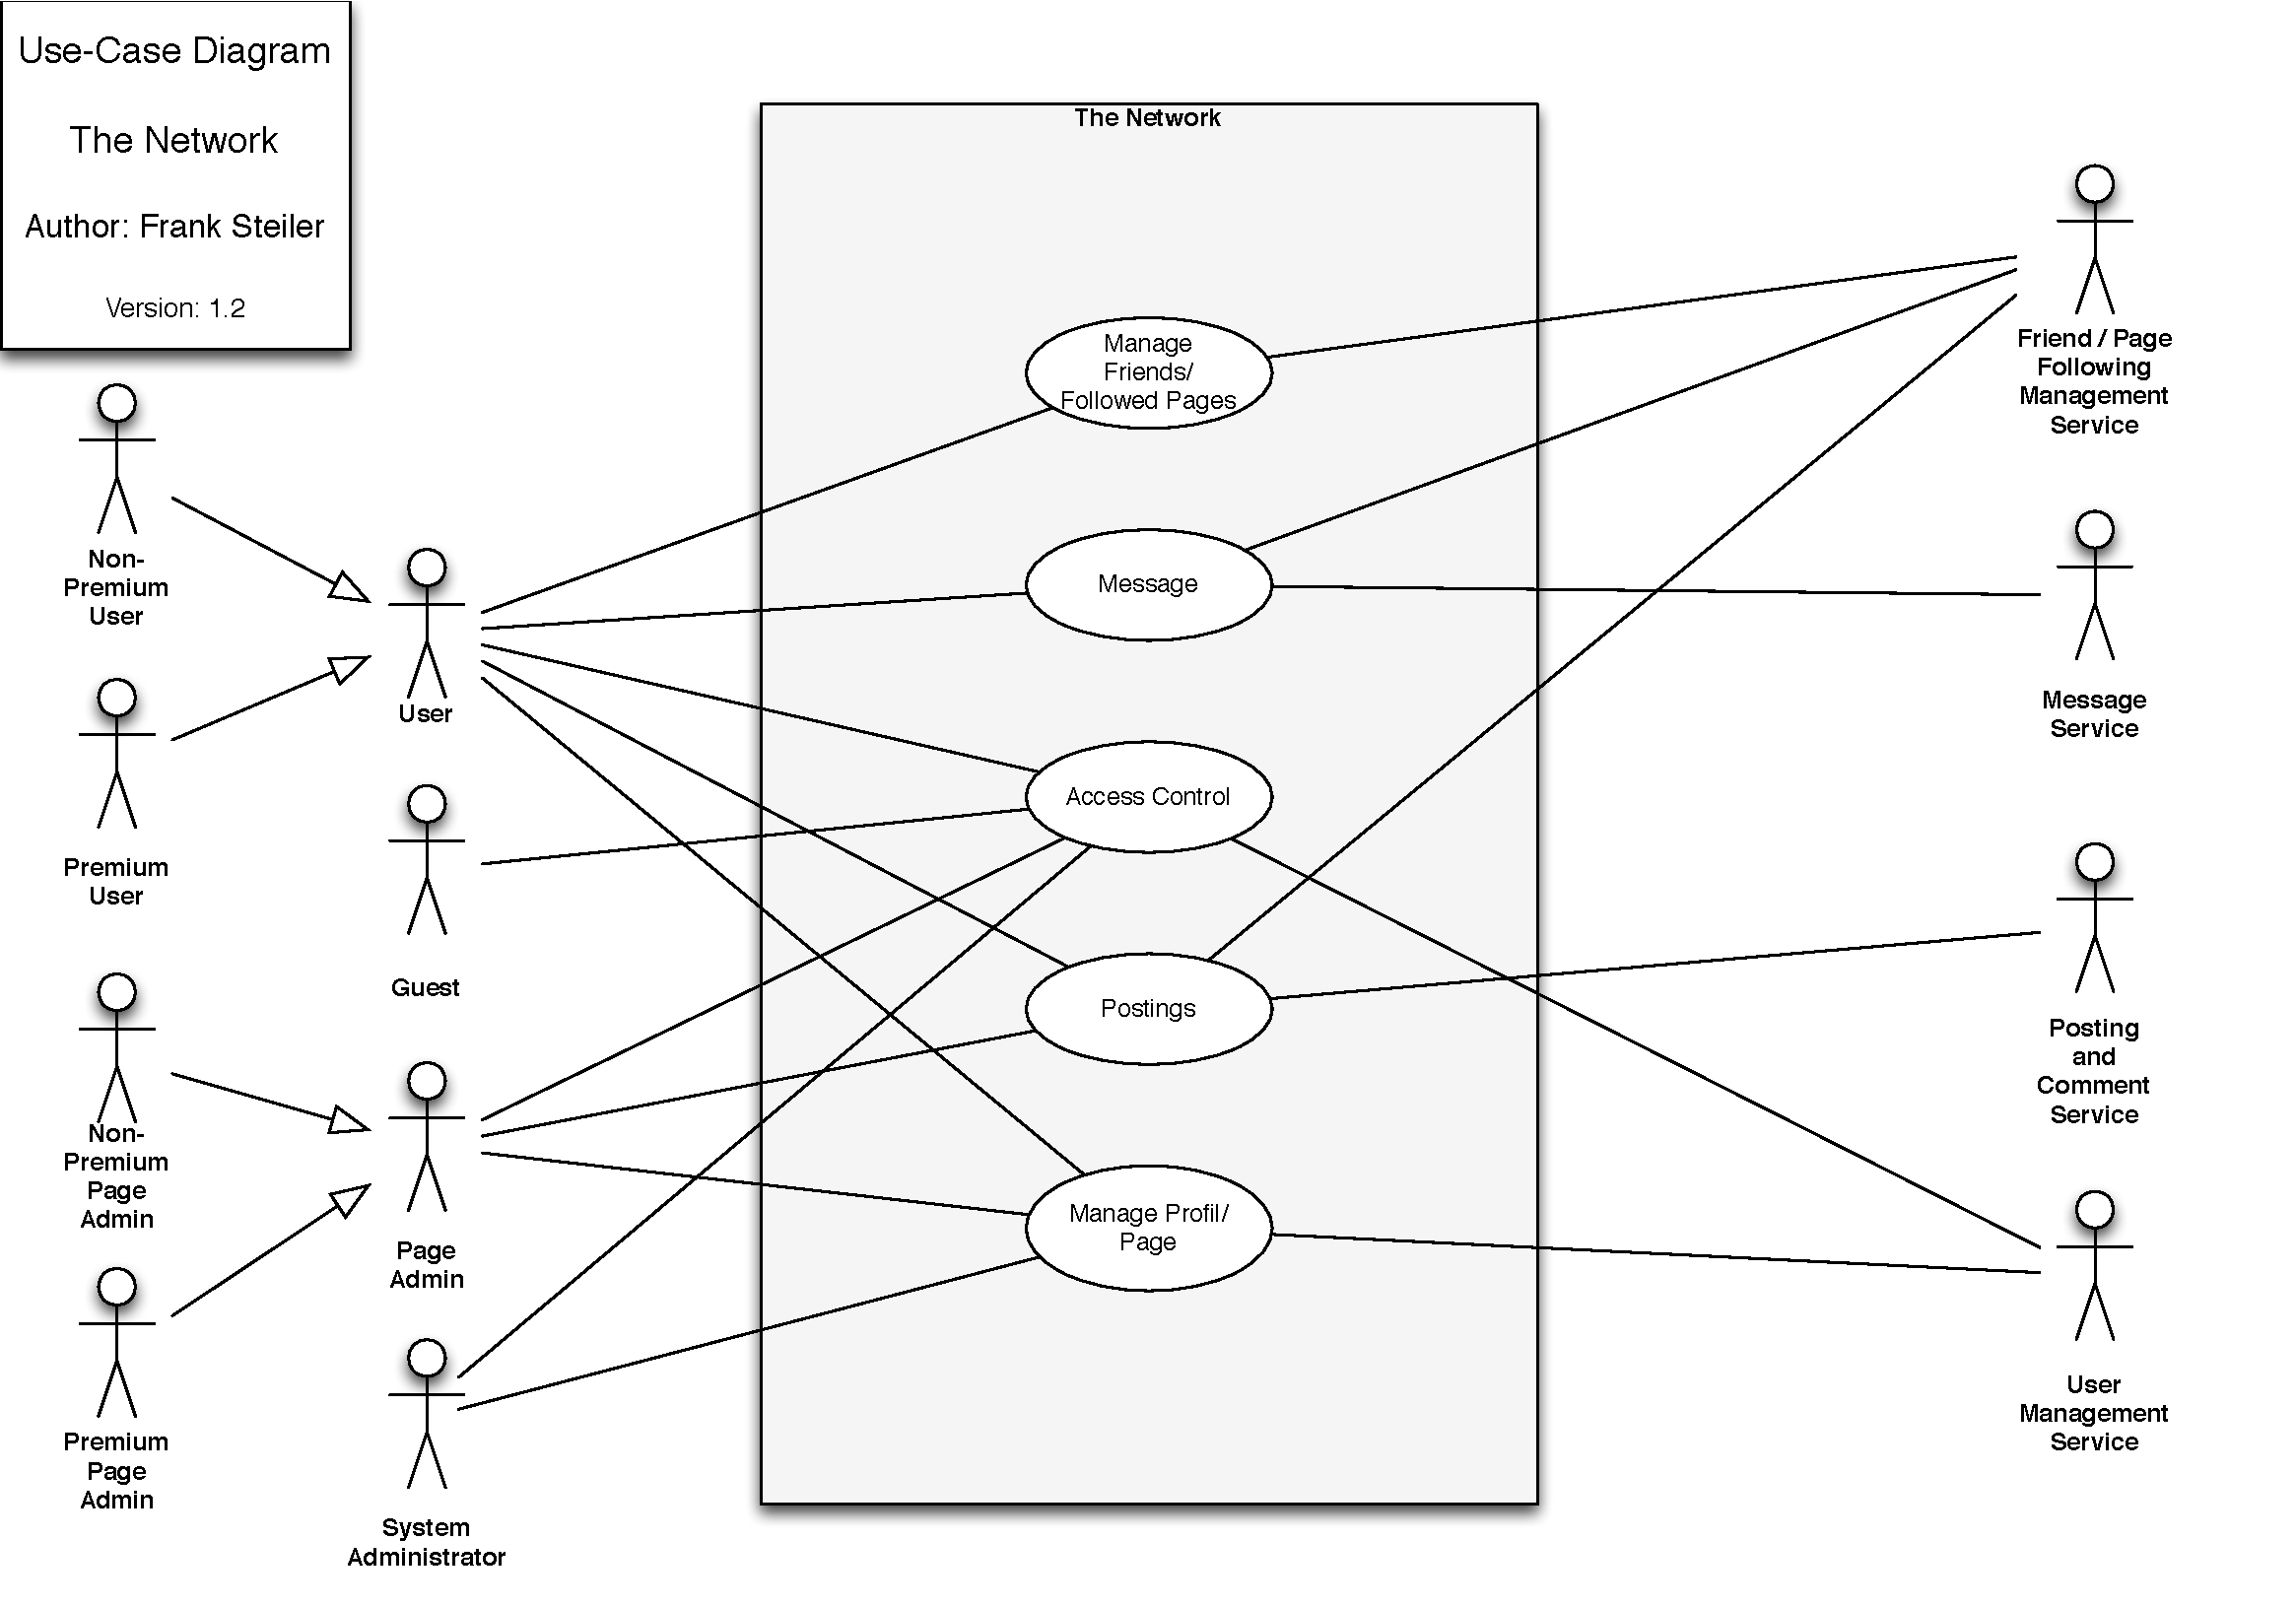
\includepdf[fitpaper=true,pages=-,addtotoc={1,chapter,0,Use-Case diagram -- Overview,app:Use-Case_Diagram_TheNetwork}]{./Appendix/Use-Case_Diagram_1_TheNetwork.pdf}
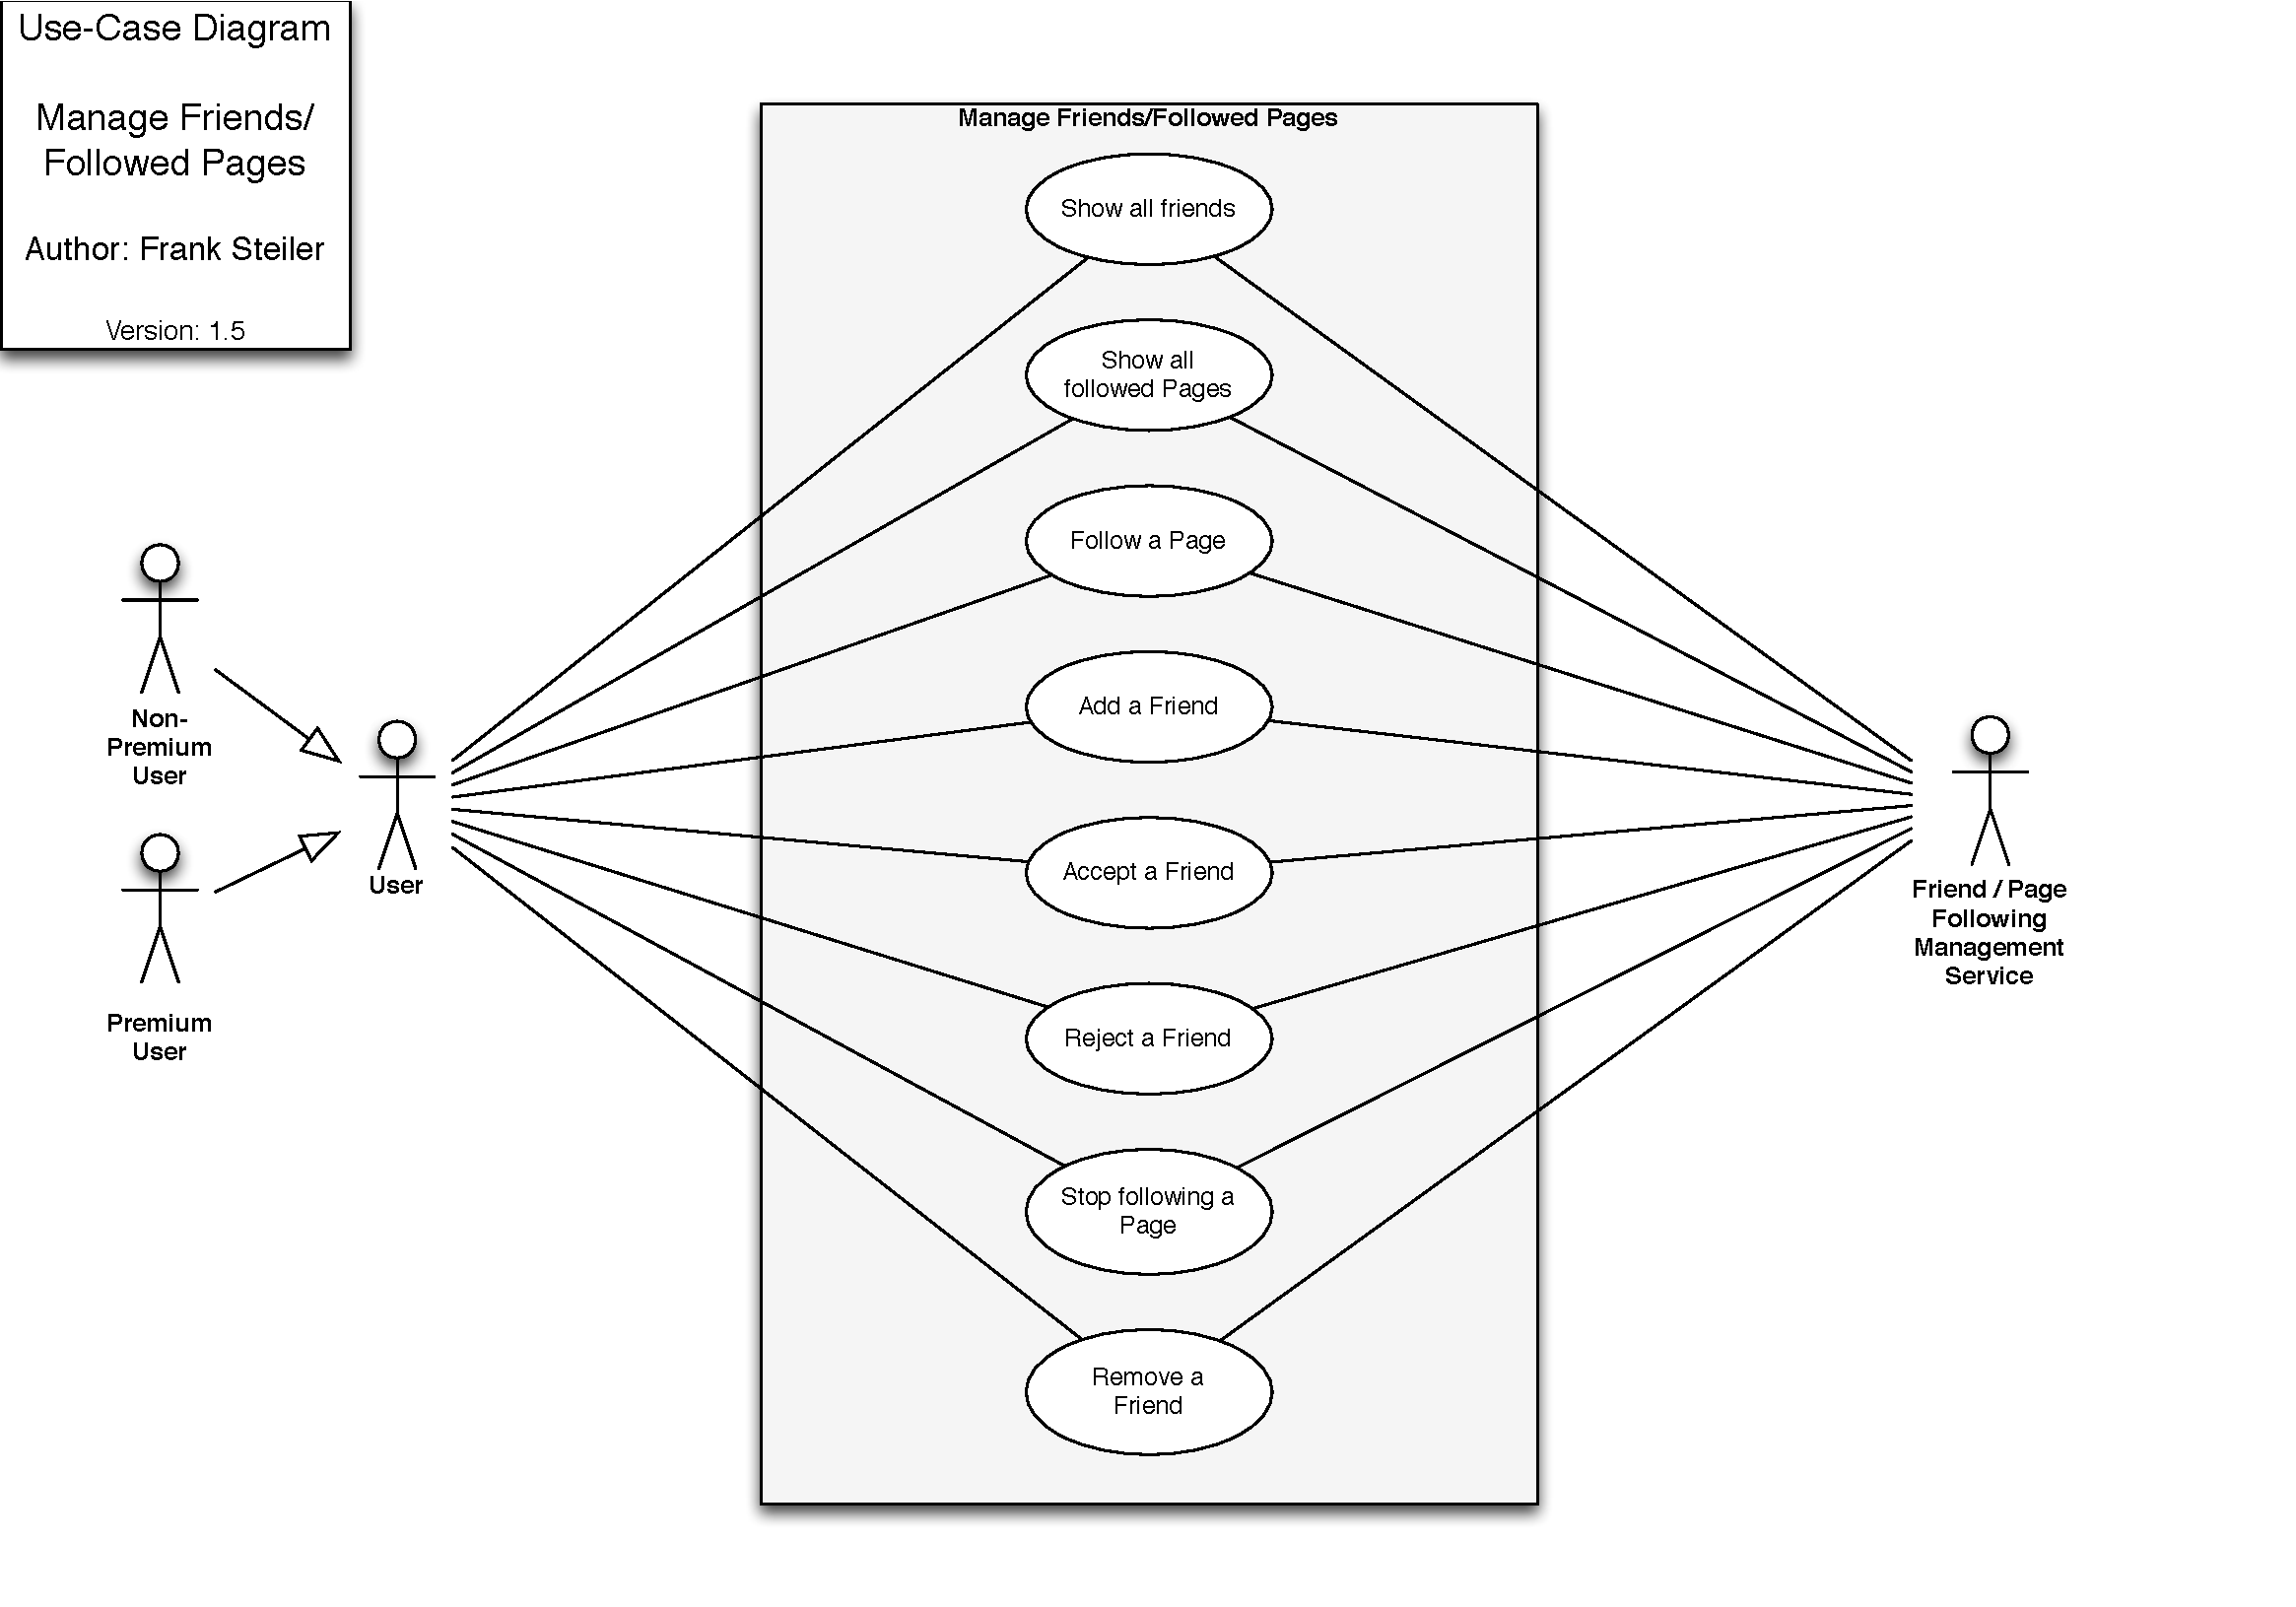
\includepdf[fitpaper=true,pages=-,addtotoc={1,section,1,Use-Case diagram -- Manage friends \& followed pages,app:Use-Case_Diagram_ManageFriends}]{./Appendix/Use-Case_Diagram_2_ManageFriends.pdf}
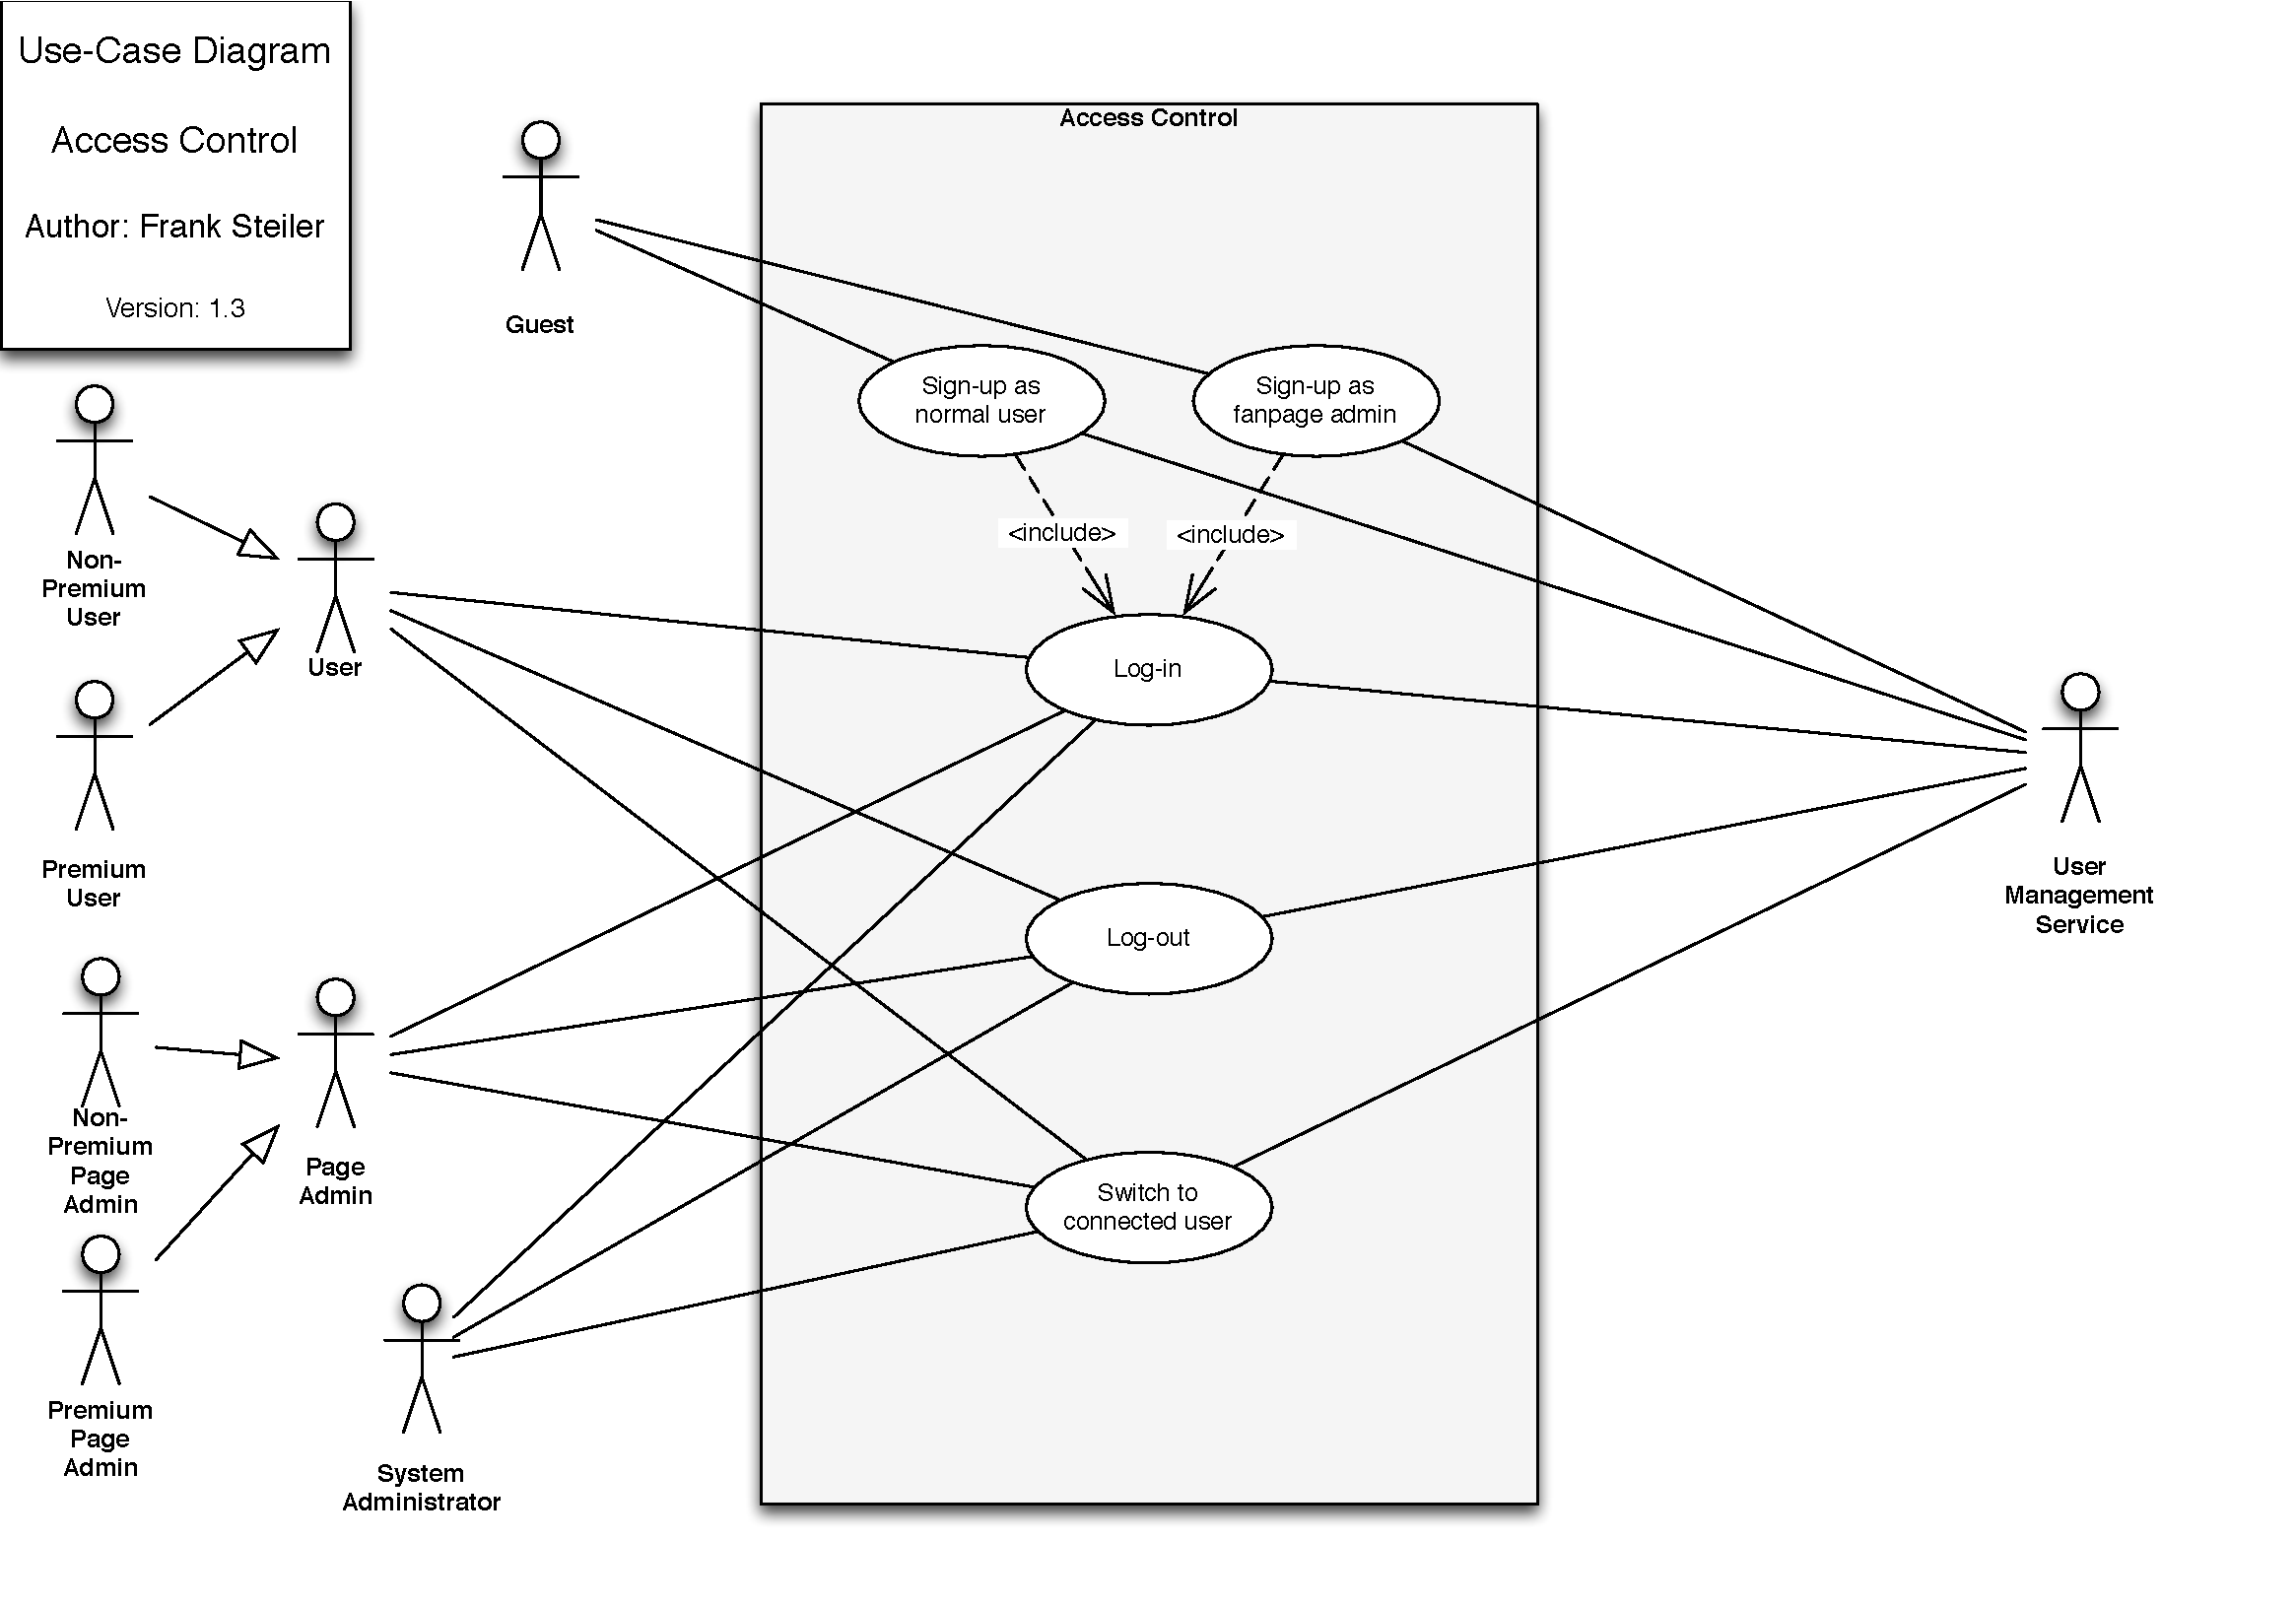
\includepdf[fitpaper=true,pages=-,addtotoc={1,section,1,Use-Case diagram -- Access Control,app:Use-Case_Diagram_Access_Control}]{./Appendix/Use-Case_Diagram_3_Access_Control.pdf}
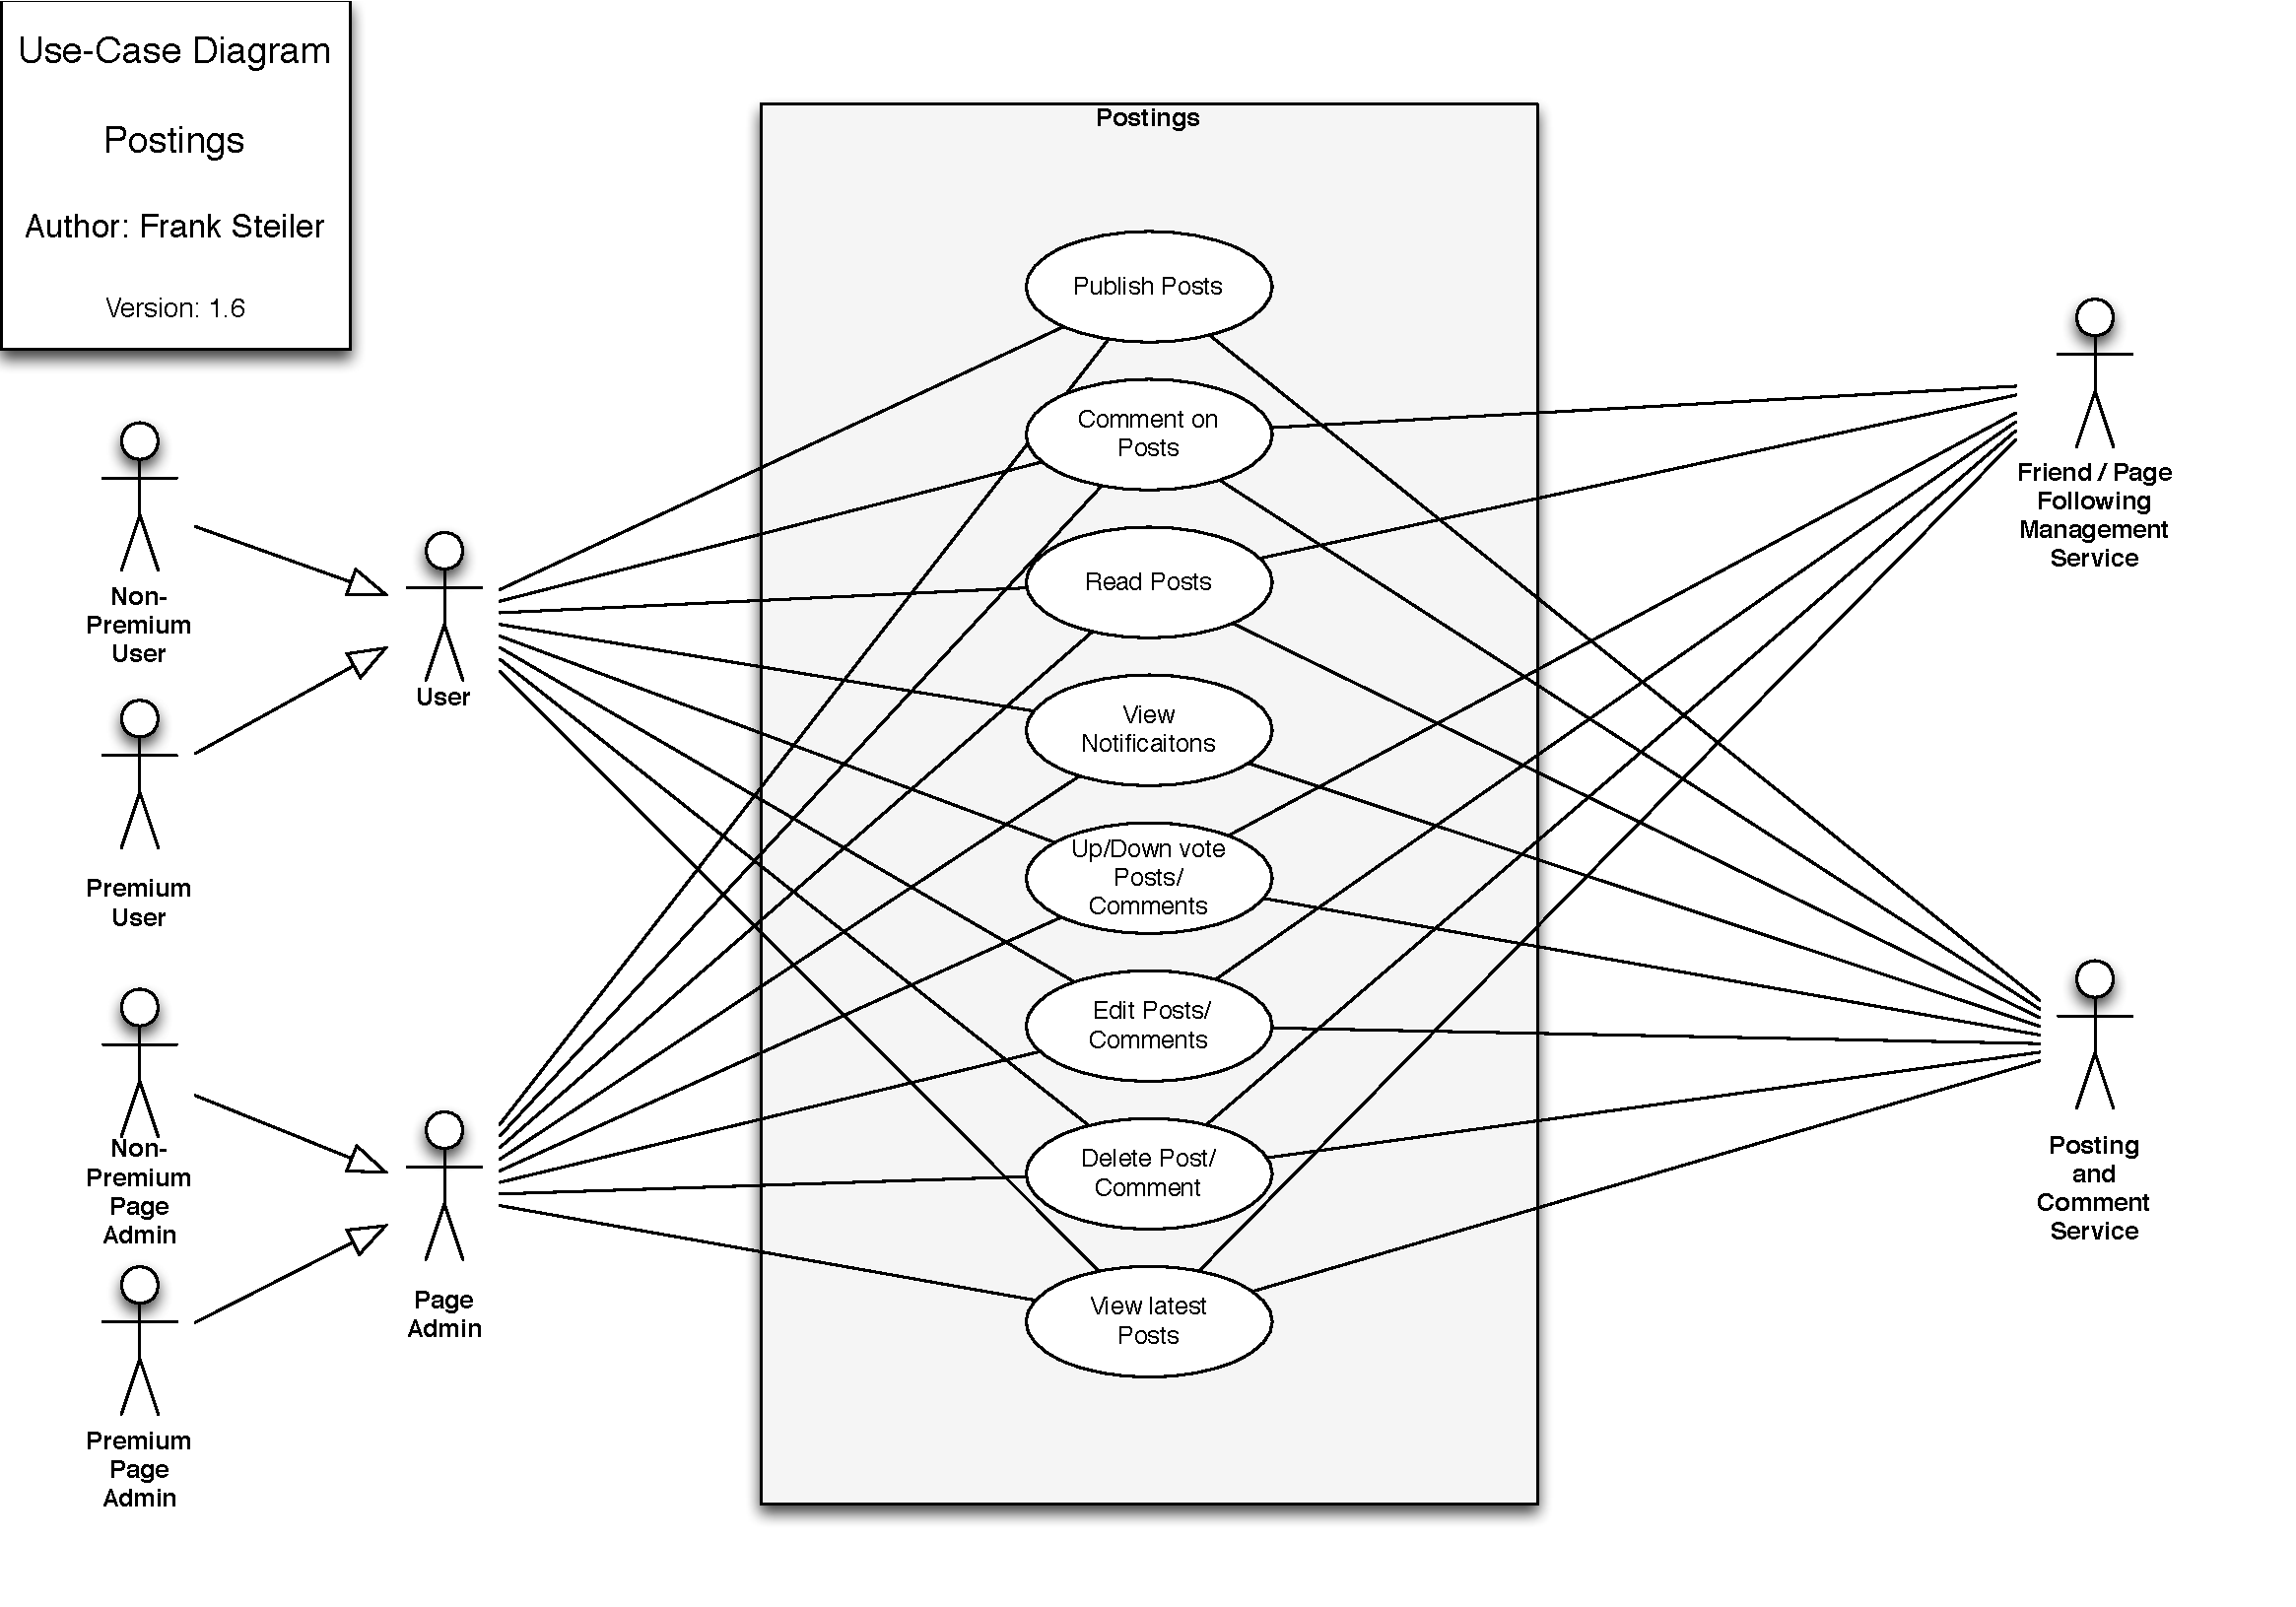
\includepdf[fitpaper=true,pages=-,addtotoc={1,section,1,Use-Case diagram -- Postings,app:Use-Case_Diagram_Postings}]{./Appendix/Use-Case_Diagram_4_Postings.pdf}
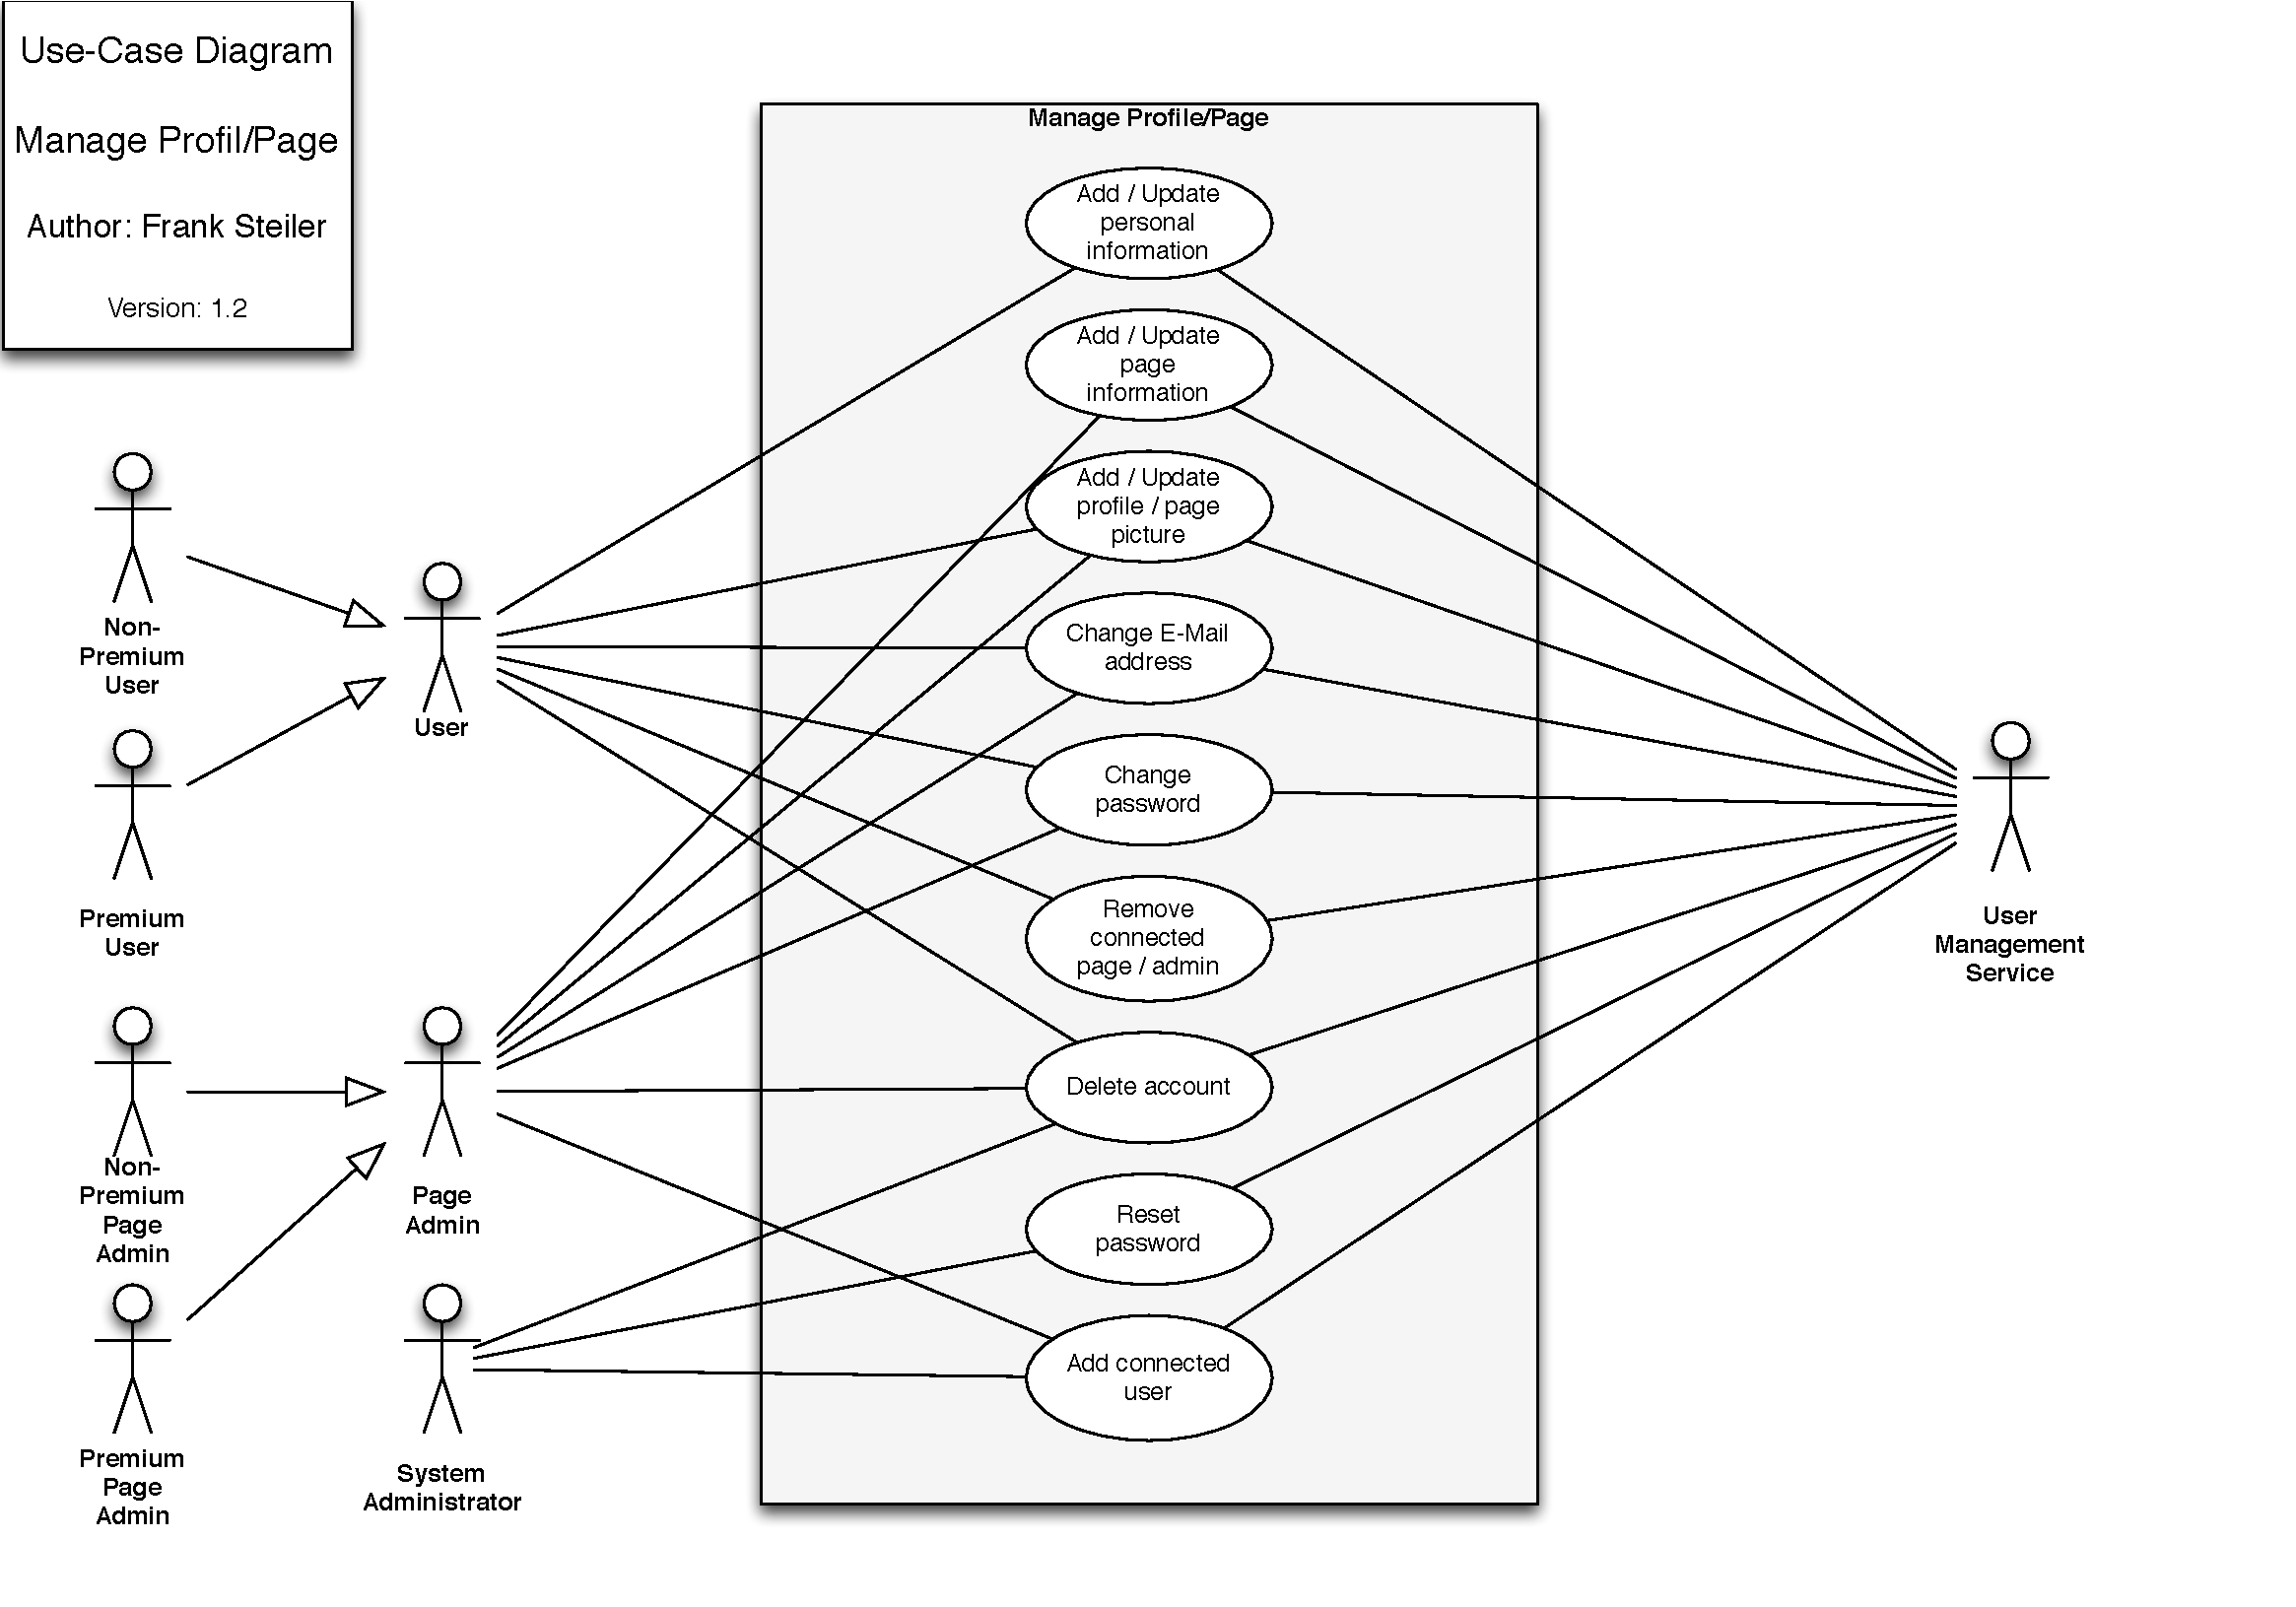
\includepdf[fitpaper=true,pages=-,addtotoc={1,section,1,Use-Case diagram -- Manage profile \& fanpage,app:Use-Case_Diagram_ManageProfil}]{./Appendix/Use-Case_Diagram_5_ManageProfile.pdf}
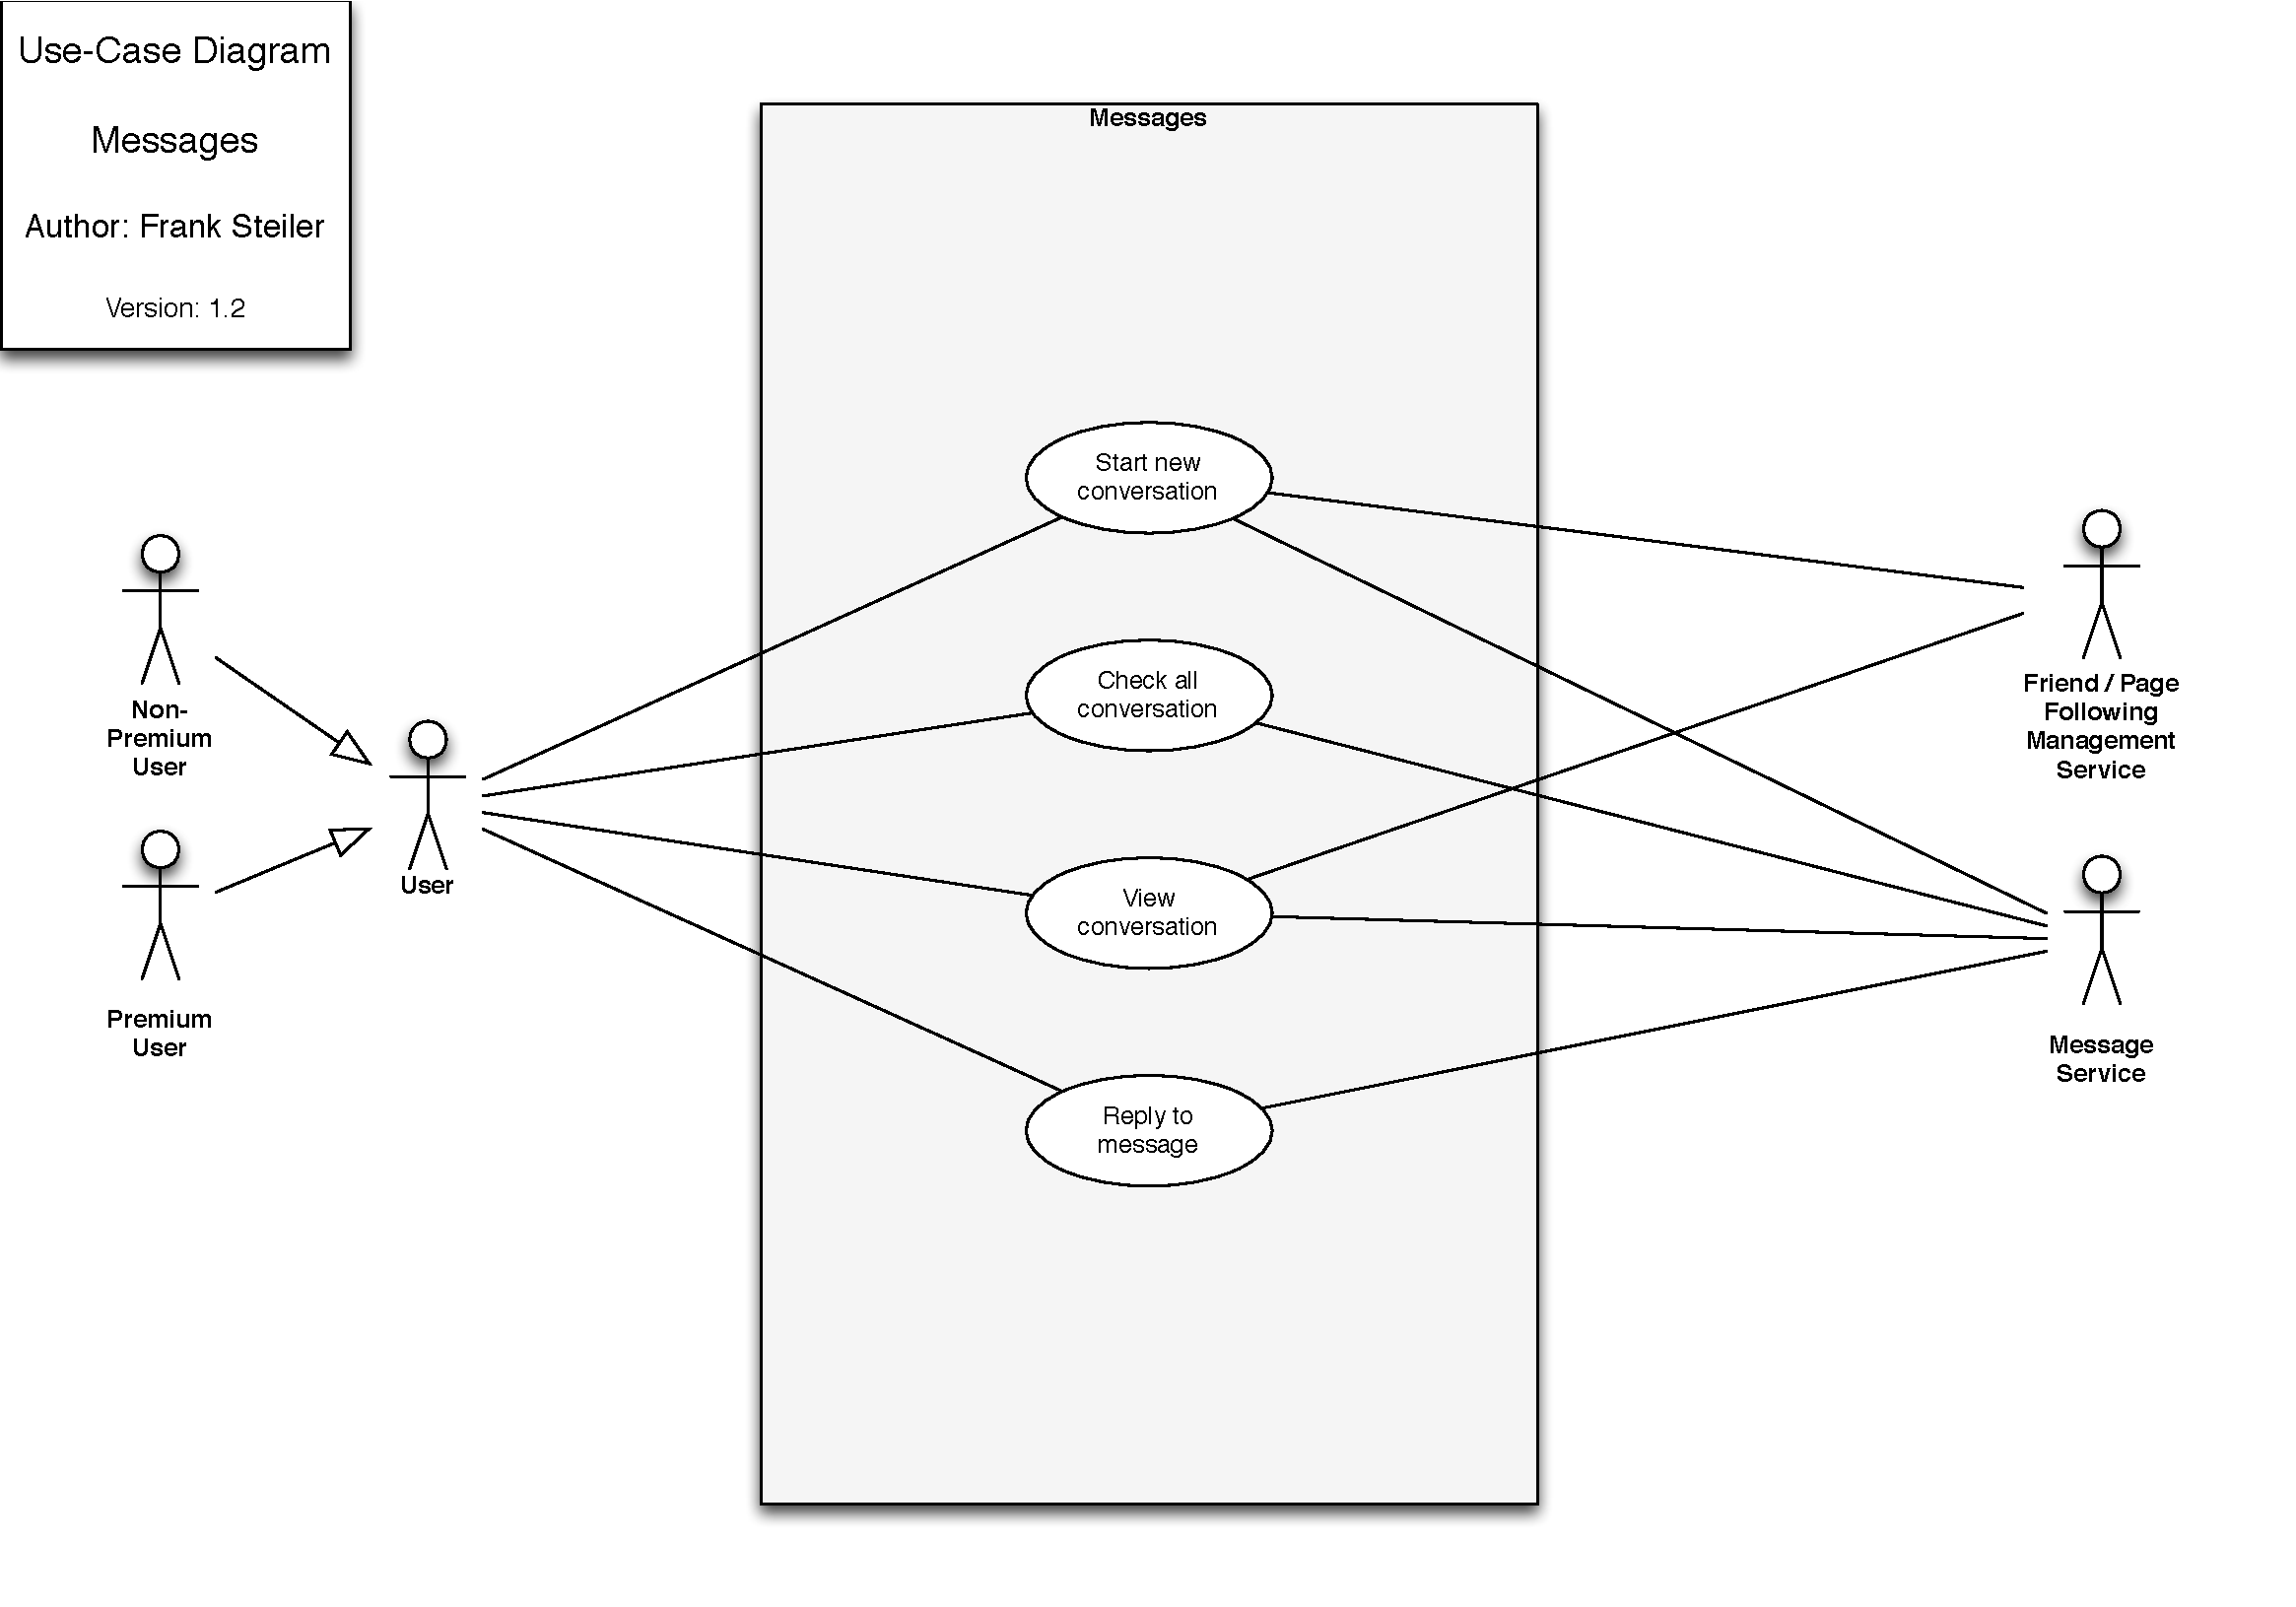
\includepdf[fitpaper=true,pages=-,addtotoc={1,section,1,Use-Case diagram -- Messages \& fanpage,app:Use-Case_Diagram_Messages}]{./Appendix/Use-Case_Diagram_6_Messages.pdf}

%UI/Page navigation
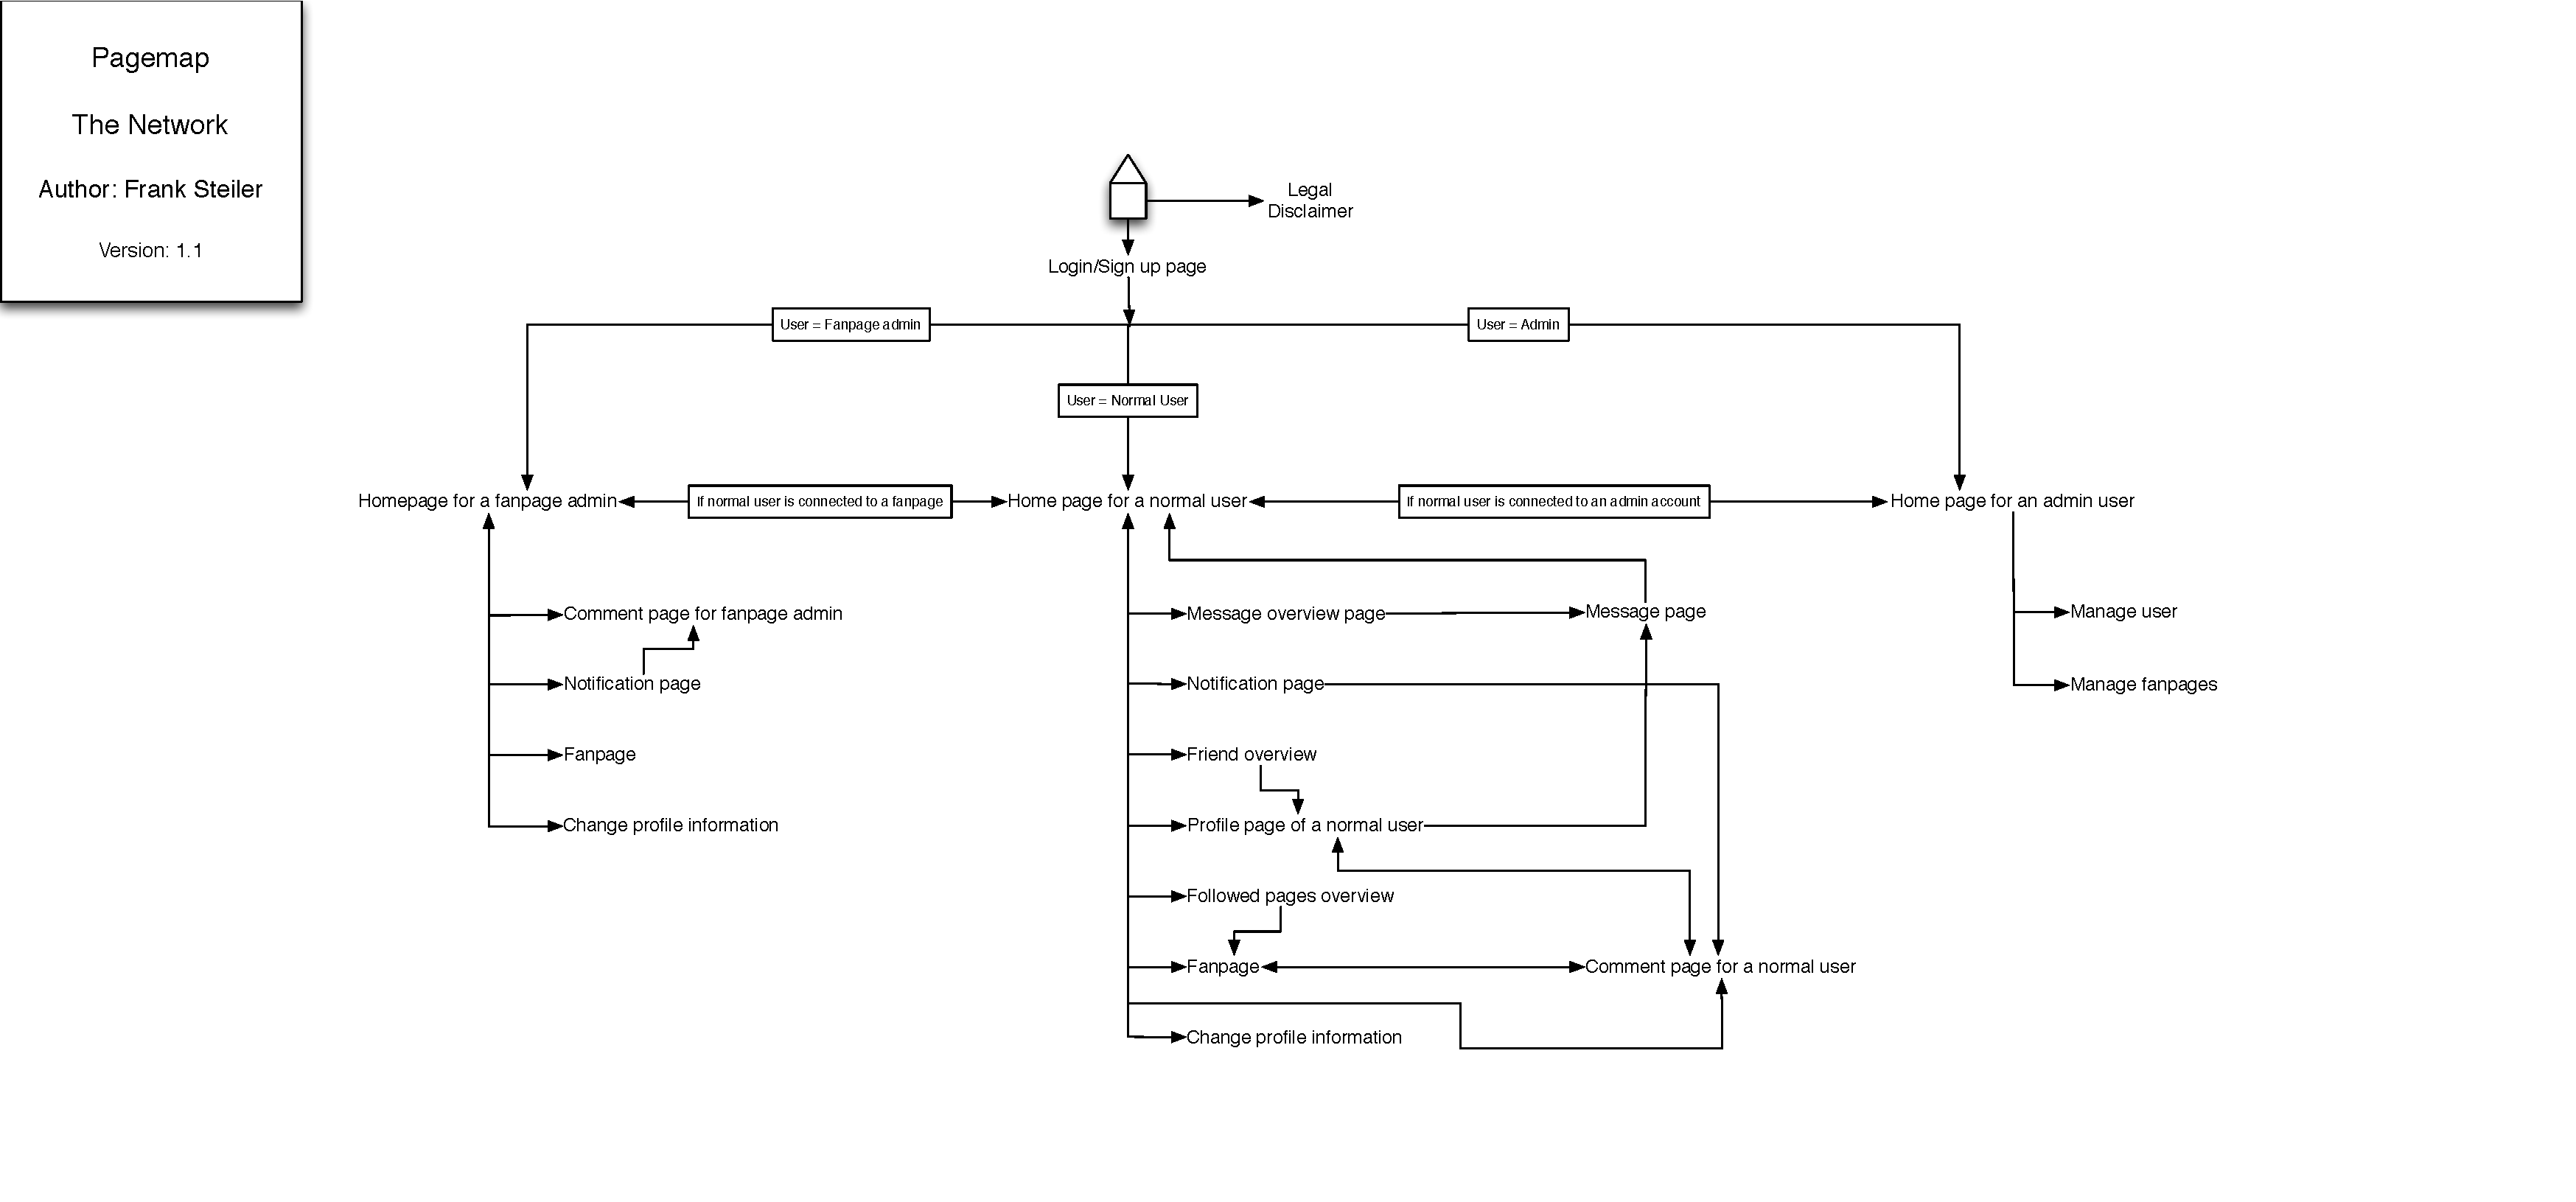
\includepdf[fitpaper=true,pages=-,addtotoc={1,chapter,0,Pagemap,app:Pagemap}]{./Appendix/Pagemap.pdf}
\includepdf[fitpaper=true,pages=-,addtotoc={1,chapter,0,Wireframes,app:Wireframes}]{./Appendix/WIreframes.pdf}

%Database
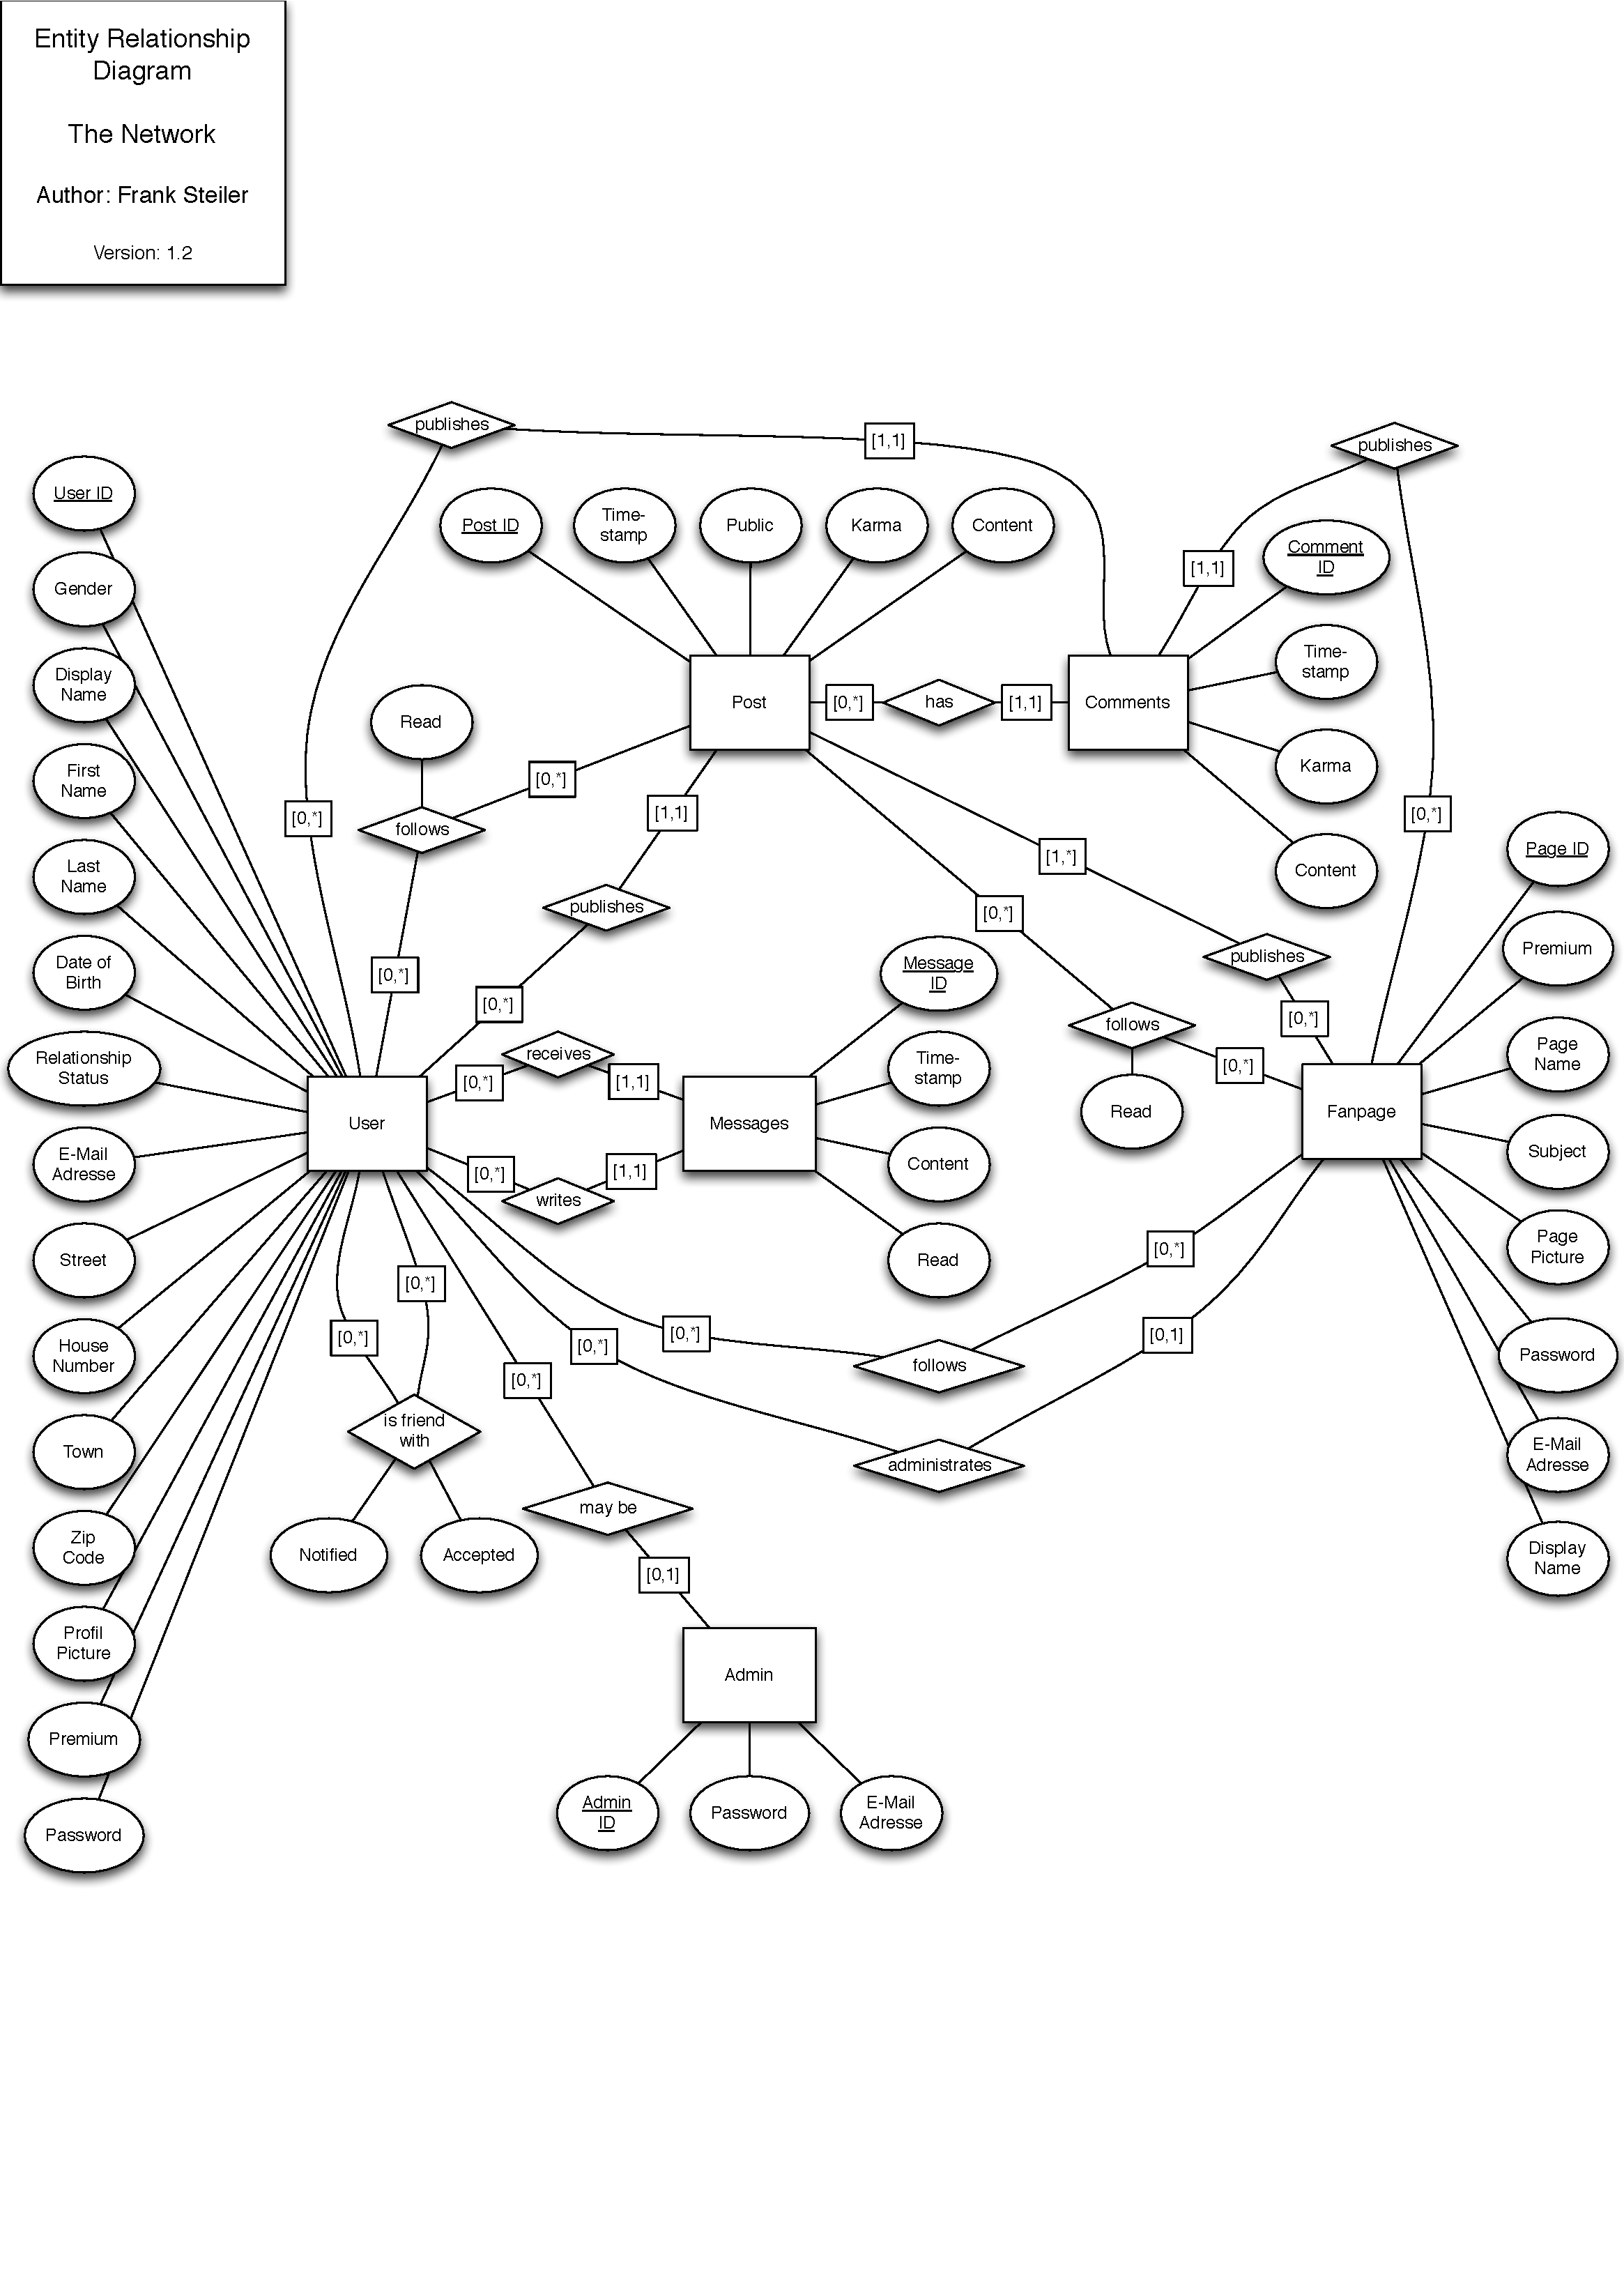
\includepdf[fitpaper=true,pages=-,addtotoc={1,chapter,0,ER-Model,app:ER-Model}]{./Appendix/ER-Model_Database.pdf}

%Component diagram
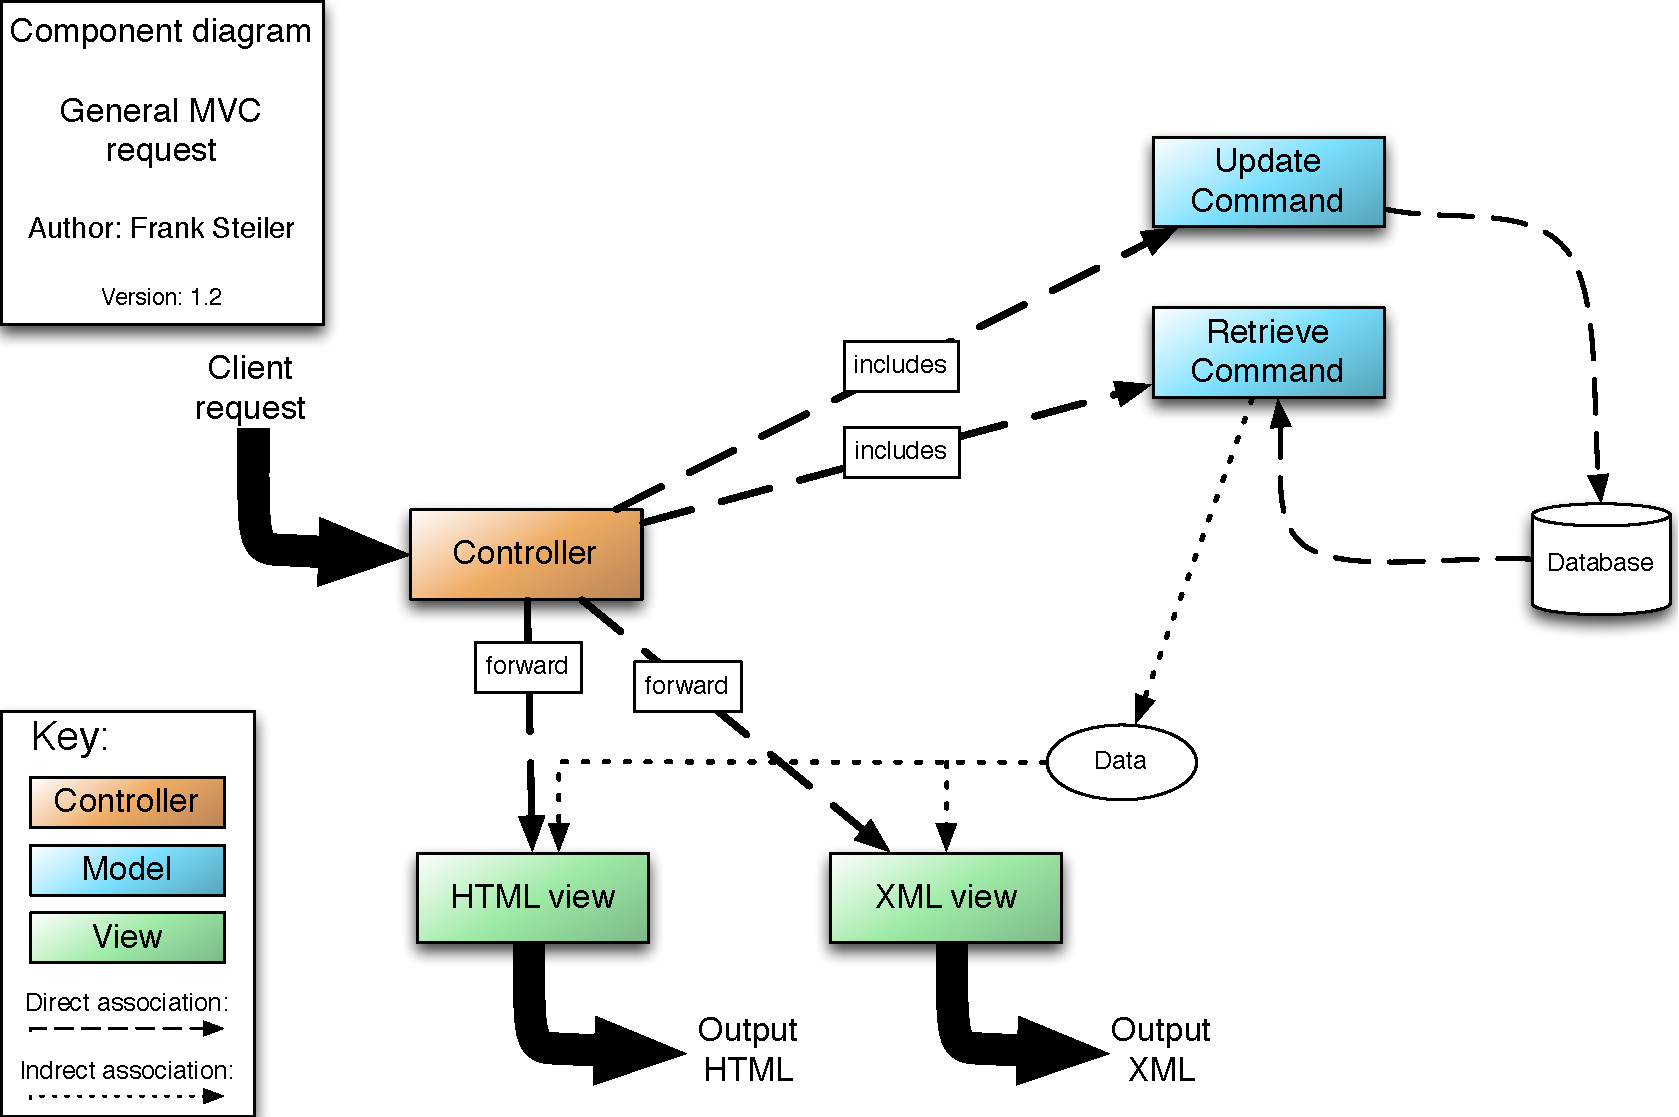
\includepdf[fitpaper=true,pages=-,addtotoc={1,chapter,0,Component diagram,app:ComponentDiagram}]{./Appendix/Component_diagram_General.pdf}
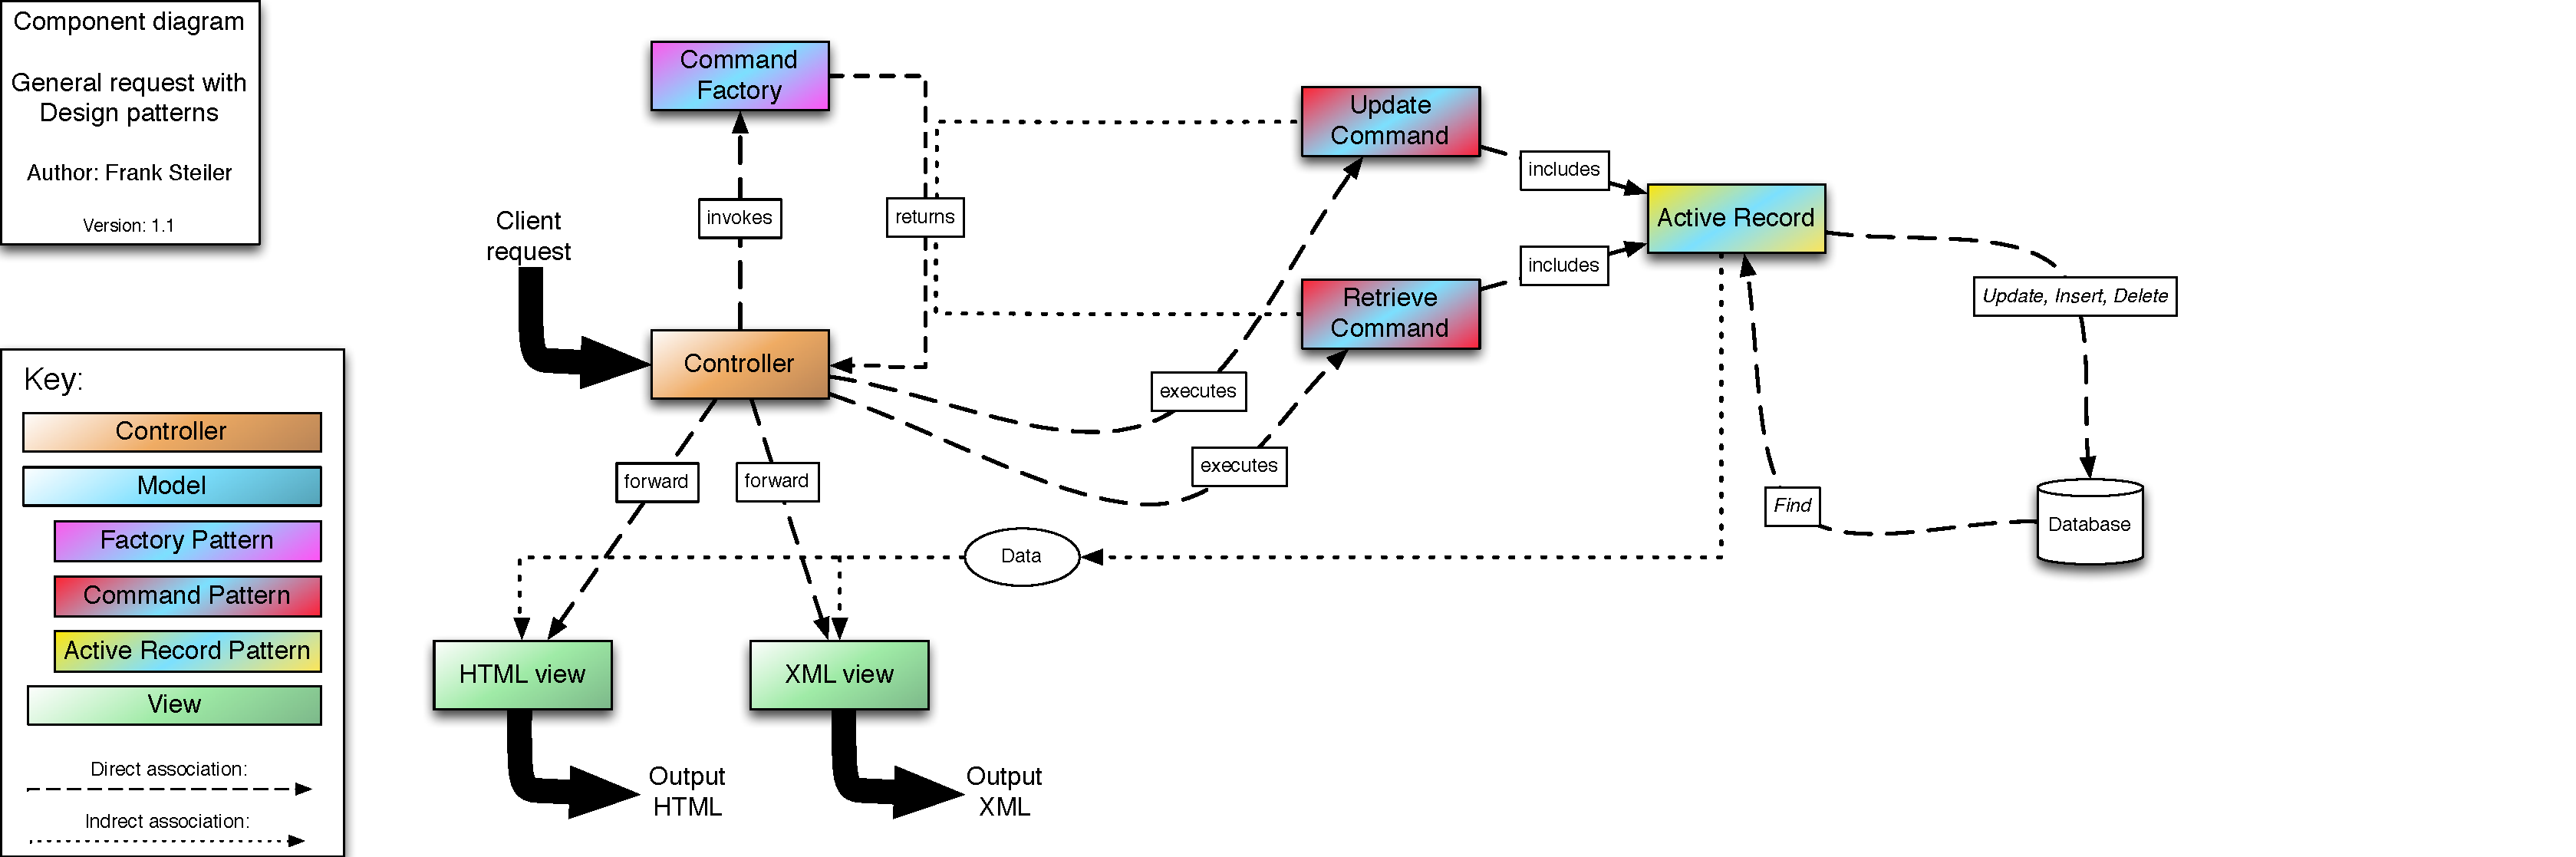
\includepdf[fitpaper=true,pages=-,addtotoc={1,section,1,Component diagram - General request with design patterns,app:ComponentDiagramPatterns}]{./Appendix/Component_diagram_General_Patterns.pdf}
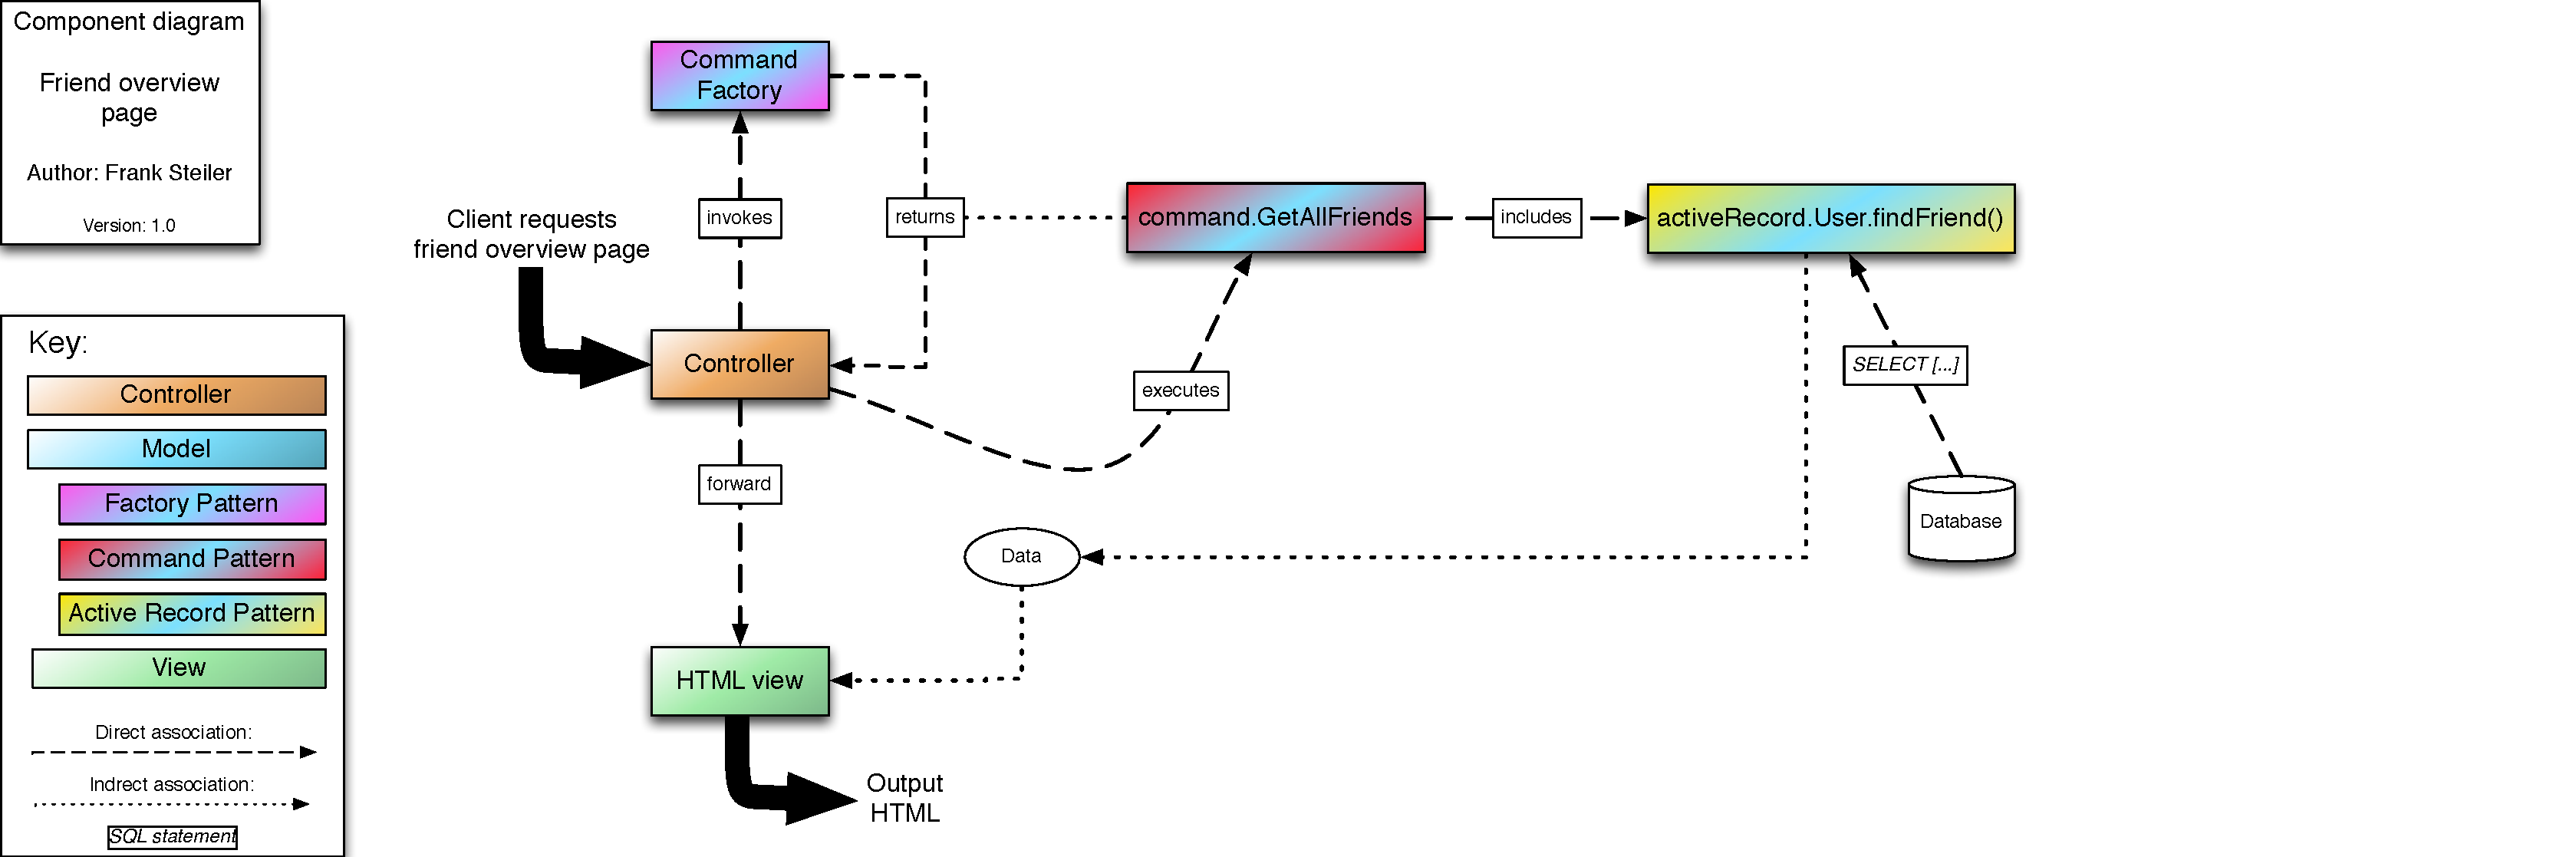
\includepdf[fitpaper=true,pages=-,addtotoc={1,section,1,Component diagram - Friend overview page,app:ComponentFriendOverview}]{./Appendix/Component_diagram_GetFriends.pdf}
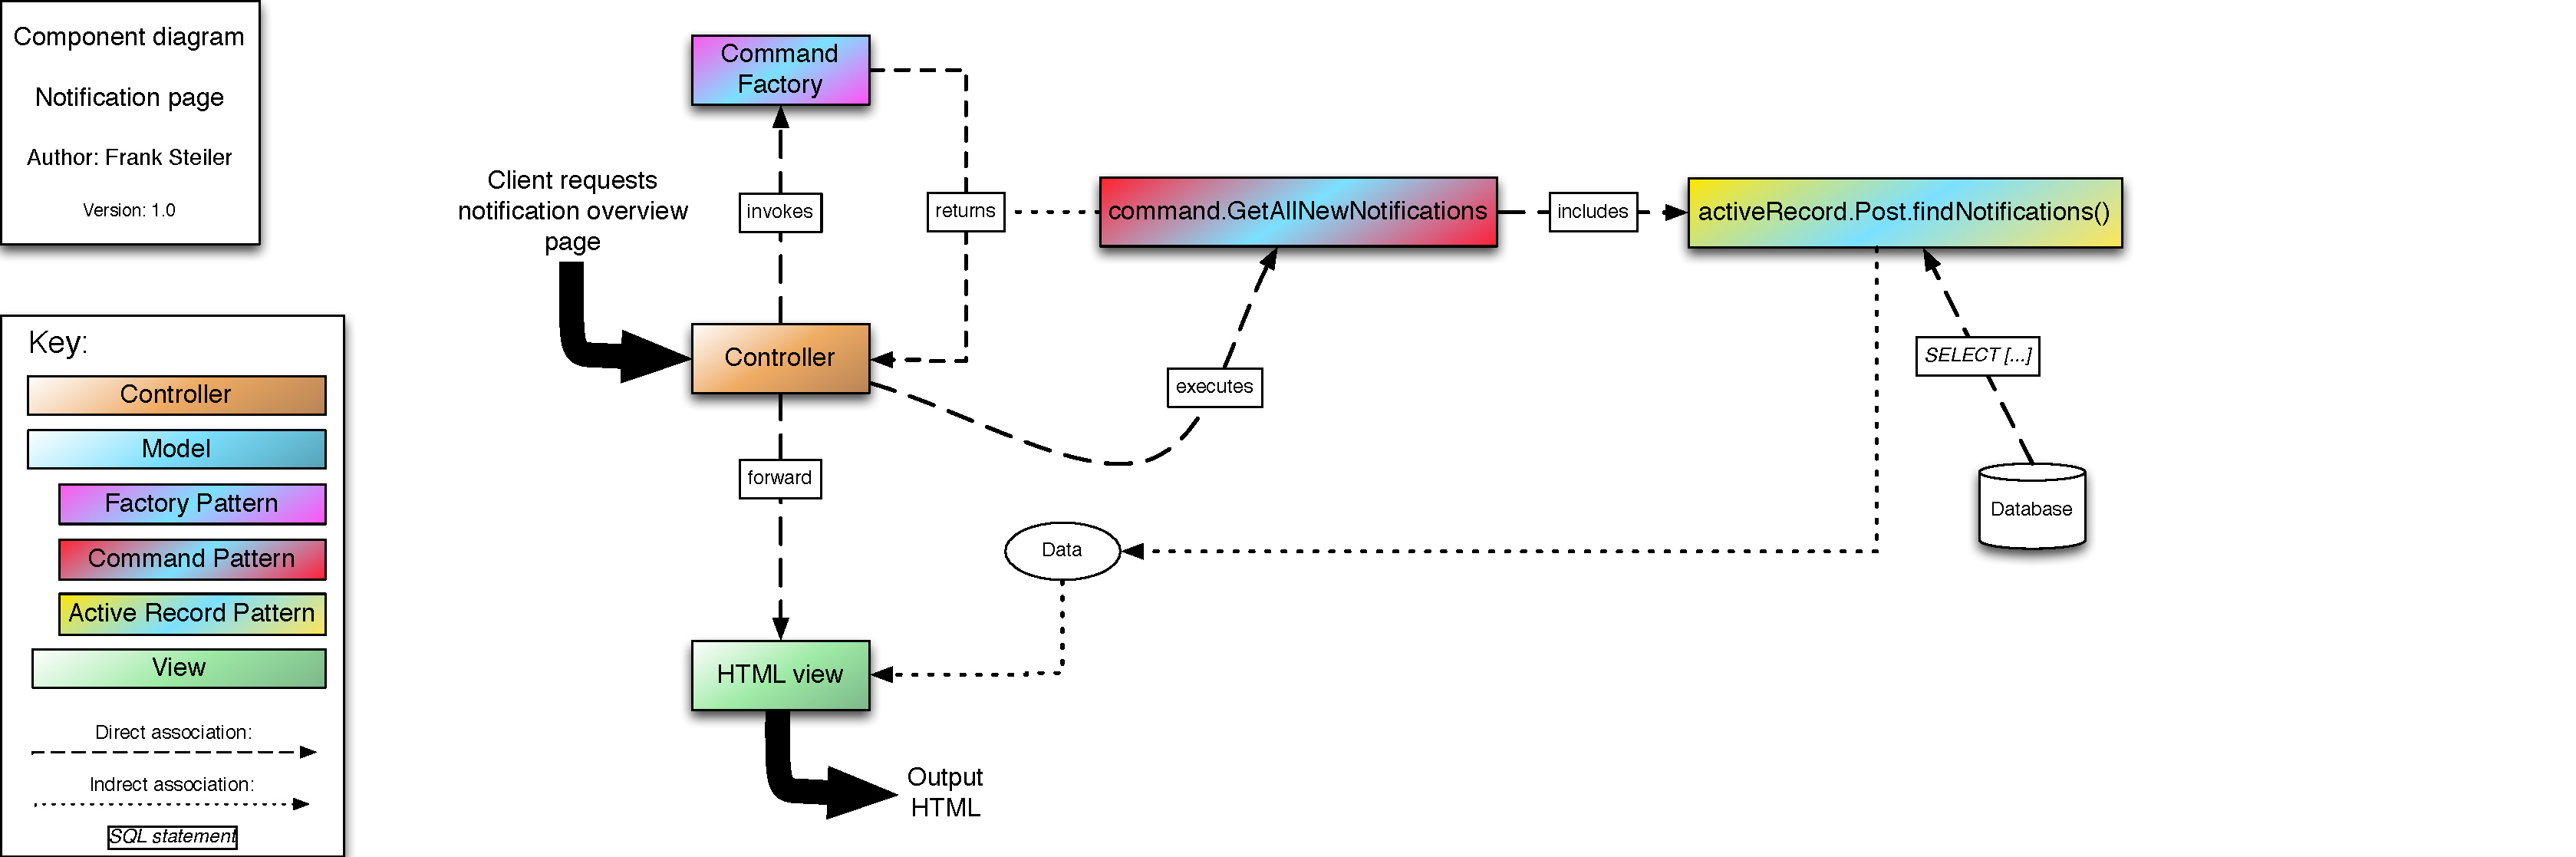
\includepdf[fitpaper=true,pages=-,addtotoc={1,section,1,Component diagram - Notification overview page,app:ComponentNotificationOverview}]{./Appendix/Component_diagram_GetNotifications.pdf}
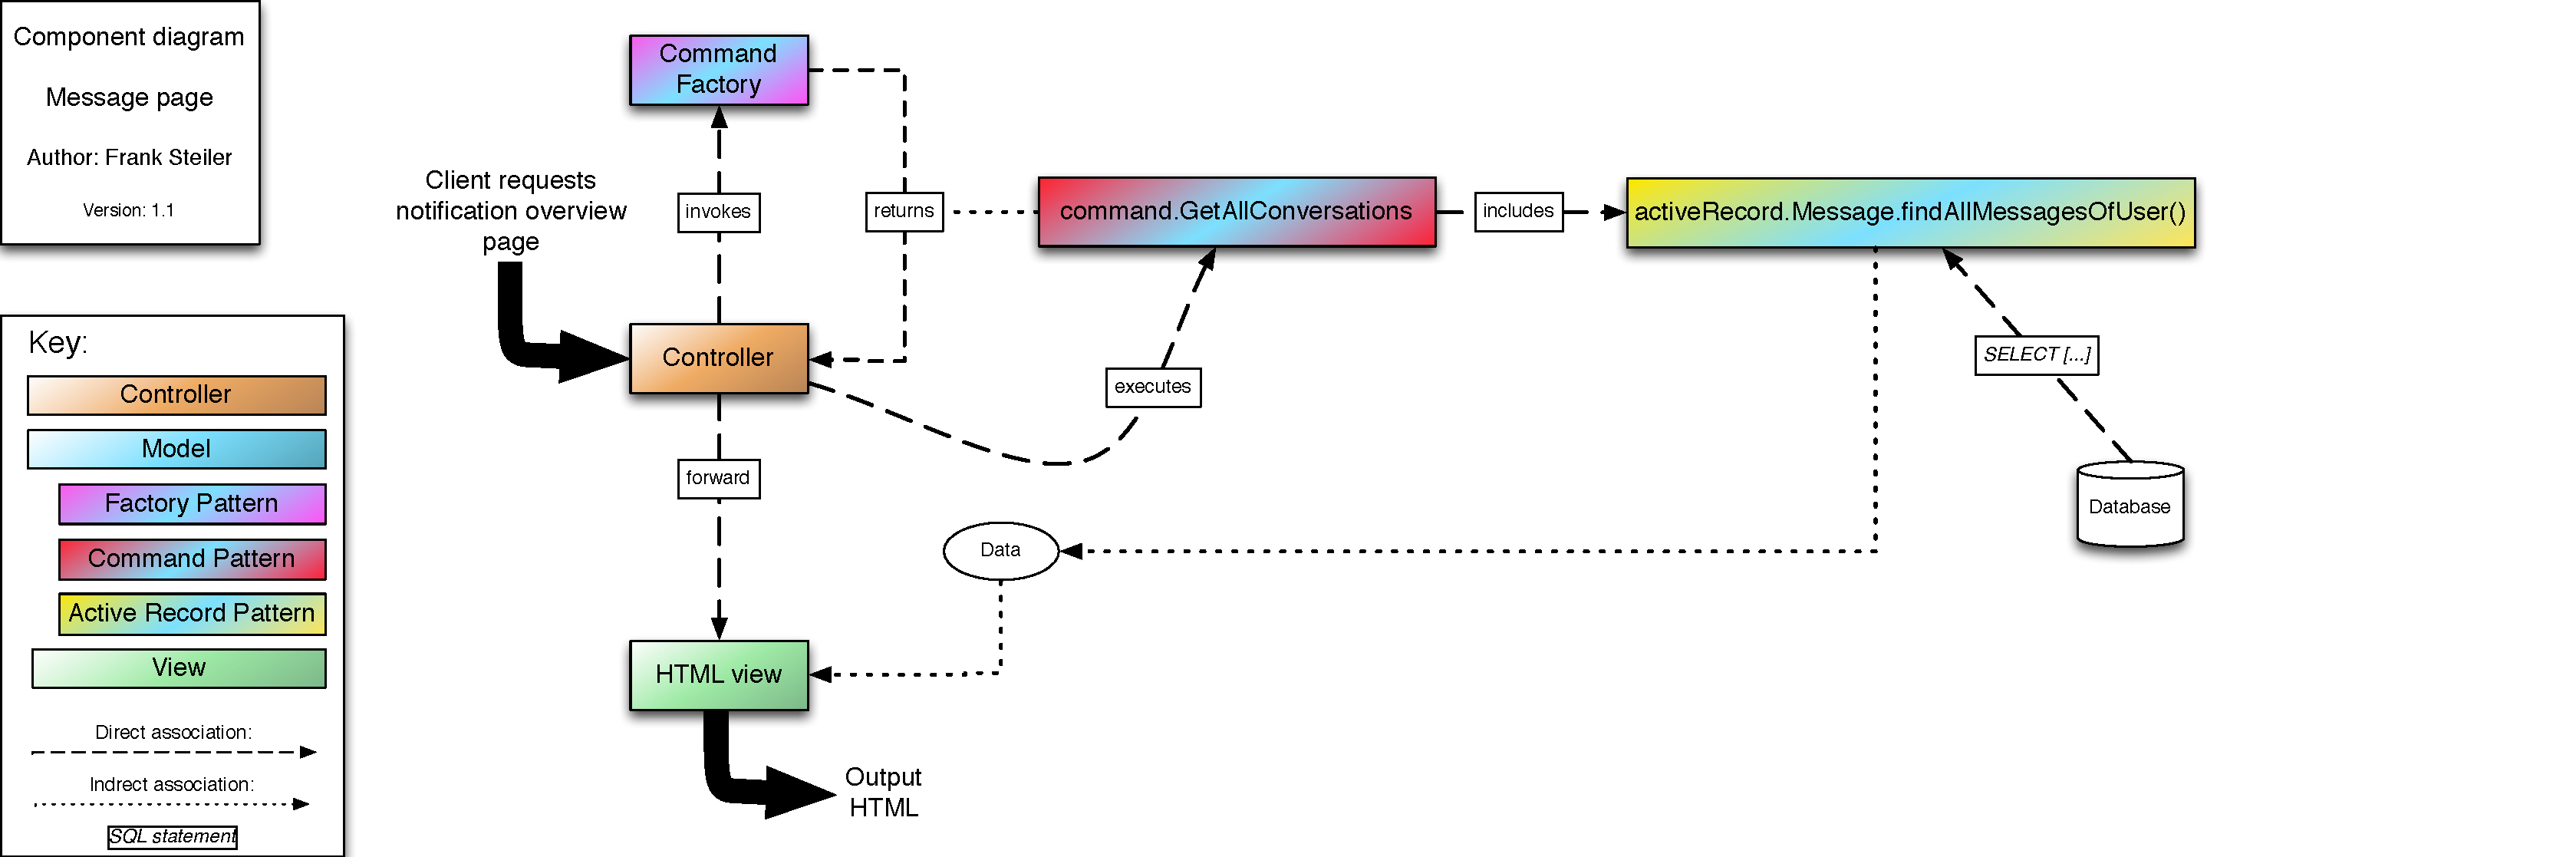
\includepdf[fitpaper=true,pages=-,addtotoc={1,section,1,Component diagram - Conversation overview page,app:ComponentConversationOverview}]{./Appendix/Component_diagram_GetConversations.pdf}
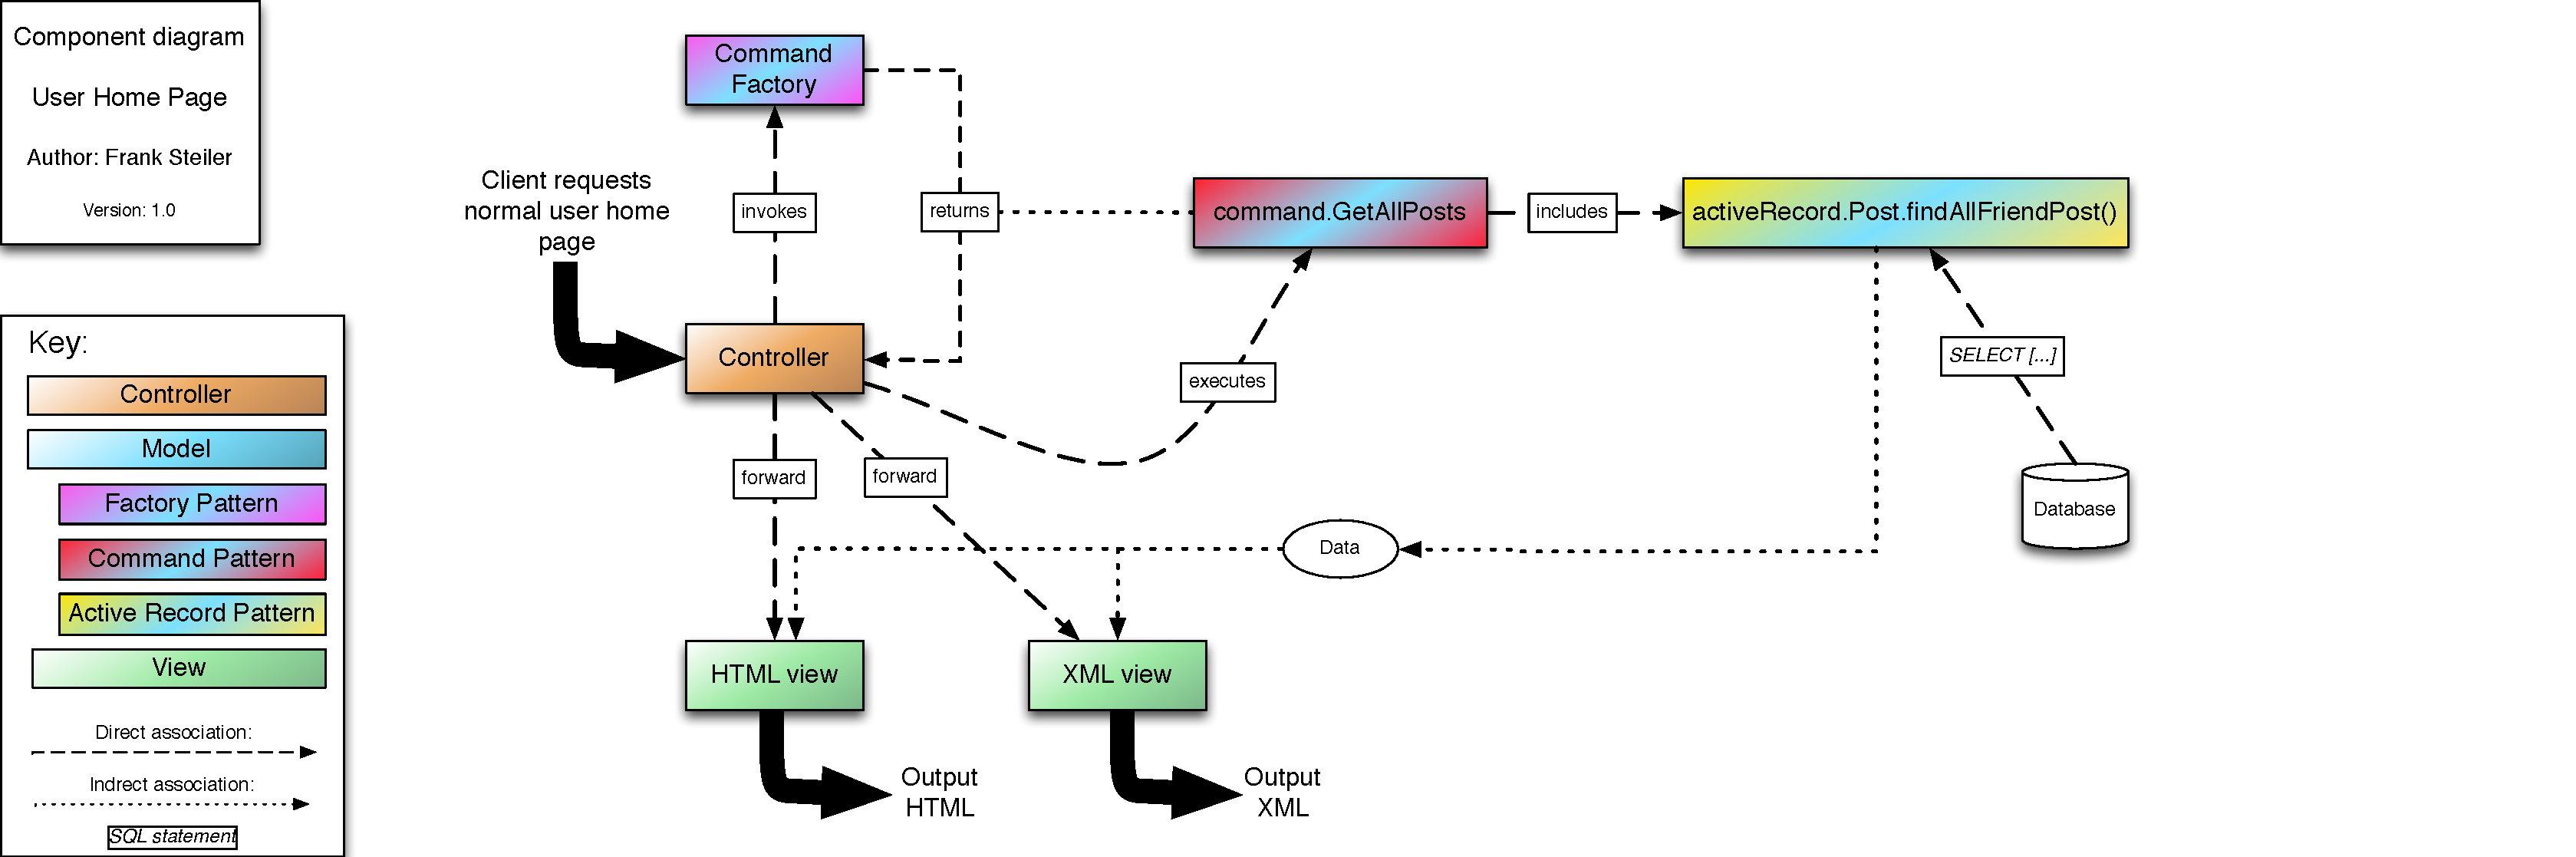
\includepdf[fitpaper=true,pages=-,addtotoc={1,section,1,Component diagram - Normal user home page,app:ComponentGetPosts}]{./Appendix/Component_diagram_GetPosts.pdf}
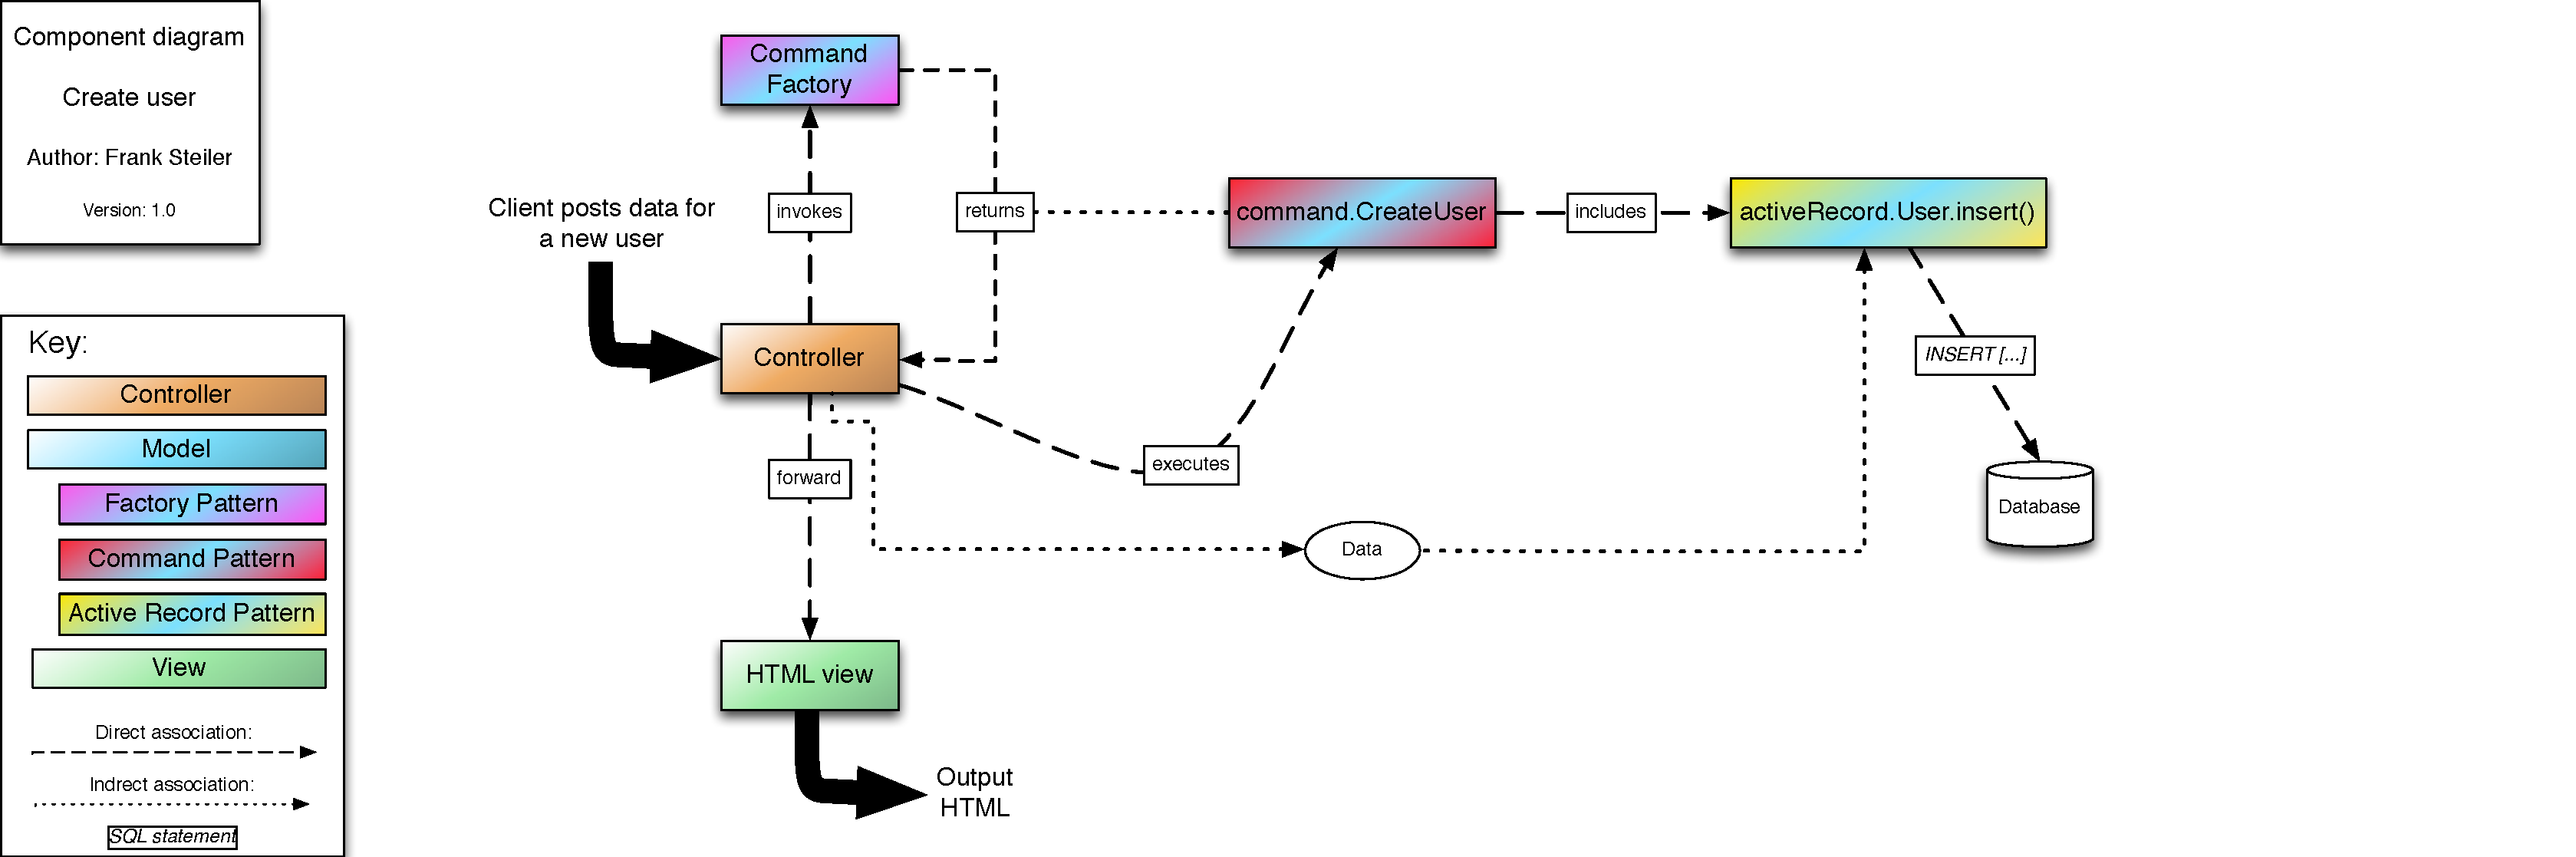
\includepdf[fitpaper=true,pages=-,addtotoc={1,section,1,Component diagram - Create User,app:ComponentCreateUser}]{./Appendix/Component_diagram_CreateUser.pdf}
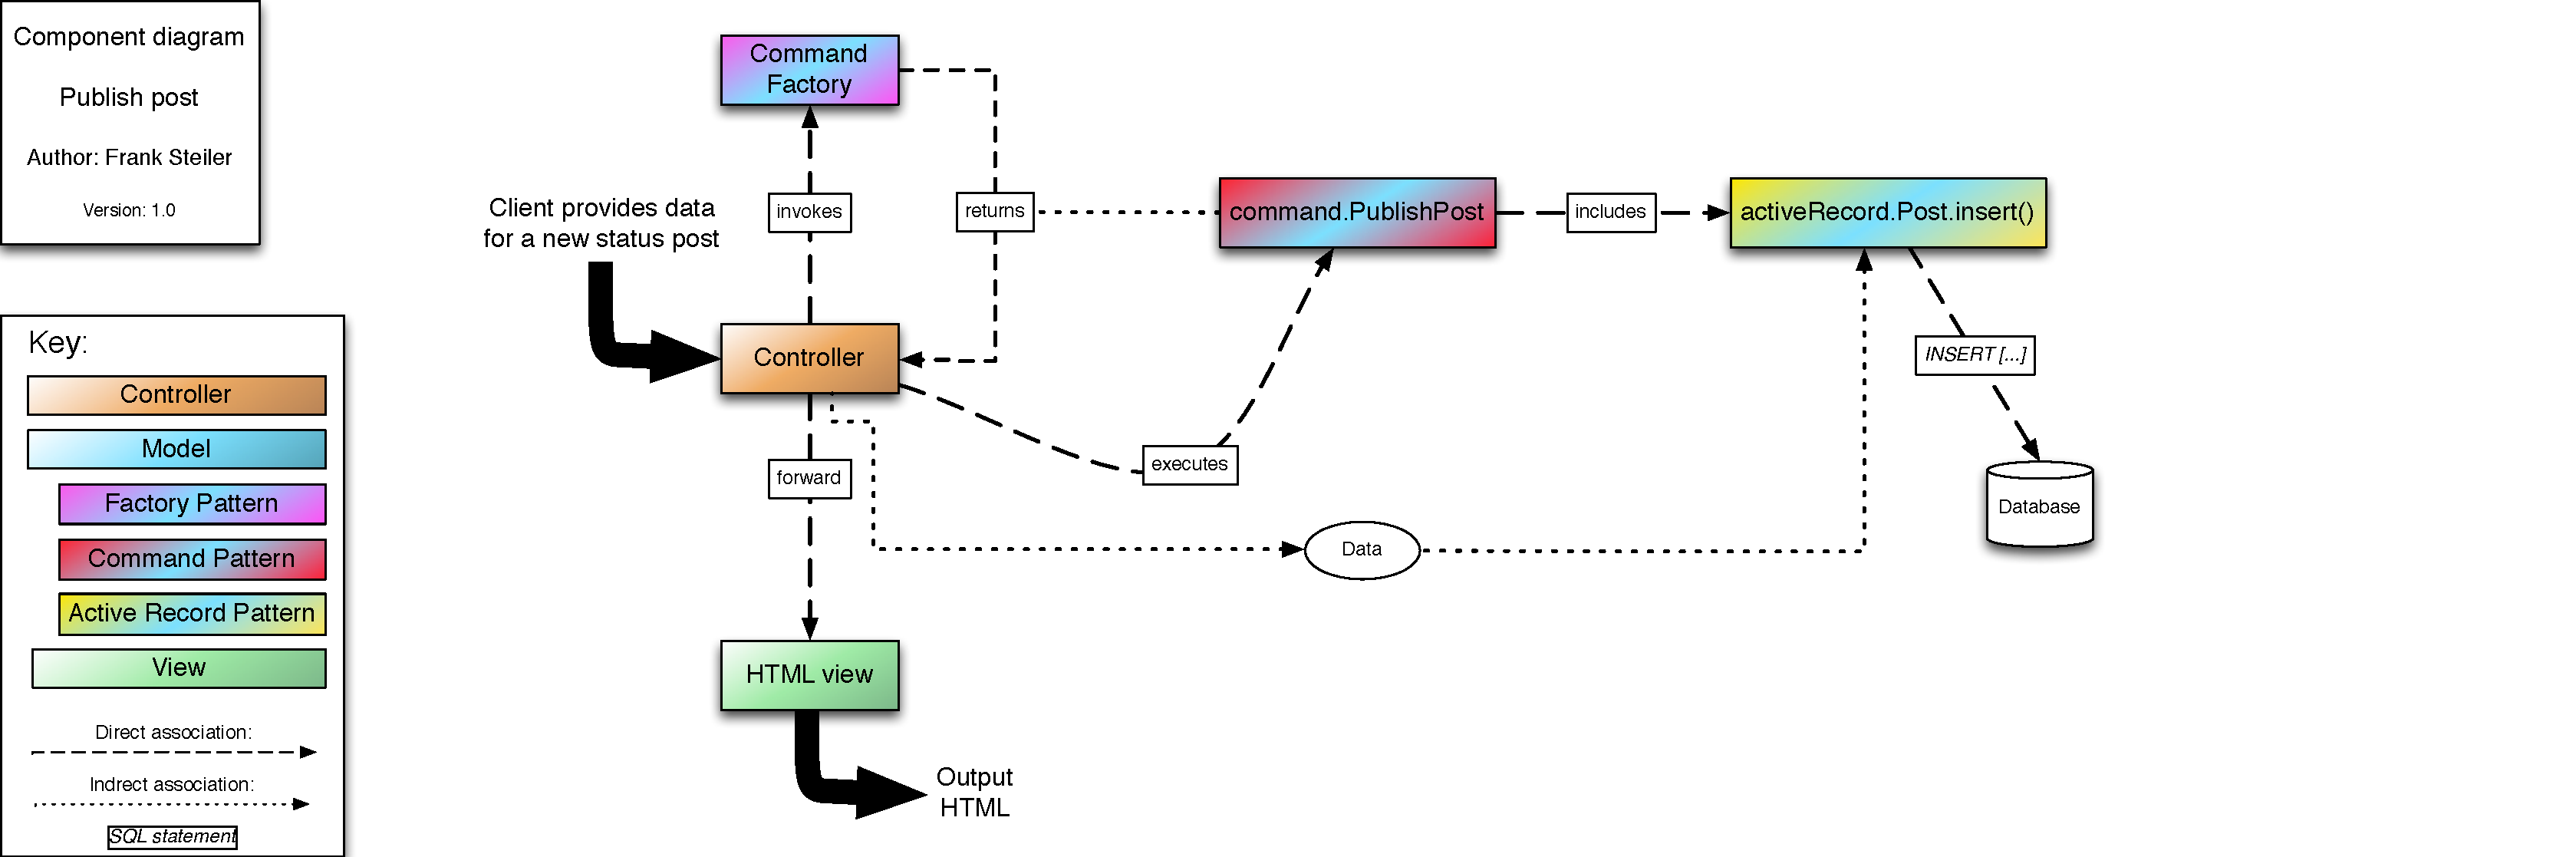
\includepdf[fitpaper=true,pages=-,addtotoc={1,section,1,Component diagram - Publish Post,app:ComponentPublishPost}]{./Appendix/Component_diagram_PublishPost.pdf}
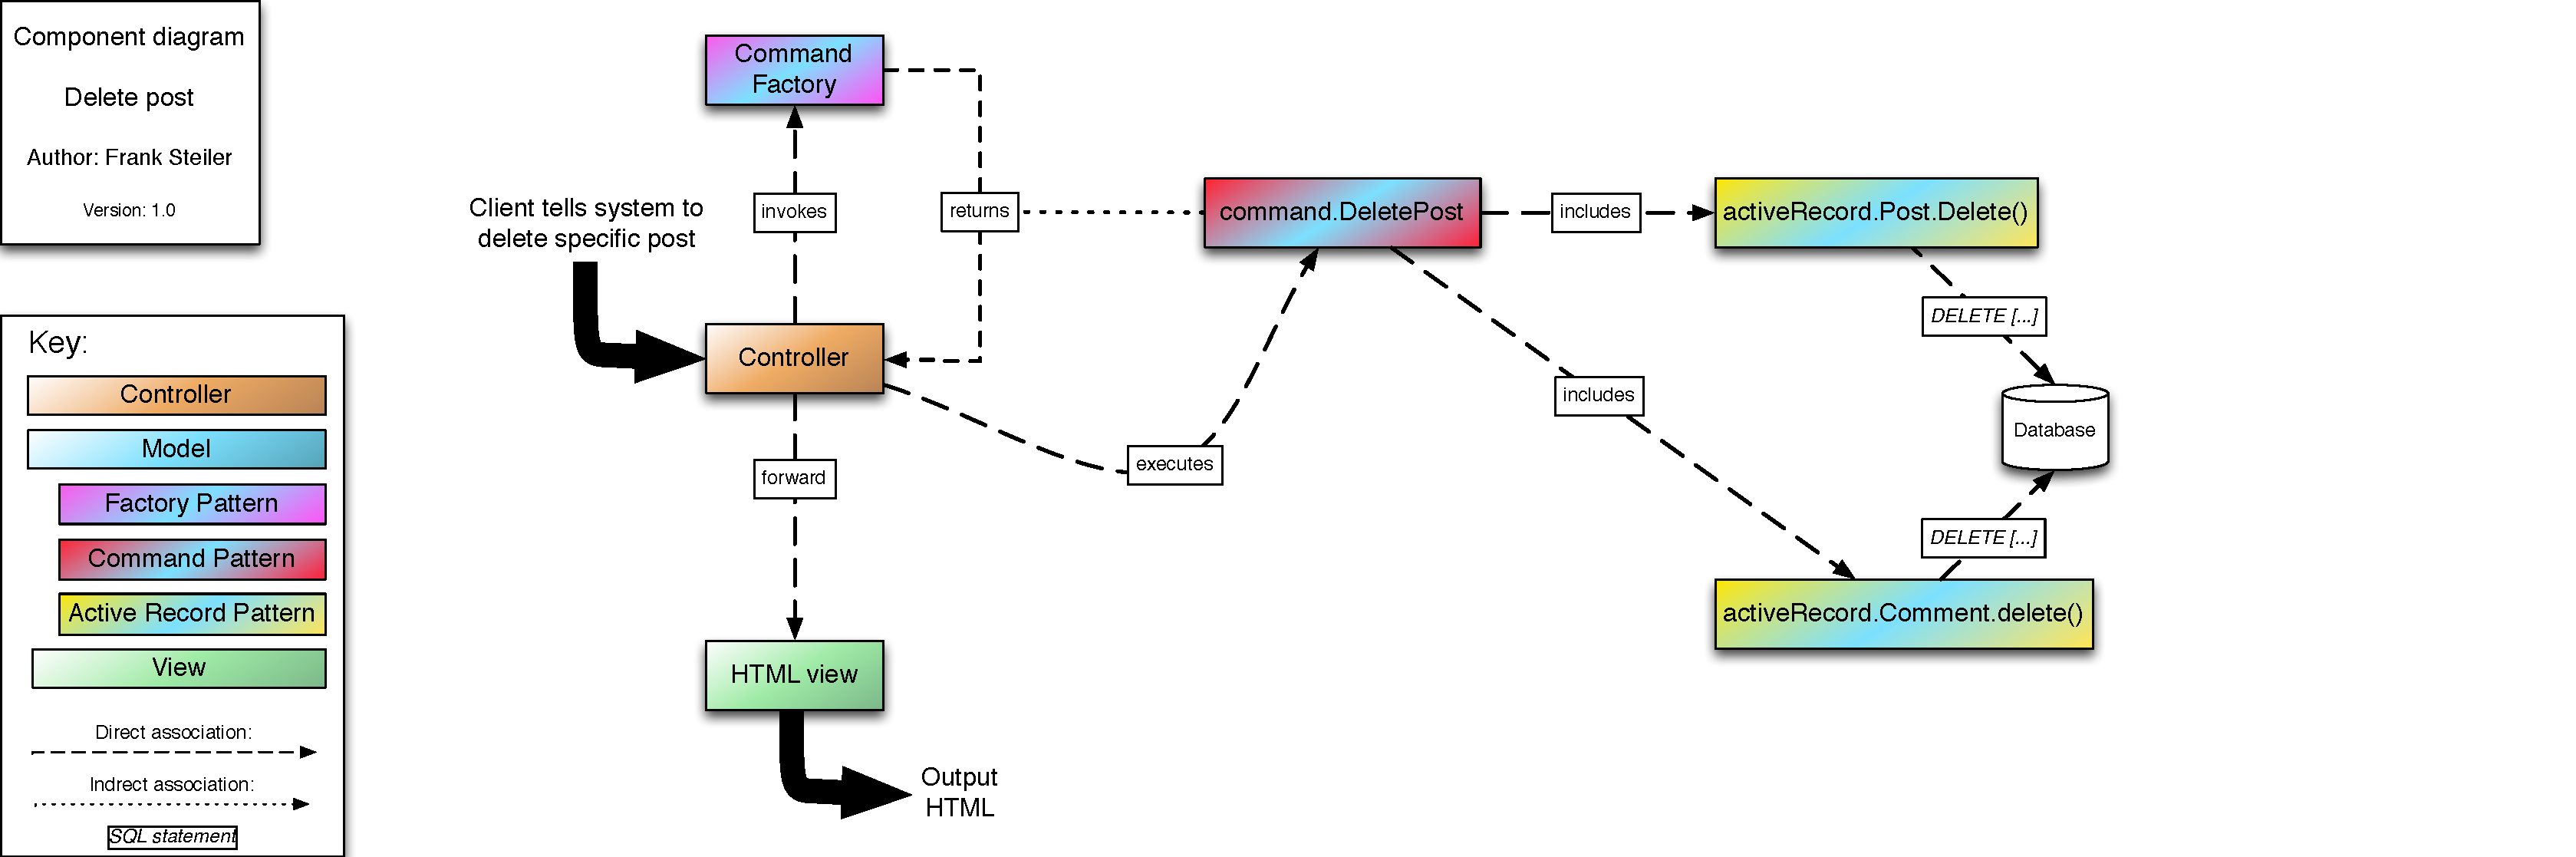
\includepdf[fitpaper=true,pages=-,addtotoc={1,section,1,Component diagram - Delete Post,app:ComponentDeletePost}]{./Appendix/Component_diagram_DeletePost.pdf}
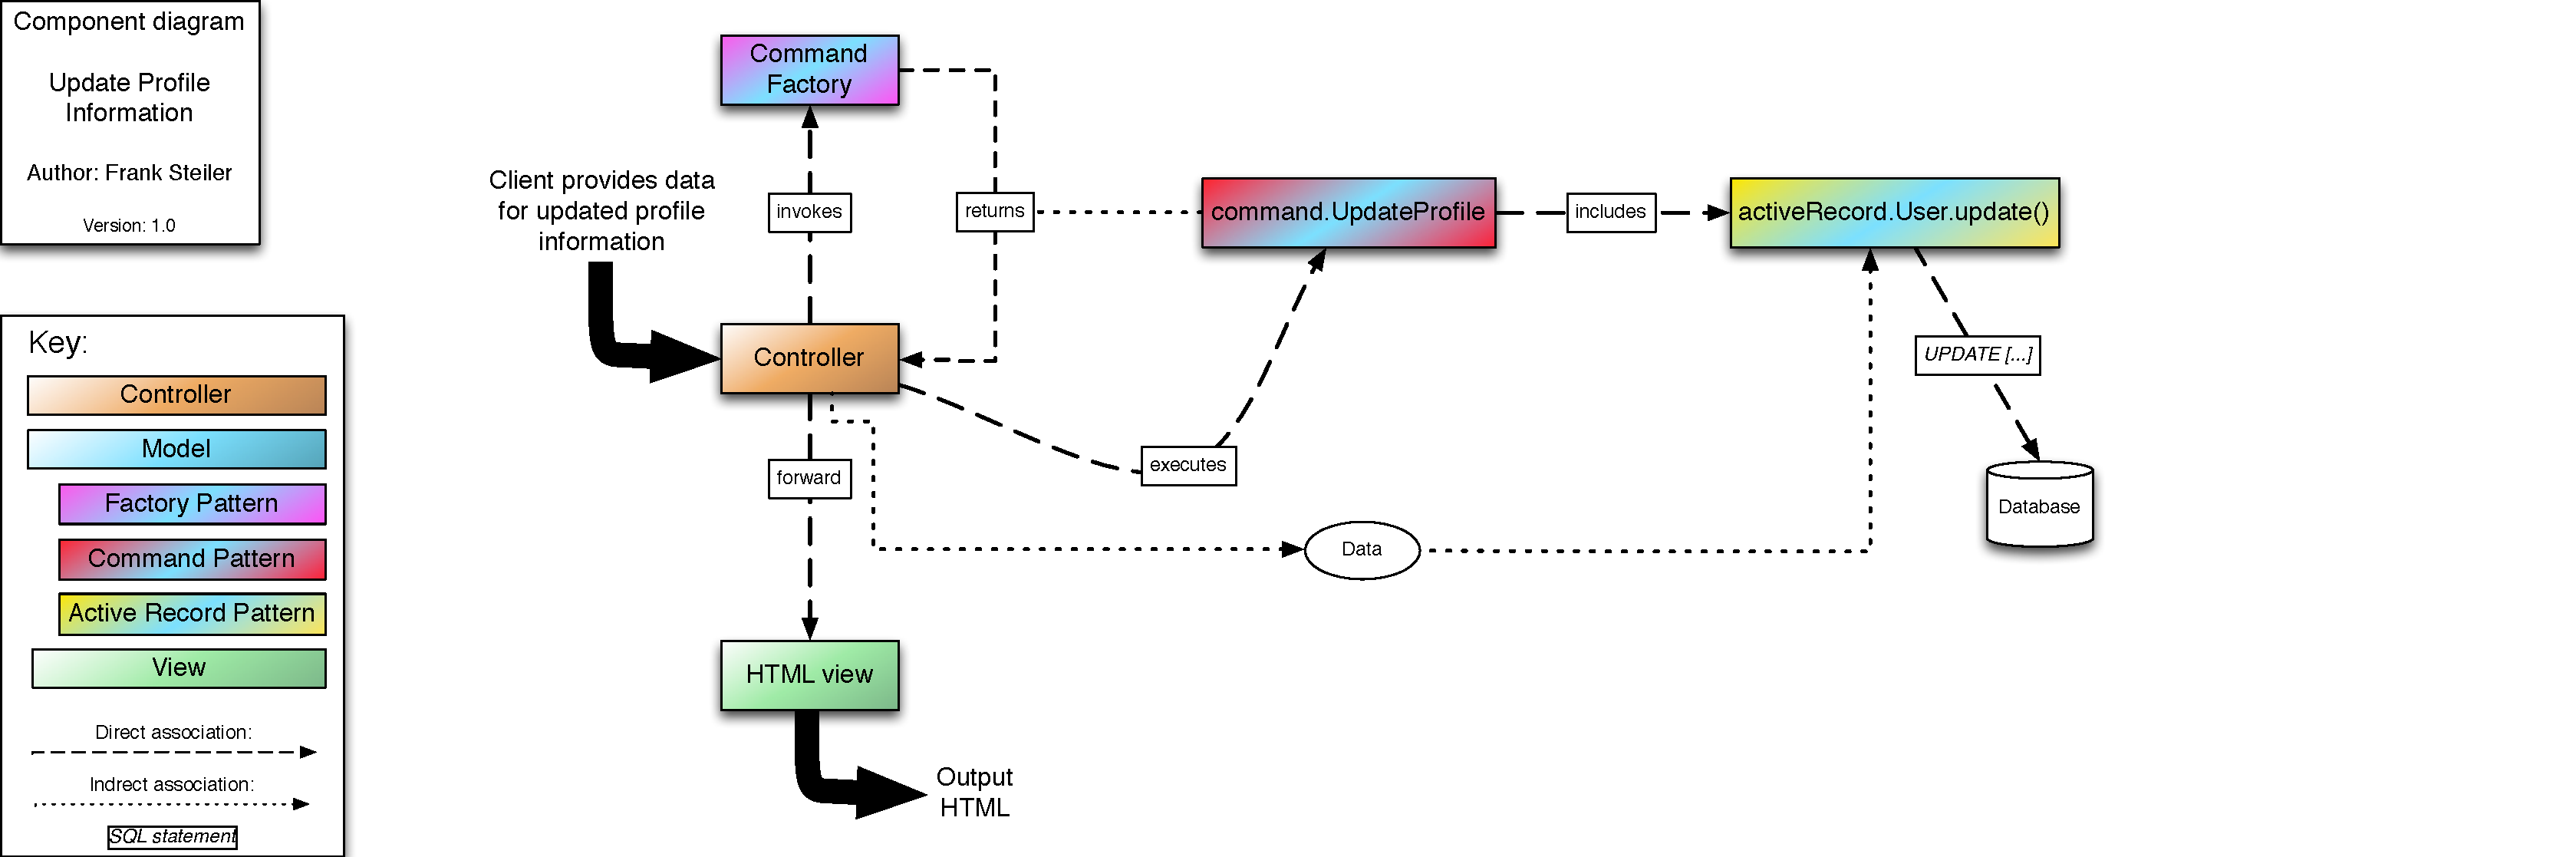
\includepdf[fitpaper=true,pages=-,addtotoc={1,section,1,Component diagram - Update Profile,app:ComponentUpdateProfile}]{./Appendix/Component_diagram_UpdateProfile.pdf}

%Risk assessment
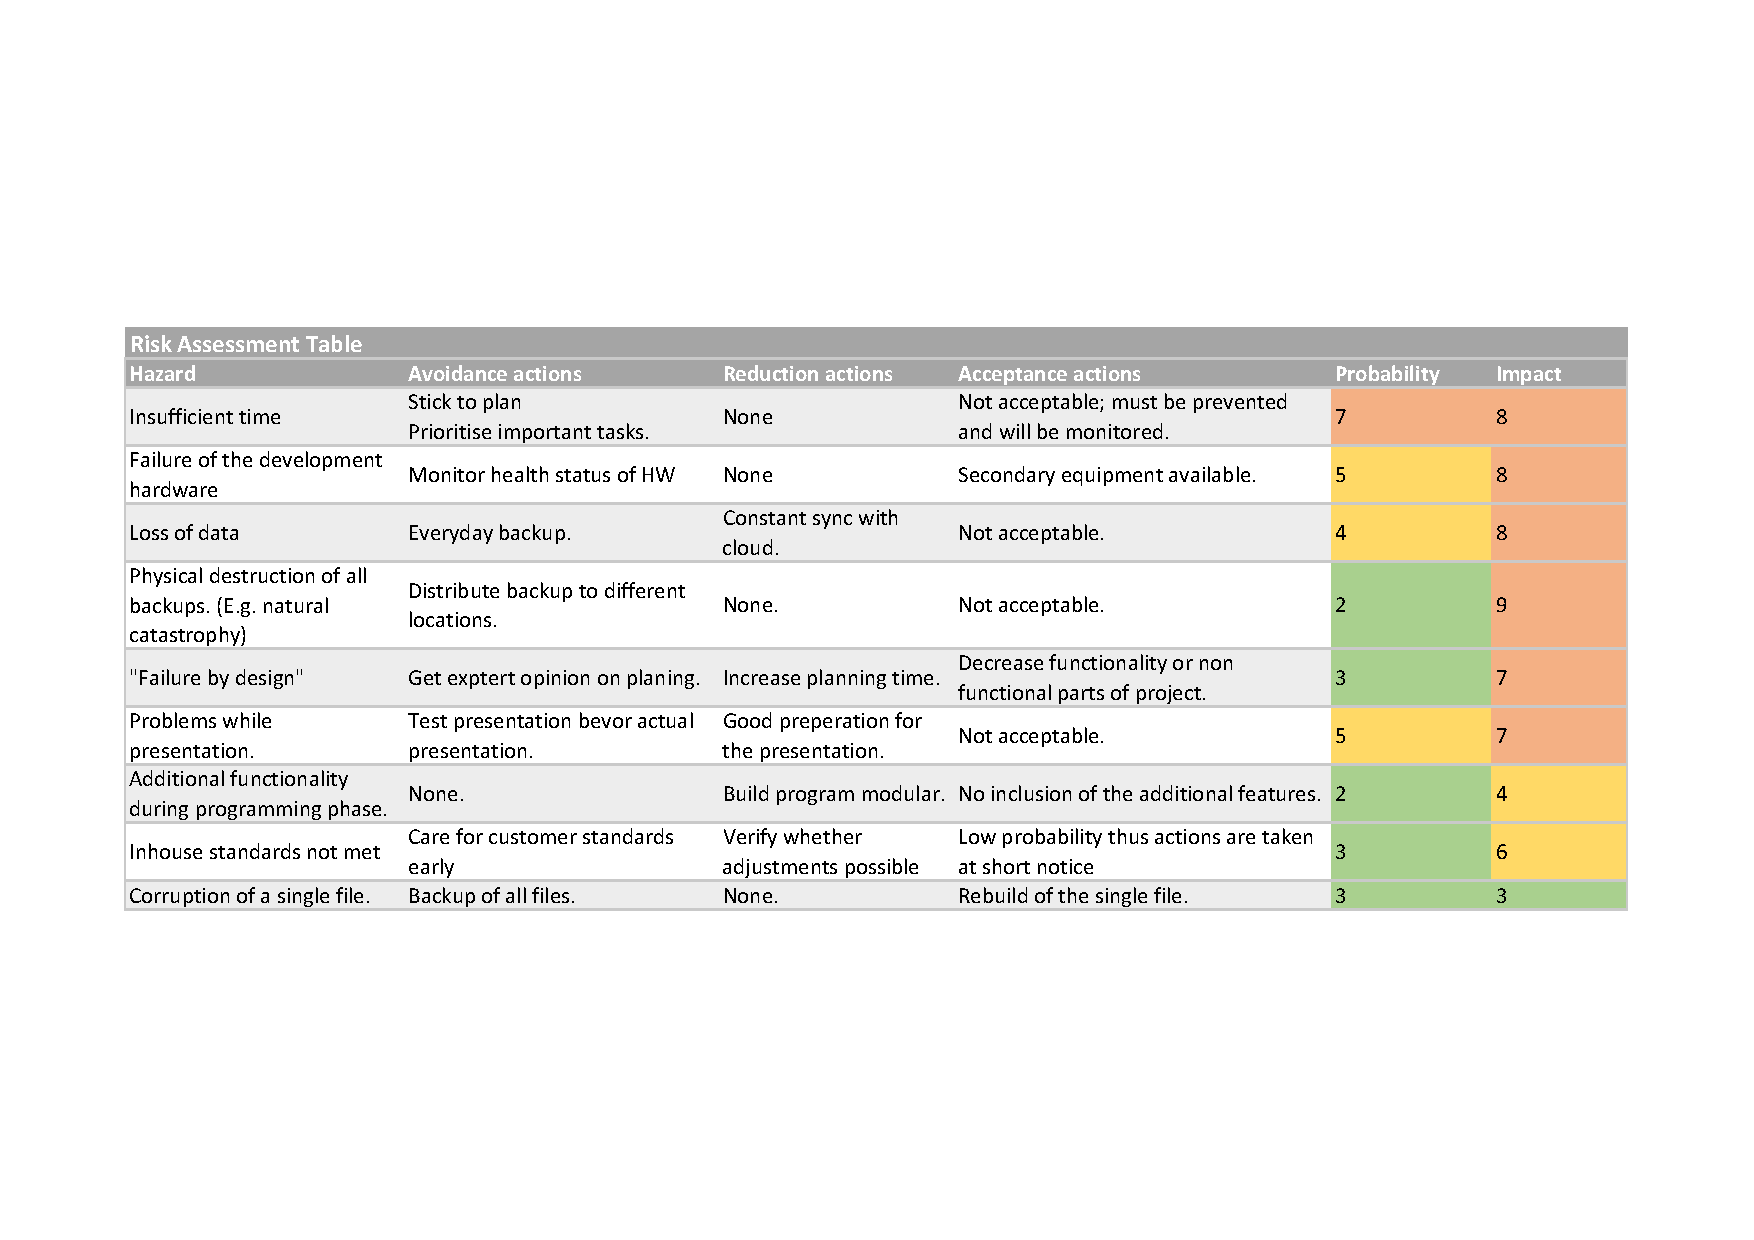
\includepdf[fitpaper=true,pages=-, addtotoc={1,chapter,0,Risk Assessment Table,app:RiskAssessmentTable}]{./Appendix/Risk_Assessment_Table.pdf}
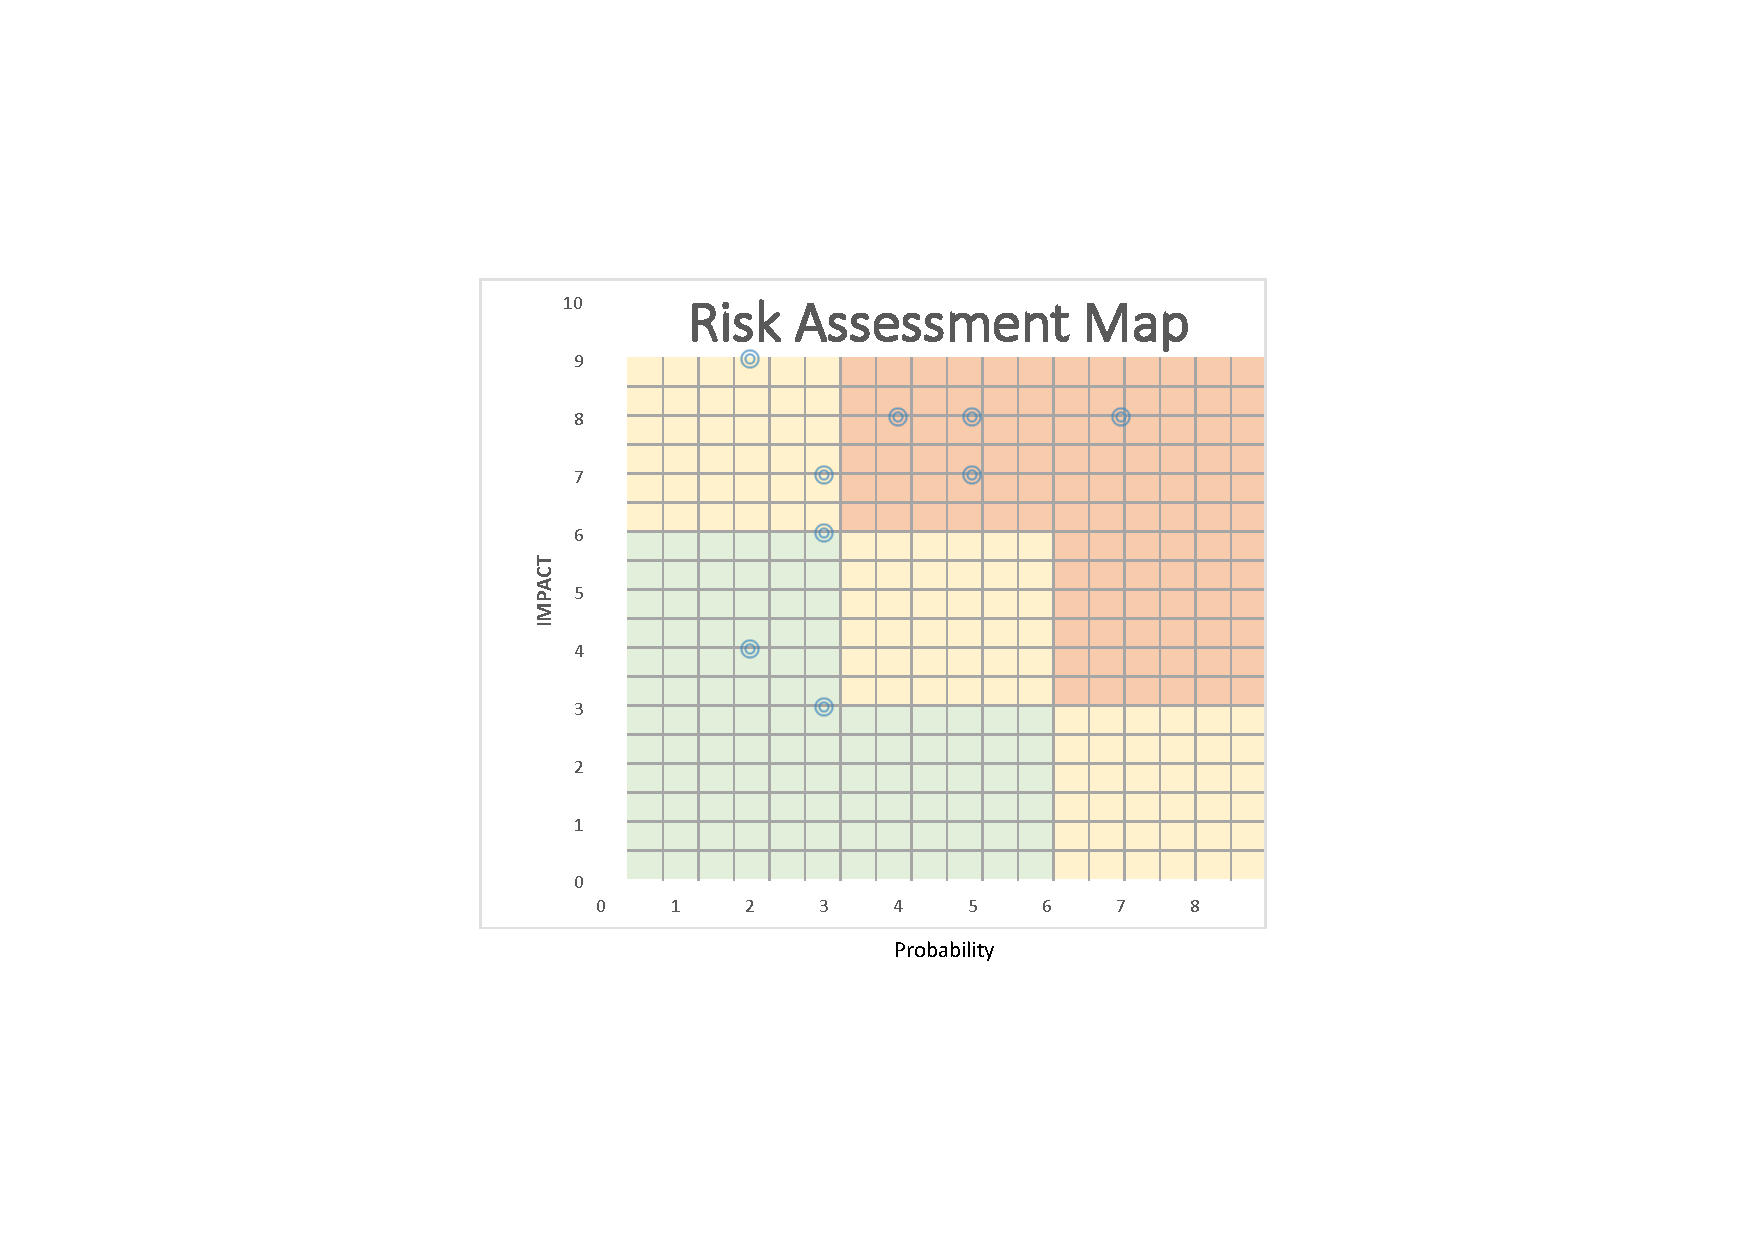
\includepdf[fitpaper=true,pages=-, addtotoc={1,chapter,0,Risk Assessment Map,app:RiskAssessmentMap}]{./Appendix/Risk_Assessment_Map.pdf}

\end{appendices}

\end{document}